\documentclass[a4paper,%
				12pt,%
				oneside%
				]{book}
				
\usepackage[english,italian]{babel}

%\usepackage[T1]{fontenc} % Riga da togliere se si compila con PDFLaTeX
\usepackage[utf8]{inputenc} % Consente l'uso caratteri accentati italiani
\usepackage{graphicx}
\usepackage{fancyhdr}
\usepackage{setspace}
\usepackage{subfig}
\usepackage{caption}
\usepackage[backend=bibtex]{biblatex}
\usepackage{amsmath}
\usepackage{amsthm}
\usepackage{moreverb}
%\usepackage[hidelinks]{hyperref}
\usepackage[bookmarks=true,pdfborder={0 0 0}]{hyperref}
\usepackage{float}
\usepackage{array}
\usepackage{tabularx}
%\usepackage{epstopdf}
\usepackage{longtable}
\usepackage[table]{xcolor}
\usepackage{color}
\usepackage{latexsym}
\usepackage{amssymb}
\usepackage{amsmath}
\usepackage{listings}
\usepackage{pgfplots}
\usepackage{algpseudocode}
\usepackage[chapter]{algorithm}




\bibliography{Bibliografia}


\graphicspath{{./Immagini_fake/}}

\nocite{*}

\setcounter{secnumdepth}{3}
\setcounter{tocdepth}{2}

\frenchspacing % forza LaTeX ad una spaziatura non inglese
\hoffset + 0.5cm

\renewcommand{\sectionmark}[1]{%
\markboth{\MakeUppercase{%
\thesection. \ #1}}{}}


\rhead{\thesection \sectionmark}
%\lhead{}
\lfoot{}%\emph{Francesco Capozzo}}
\cfoot{\thepage}
\rfoot{}
\renewcommand{\headrulewidth}{0.4pt}
\renewcommand{\footrulewidth}{0.4pt}


\renewcommand{\contentsname}{Sommario}
\renewcommand{\listfigurename}{List of Figures}
\renewcommand{\listtablename}{List of Tables}
\renewcommand{\bibname}{Bibliografia}
\renewcommand{\indexname}{Indice}
\renewcommand{\figurename}{Figura}
\renewcommand{\tablename}{Tavola}
\renewcommand{\partname}{Parte}
\renewcommand{\chaptername}{Capitolo}
\renewcommand{\appendixname}{Appendice}
\renewcommand{\today}{\ifcase\month\or
  Gennaio\or Febbraio\or Marzo\or Aprile\or Maggio\or Giugno\or
  Luglio\or Agosto\or Settembre\or Ottobre\or Novembre\or Dicembre\fi
  \space\number\day, \number\year}
  
  
%riduce lo split delle footnote
\interfootnotelinepenalty=10000


\newtheorem{thm}{Teorema}

\theoremstyle{definition}
\newtheorem{defn}{Definizione}


\floatstyle{boxed}
%\newfloat{program}{thp}{lop}[chapter]
\newfloat{program}{tbphH}{lop}[chapter]
\floatname{program}{Codice}

\newcommand{\codefrom}[2][CLIPS]
{
\begin{program}[p]
    \lstinputlisting[language=#1]{#2}
    \caption{#2}
    \label{#2}
\end{program}
}

%\newenvironment{program}{\begin{boxedverbatim}}{\end{boxedverbatim}}


% Vincoli

% Initializing the counters and define a custom label
\newcommand{\vincoliinit}{
    % Create a new counter for keeping track of the last number
    \newcounter{vincolicountbackup}
    % Create a new counter for the custom label
    \newcounter{vincolicount}
    % Redefine the command for the last counter so when it is called
    % it prints the number like this in a bold font: R<number>
    \renewcommand{\thevincolicount}{\textbf{Vincolo-\arabic{vincolicount}: }}
}

% Used to define the start of the requirements
\newcommand{\vincolistart}{
    % Indicate the start of a new list and tell it to use the redefined
    % command and corresponding counter for every item
    \begin{list}{\thevincolicount}{\usecounter{vincolicount}}
    % Important part: set the value of the used counter to the
    % same value of the backup counter.
    \setcounter{vincolicount}{\value{vincolicountbackup}}
}

% Used to define the end of the requirements
\newcommand{\vincoliend}{
    % Important part: take the value of the used counter (after
    % being incremented by the requirement items) and store it
    % in the backup counter.
    \setcounter{vincolicountbackup}{\value{vincolicount}}
    % Mark the end of the list environment
    \end{list}
}


% COLORI

\definecolor{grigio-chiarissimo}{rgb}{0.9,0.9,0.9}


% grafici

%\pgfplotsset{/pgf/number format/use comma,compat=newest}

\lstset{%
	basicstyle=\footnotesize\ttfamily,
	frame=single,
	captionpos=b,
	breaklines=true,
	tabsize=2,
	numbers=left
}

\renewcommand{\lstlistingname}{Codice}                  % file con le impostazioni personali

				
\begin{document}

\pagenumbering{roman}
\pagestyle{plain}

% !TEX root = ../Tesi.tex

\begin{center}

\includegraphics[height=2cm]{Immagini/logo.png}\\
\LARGE{UNIVERSITA' DEGLI STUDI DI BARI}\\
%\Huge{\textbf{ALDO MORO}}\\
\LARGE{ALDO MORO}\\
\vspace{0.5cm}
\small{FACOLTA' DI SCIENZE MATEMATICHE, FISICHE E NATURALI}\\
CORSO DI LAUREA IN\\
INFORMATICA\\
\hrulefill \\ %liena oritizontale
\vspace{0.2cm}
TESI DI LAUREA\\
\vspace{0.2cm}
IN\\
\vspace{0.2cm}
\normalsize{INGEGNERIA DELLA CONOSCENZA E SISTEMI ESPERTI}\\
\vspace{2cm}%inserisci una riga vuota(spazio rigido 
\large{\textbf{.\ .\ .\ }}\\
\thispagestyle{empty}%per non numerare la prima pagina
\end{center}
\vspace{3cm}
RELATORI:\\
Chiar.ma Prof.ssa Floriana Esposito\\
Chiar.mo Prof Stefano Ferilli

\begin{flushright}
LAUREANDO:\\
Francesco Capozzo\\
\end{flushright}
\hrulefill
\begin{center}
\small{ANNO ACCADEMICO 2011/2012}
\end{center}

\pagestyle{fancy}

%\doublespacing
\onehalfspacing

 

\singlespacing
\rhead{}

\tableofcontents % Prepara l'indice generale
\listoffigures
\listoftables

\doublespacing

 

\chapter*{Prefazione}
\addcontentsline{toc}{chapter}{Prefazione}
\chaptermark{Prefazione}
\rhead{}

Gli strumenti di sviluppo per sistemi esperti hanno vissuto un periodo di grande fermento durante gli anni '80. L'introduzione di nuove tecniche algoritmiche, che permettessero la distribuzione e l'utilizzo dei sistemi prodotti su hardware di comune reperibilità, ha traghettato i sistemi basati su conoscenza da strumenti orientati alla ricerca anche verso ambiti con implicazioni più pratiche. Il grande passo avanti compiuto con la creazione di \emph{environment} in linguaggi diffusi ed efficienti come il C ha offerto la possibilità di adottare queste tecnologie anche in situazioni dove le risorse disponibili, sia economiche che computazionali, risultavano relativamente limitate. Il nuovo \emph{boom} tecnologico catalizzato dall'avvento di \emph{Internet} sta portando ad un cambiamento radicare nel modo di concepire il software ed i meccanismi di distribuzione. Il fenomeno sta portando alla luce molti dei limiti dei prodotti concepiti e realizzati prima dell'avvento del \emph{web}. Valori come le prestazioni e l'efficienza nella gestione delle risorse, pur rimanendo fattori importanti, sono sempre più spesso messi in secondo piano davanti a criteri di scelta legati alla rapidità e la facilità di sviluppo. La proprietà di un sistema di poter essere adattato più facilmente e più velocemente al repentino cambiamento delle necessità  è diventato un elemento chiave in qualsiasi scelta di sviluppo software.

Lo scopo di questo lavoro di tesi, realizzato presso il laboratorio LACAM del dipartimento di Informatica dell'Università degli Studi di Bari, è quello proporre un \emph{expert system environment} che renda agevole l'attività di integrazione dei sistemi esperti anche nei contesti che richiedano l'utilizzo di tecnologie per la distribuzione dei servizi tramite il web.

Nel primo capitolo si fornirà una panoramica sui sistemi esperti, il loro ambito di utilizzo e il processo di sviluppo. Si descriveranno le modalità di rappresentazione della conoscenza e si introdurranno le principali tecniche coinvolte per la realizzazione dell'inferenza e del ragionamento basato su regole, focalizzandosi sulla descrizione del problema del confronto fra stato del sistema e base di conoscenza. Verrà quindi effettuata una panoramica sugli strumenti di supporto allo sviluppo dei sistemi esperti fornendone una classificazione in base alle funzionalità e caratteristiche.

Nel secondo capitolo si approfondiranno le problematiche relative alla realizzazione di un \emph{environment} per sistemi esperti, analizzandone le componenti chiave e fornendo una descrizione delle tecniche utilizzate e delle capacità richieste per il prototipo realizzato in questo lavoro di tesi.

Nel terzo capitolo  si affronteranno le tematiche relative alla progettazione ed all'implementazione del sistema, secondo i vincoli evidenziati nel secondo capitolo. Verrà fornita una descrizione sommaria delle delle componenti che realizzano il sistema e degli algoritmi utilizzati dallo stesso. Si passerà quindi ad una sperimentazione del prototipo, necessaria per valutarne la correttezza e le prestazioni, offrendo un confronto con una soluzione di riferimento nel campo degli \emph{environment} come lo è CLIPS.

\rhead{\thesection \sectionmark}

\mainmatter
\chapter{Environment per Sistemi Esperti}

\setcounter{section}{1}
\phantomsection\addcontentsline{toc}{section}{\protect\numberline{\thesection}Sistemi Esperti}
\sectionmark{Sistemi Esperti}

\begin{quote}
''Un esperto è una persona alla quale, per motivi professionali o per una acquisita competenza ed esperienza su una data materia, viene richiesto di fornire pareri scientifici su argomenti di dettaglio.'' (Wikipedia)
\end{quote}

Sembra ragionevole la scelta di attribuire l'aggettivo di \emph{esperto} a una persona in possesso di qualità e caratteristiche che ne attestino una conoscenza in uno specifico ambito di dominio e che sia in grado di risolvere direttamente problemi o fornire possibili soluzioni in seguito ad una attività di ragionamento.
Realizzando un parallelismo, è possibile considerare l'assegnazione dell'attributo di \emph{esperto} ad un sistema in grado di esibire un comportamento paragonabile a quello di un esperto umano all'interno di un ambito di dominio focalizzato.
La definizione fornita in \cite{jackson1999} spiega il \emph{sistema esperto} come un'applicazione che rappresenta e ragiona con conoscenza di tipo specialistico con l'obiettivo di risolvere problematiche o fornire consigli su come risolverle.

L'obiettivo di utilizzo di un \emph{sistema esperto} può essere quello di sostituire completamente l'intervento umano durante lo svolgimento di un'attività o di fornire supporto ad un esperto durante l'atto di prendere una decisione, giocando un ruolo di assistenza. Altre possibili applicazioni possono riguardare la formazione o il perfezionamento della conoscenza posseduta da un esperto tramite l'interazione diretta con il sistema a titolo di confronto o consultazione.

I sistemi esperti sono applicazioni progettate per rendere disponibili alcune abilità di esperti di un dominio anche a utenti non esperti. Siccome questo genere di programmi tentano di emulare gli schemi mentali e i modi di pensare di un esperto, è naturale che le prime ricerche in questo ambito siano state effettuate nel campo dell'\emph{intelligenza artificiale}: una branca delle Scienze Informatiche correlate con la progettazione e la realizzazione di applicazioni in grado di emulare le abilità cognitive umane nel campo della soluzione di problemi, la percezione e la comprensione del linguaggio~\cite{feigenbaum1981ia}.

Ciò che differenzia un'applicazione convenzionale da un \emph{sistema esperto} può essere sintetizzato in tre caratteristiche fondamentali: perché ragiona; su cosa ragiona; come ragiona.

L'obiettivo di un sistema esperto è quello di simulare un ragionamento umano nell'ambito di un dominio, piuttosto che simulare il dominio stesso. Le applicazioni convenzionali lavorano attraverso la realizzazione di un modello matematico al fine simulare le abilità dell'esperto nella soluzione del problema. I sistemi esperti invece focalizzano l'attenzione sull'emulazione degli schemi di ragionamento che l'esperto adotta per ottenere delle soluzioni e tentano di emulare il processo di ragionamento e non semplicemente il risultato allo specifico problema.

Un altro fattore discriminante riguarda il tipo di informazioni sulle quali i due sistemi lavorano: le applicazioni tradizionali utilizzano modelli per rappresentare il problema, applicano algoritmi per la manipolazione dei dati ed infine calcolano soluzioni. Nei sistemi esperti, invece, l'intero processo di ragionamento viene eseguito lavorando su rappresentazioni della conoscenza umana. Queste rappresentazioni vengono codificate utilizzando linguaggi specificamente sviluppati e che permettono di separare la rappresentazione della conoscenza di dominio dalle porzioni del sistema che invece rappresentano le dinamiche di ragionamento. Queste due porzioni dei sistemi esperti vengono definite con i nomi di \emph{base di conoscenza} e \emph{motore inferenziale}.

Le meccaniche di soluzione rappresentano l'ultimo fattore di differenza: se le applicazioni tradizionali risolvono problematiche offrendo soluzioni algoritmiche a problemi per i quali è stato individuato un modello, i sistemi esperti ottengono soluzioni applicando metodi approssimati o \emph{euristiche}\footnote{L’\emph{euristica} è una strategia cognitiva, una scorciatoia di pensiero, una tecnica basata su esperienze, che permette più rapidamente di elaborare giudizi, ricavare inferenze dal contesto, attribuire significato alle situazioni e prendere decisioni a fronte di problemi complessi o di informazioni incomplete~\cite{euristiche1}~\cite{kahneman1982judgment}.} spesso utilizzando conoscenza incerta o incompleta.

Proprio a causa della natura dinamica e incerta del ragionamento alla base dei \emph{sistemi esperti}, a questa classe di sistemi viene richiesta la capacità di interagire con l'utente (sia esso un esperto o no) in modo da:
\begin{itemize}
	\item illustrare e spiegare il ragionamento adottato per ottenere delle soluzioni e giustificare in questo modo il suo operato; 
	\item interagire con il mondo esterno tramite specifici protocolli, in modo da rendere possibile il reperimento di informazioni aggiuntive, qualora queste risultassero necessarie, durante il processo di ragionamento.
\end{itemize}

\begin{quotation}
''La \emph{vera} intelligenza richiede l'abilità di imparare, di ragionare sull'esperienza, d'agire d'istinto\footnote{L'espressione originale usava la forma gergale \emph{''to shoot from the hip''} la cui traduzione letterale rimanda al movimento dei cowboy di sparare velocemente dal fianco senza mirare con precisione.}, di usare conoscenza generale, di fare inferenza usando intuizioni \emph{viscerali}. I sistemi esperti non fanno niente di tutto ciò, Non migliorano i risultati sulla base dell'esperienza. Loro [i sistemi esperti] sanno soltanto spostarsi da una regola \emph{if/then} all'altra.'' \cite{schank1984ia} 
\end{quotation}

La capacità di apprendimento, che per Schank \cite{schank1984ia} è uno dei fattori determinanti per poter associare al ragionamento dei sistemi esperti l'attributo di \emph{intelligente}, rappresenta un'ulteriore componente chiave nella definizione di sistemi esperti. Alcune tecniche basate sull'aggiunta di nuovi elementi nella base di conoscenza o sull'aggiunta di nuove euristiche hanno permesso di integrare meccanismi di apprendimento automatico all'interno dei sistemi esperti~\cite{nasa1988flops}.

Dalla metà degli anni '60 ad oggi  sono stati creati un gran numero di sistemi esperti con ambiti di utilizzo molto differenti fra loro. Per fare alcuni esempi è possibile citare quello aerospaziale (ad esempio per agevolare alcune operazioni in orbita), quello sanitario (ad esempio nell'assistenza al monitoraggio dei parametri dei pazienti nelle unità di terapia intensiva o nella diagnosi di malattie) o quello finanziario.~\cite{jackson1999}

Il primi sistemi esperti prodotti furono Dendral (1965), con lo scopo di determinare la struttura molecolare partendo da dati provenienti da uno spettrometro di massa, R1 (1978), usato per configurare sistemi informatici e MYCIN (1976), per assistere nella diagnosi di infezioni da batteri e proporre piani terapeutici per il trattamento delle stesse.

\subsection{Le componenti di un sistema esperto} 

\begin{figure}[h]
\centering
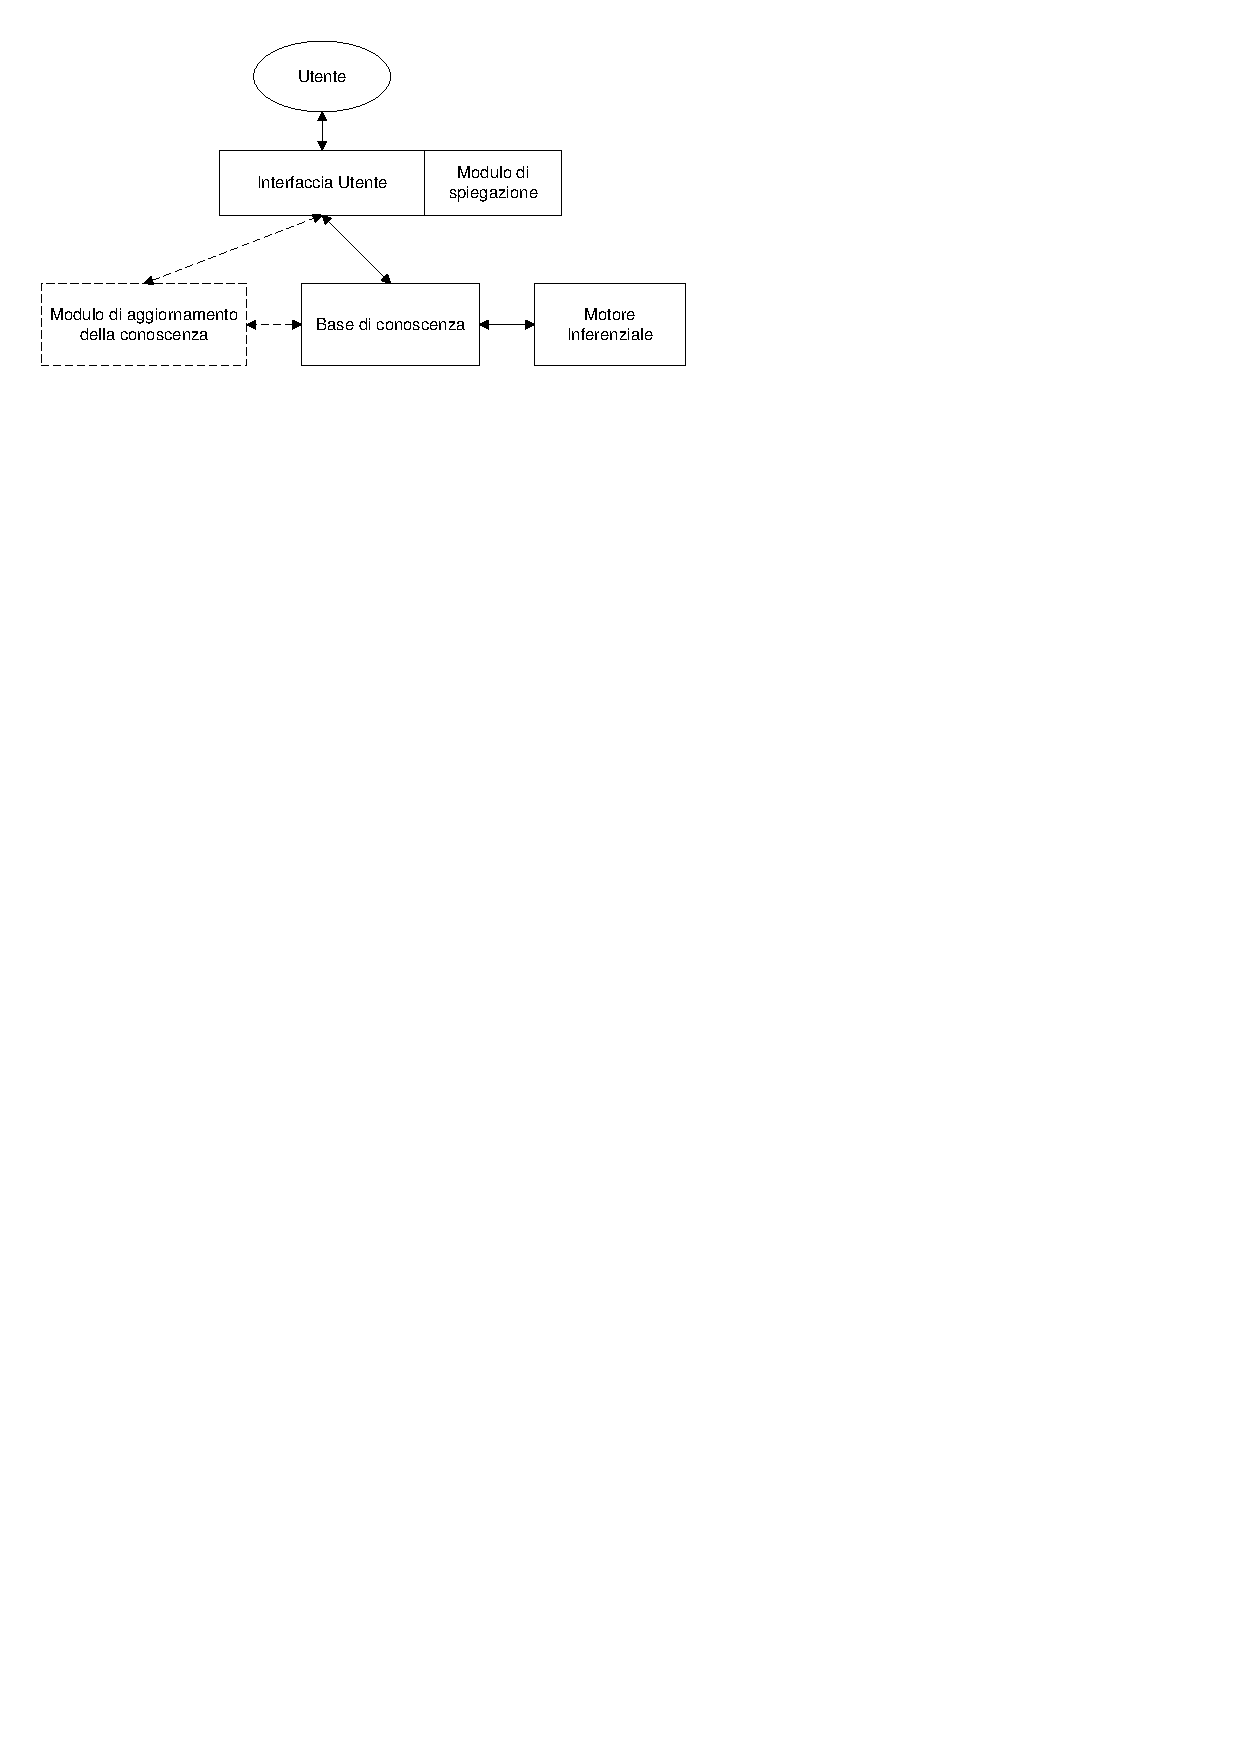
\includegraphics[viewport=19 667 329 824]{Immagini/Capitolo1/Architettura-SE.pdf}
\caption{Architettura semplificata di un generico Sistema Esperto}\label{fig:architettura-se}
\end{figure}

La struttura di un sistema esperto può essere sinteticamente descritta come composta da quattro moduli principali~(\figurename~\ref{fig:architettura-se}):
\begin{itemize}
	\item \emph{La base di conoscenza}: raccoglie tutta la conoscenza di dominio acquisita. La fonte principale d'informazione è rappresentata dall'esperto che, interrogato da un ingegnere della conoscenza, fornisce in maniera più o meno completa la conoscenza di cui dispone.
	\item \emph{Il motore inferenziale}: raccoglie i processi di ragionamento sulla base dei quali il sistema, usando congiuntamente la base di conoscenza e ulteriori (ed eventuali) informazioni ottenute dall'interazione diretta con l'utente, è in grado di dedurre nuove conoscenza.
	\item \emph{L'interfaccia utente}: permette l'interazione fra l'utente e il sistema. L'interazione può essere orientata verso la spiegazione del processo logico alla base di una soluzione o una scelta (attività svolta dal \emph{modulo di spiegazione}), oppure per ottenere ulteriori informazioni e far proseguire il ragionamento.
	\item \emph{Modulo di aggiornamento della conoscenza}: permette di modificare ed integrare quanto presente nella \emph{base di conoscenza} tramite processi automatici o che richiedono l'intervento di un esperto.
\end{itemize}

\subsection{Il processo di sviluppo di un sistema esperto}
Come il processo di sviluppo di software tradizionale può essere scandito in fasi e rappresentato all'interno dei vari modelli di sviluppo, anche la produzione di sistemi esperti può essere semplificata attraverso un modello suddiviso in step successivi. 

\begin{figure}[h]
\centering
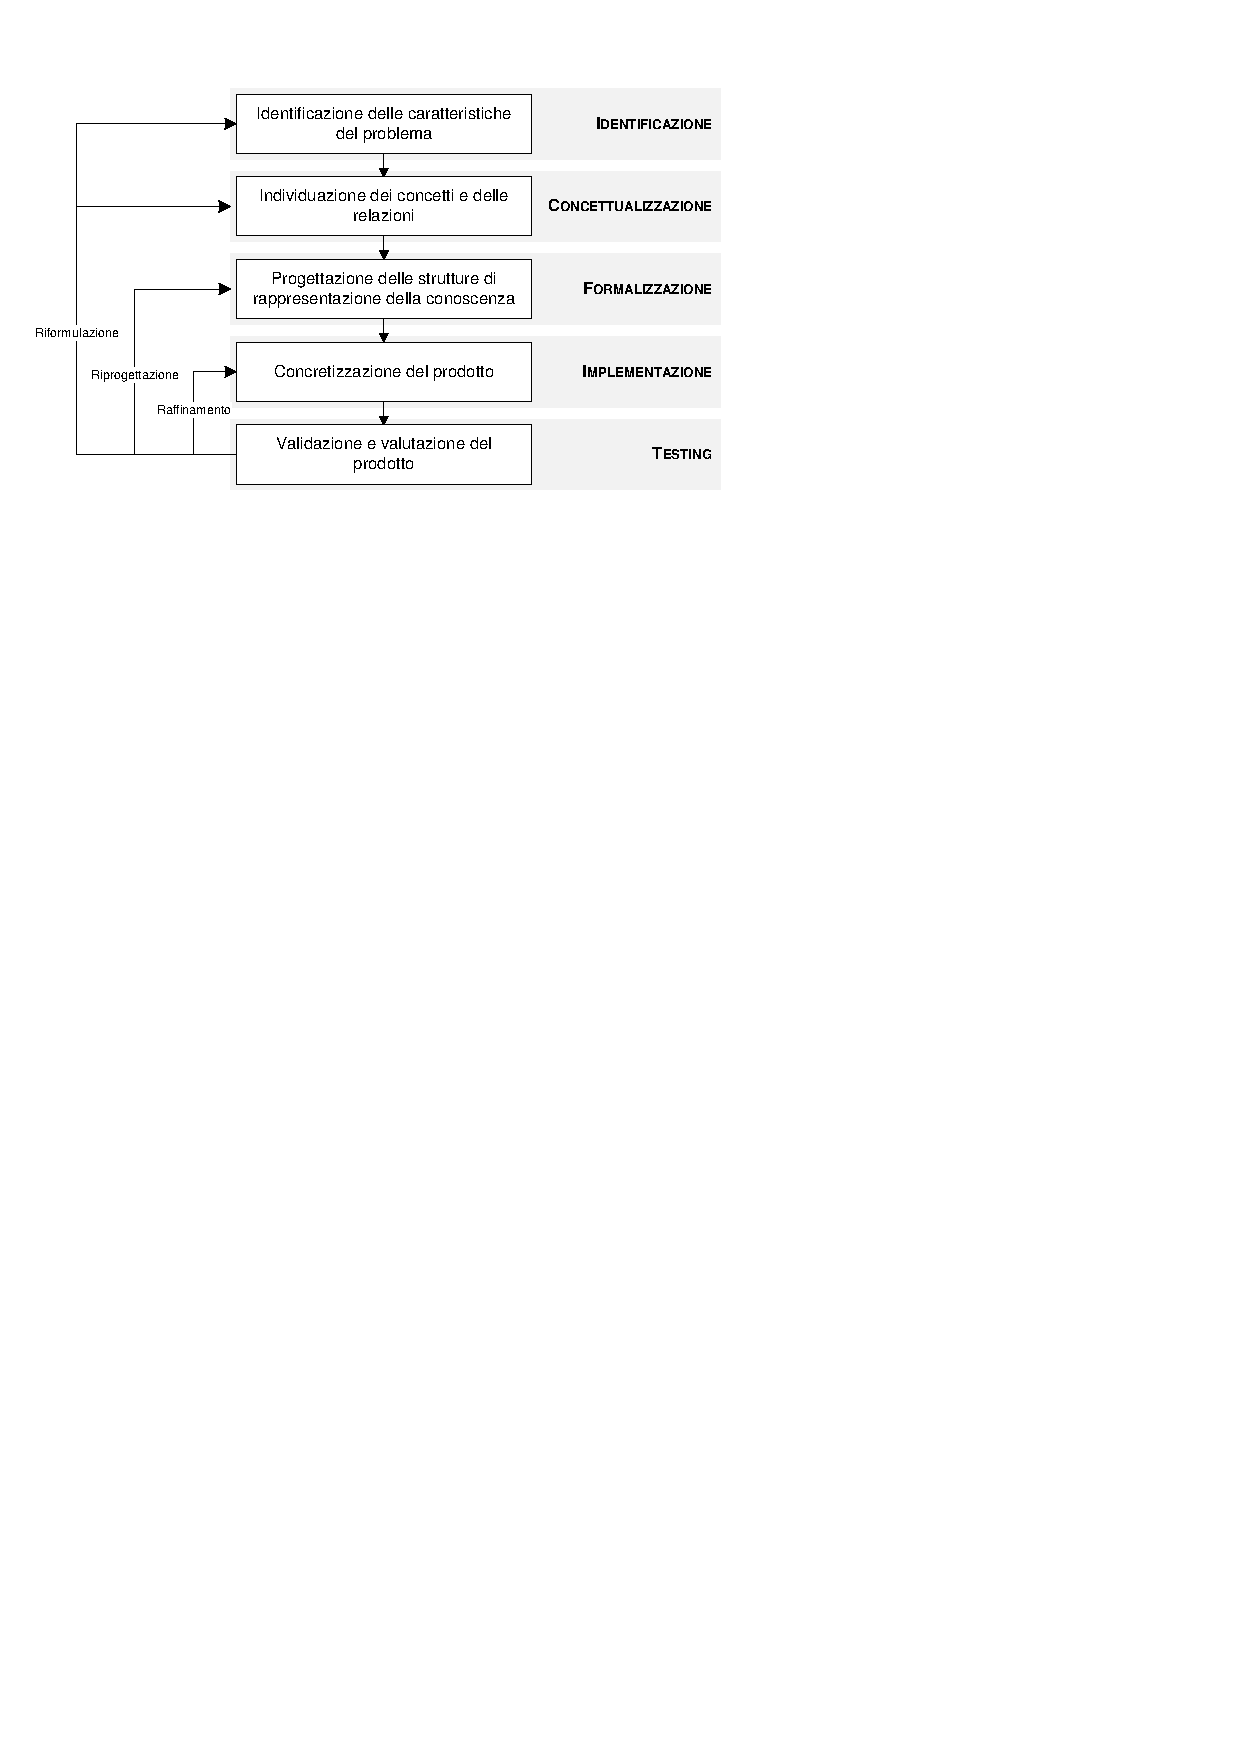
\includegraphics[viewport=16 607 346 801]{Immagini/Capitolo1/Fasi-acquisizione.pdf}
\caption{Le fasi di estrazione della conoscenza e sviluppo di un \emph{Sistema Esperto}}\label{fig:fasi-progettazione}
\end{figure}


Sebbene il confronto fra lo sviluppo di software tradizionale e quello di sistemi basati su conoscenza possa mostrare punti di contatto, le somiglianze sono solamente superficiali ed un'analisi approfondita rivelerebbe profonde differenze dettate dalle specifiche caratteristiche del tipo di artefatto in produzione.~\cite{esposito2012icse}

Alla figura già descritta dell'esperto di dominio viene affiancata quella dell'\emph{ingegnere della conoscenza}: un esperto informatico addetto alla compilazione di una base di conoscenza.

Come mostrato in \figurename~\ref{fig:fasi-progettazione} e suggerito in \cite{buchanan1983}, il processo può essere diviso in cinque fasi:
\begin{itemize}
	\item \emph{Identificazione}: è orientata all'identificazione della classe di problemi che il sistema dovrà risolvere, dei dati con i quali il sistema dovrà lavorare e dei criteri che le soluzioni dovranno soddisfare.
	
	\item \emph{Concettualizzazione}: ha la finalità di scoprire i concetti chiave e le relazioni che intercorrono fra loro. Questa fase dovrebbe includere la caratterizzazione delle varie tipologie di dati, il flusso delle informazioni e la delineazione delle strutture del dominio del problema.
	
	\item \emph{Formalizzazione}: le conoscenze e le relazioni fra le entità individuate ed organizzate nelle fasi precedenti vengono concretizzate tramite l'uso di un formalismo concordato dai membri appartenenti al team di sviluppo del sistema. In questa fase vengono eseguite le scelte relative alla tipologia di rappresentazione della conoscenza da adottare e gli strumenti da adoperare.
	\item \emph{Implementazione}: gli elementi ottenuti nei passi precedenti vengono convertiti in un artefatto completo.
	\item \emph{Testing}: l'artefatto viene sottoposto alla valutazione dell'esperto di dominio. Ne vengono valutate l'utilità e le prestazioni e verificata la corrispondenza con i requisiti fissati nelle fasi precedenti. In questa fase viene infine valutata la possibilità apportare modifiche, correggere difetti o integrare nuovi elementi nella strategia di controllo o nella base di conoscenza.
\end{itemize}

Il processo di acquisizione della conoscenza e sviluppo del sistema, sebbene possa sembrare rigoroso, non è affatto un processo lineare. Ad ogni fase viene associata un'attività di verifica e raffinamento eseguita tramite la consultazione dell'esperto di dominio.

L'attività di estrazione della conoscenza eseguita nelle fasi iniziali dello sviluppo non è un processo accurato o esente da errori: durante le interviste condotte dagli ingegneri della conoscenza, spesso, elementi importanti nell'ambito del dominio del problema vengono trasferiti dall'esperto in maniera imprecisa, errata o non esplicitati affatto (più o meno consapevolmente)~\cite{jackson1999}~\cite{schank1984ia}~\cite{buchanan1983}.

Inoltre, la natura stessa del sistema (un prodotto nel quale il ragionamento, chiave del funzionamento, viene portato avanti tramite euristiche e l'approssimazione dei modelli di ragionamento umani) lo rende un artefatto perennemente incompiuto: sarà sempre possibile integrare nuova conoscenza proveniente dall'esperto nella forma di nuovi concetti, relazioni o nuove dinamiche di controllo, modificare componenti del sistema per incrementare le prestazioni o incrementare l'affidabilità del sistema, aggiungendo nuove euristiche in grado di comprendere situazioni particolari che generavano risultati errati in versioni precedenti.

\subsection{Rappresentazione della conoscenza}

La conoscenza umana può essere raggruppata genericamente in \emph{conoscenza dichiarativa}, una forma di conoscenza esplicita rappresentante fatti, eventi ed esperienze consolidate nella forma di elementi memorizzabili, e \emph{conoscenza procedurale}. La seconda rappresenta l'insieme di abilità e conoscenze nell'utilizzo della \emph{conoscenza dichiarativa} per lo svolgimento di una attività di qualche genere.


Nell'ambito dell'ingegneria della conoscenza e dei sistemi esperti, con l'espressione \emph{Rappresentazione della conoscenza} si è soliti riferirsi alle modalità con le quali grandi quantità di informazioni utili possono essere descritte \emph{formalmente} con la finalità di essere sottoposte ad un qualche genere di \emph{manipolazione simbolica}~\cite{jackson1999}.

La \emph{descrizione formale} impone l'uso di un linguaggio o una notazione non ambigua dotata di:
\begin{itemize}
	\item una \emph{sintassi} ben definita che governa le forme di espressione;
	\item una \emph{semantica} ben definita che riveli il significato delle espressioni in virtù della forma sintattica con la quale sono codificate.
\end{itemize}

Il processo di elaborazione di simboli e strutture simboliche rappresentanti concetti e relazioni fra gli stessi è definito \emph{computazione simbolica}.

Fra le modalità di codifica della conoscenza suggerite negli anni sono annoverabili \emph{Regole di produzione} \cite{davisking1975}, \emph{Reti semantiche} \cite{richens1956}, \emph{Frame} \cite{minsky1974} e \emph{Oggetti} \cite{holsapple1994object} \cite{holsapple1994operations}. Ognuna di queste tecniche presenta vantaggi e svantaggi: alcune permettono una estrema facilità di modifica e comprensione dei sistemi, mentre altre consentono un'alta efficienza nell'uso della memoria.

Un approccio ideale allo sviluppo di un sistema esperto dovrebbe prevedere la possibilità di utilizzare il maggior numero possibile di queste tecniche di rappresentazione \cite{development1993}, per offrire una più ampia possibilità di scelta agli sviluppatori durante le fasi di design.

\subsubsection{Regole di produzione}
La più nota forma di rappresentazione della conoscenza è quella basata su regole. \`E probabilmente un assioma dell'intelligenza artificiale, e della moderna psicologia, che comportamenti ritenuti intelligenti siano governati da regole. Anche nel mondo, le persone tendono ad associare intelligenza con coerenza nei comportamenti, e spesso il concetto di comportamento viene spiegato facendo riferimento a quello di regolarità~\cite{jackson1999}.
Inoltre, un forte gruppo di esponenti di spicco nell'ambito delle scienze cognitive ha postulato la possibilità di rappresentare grande parte del ragionamento umano stesso nella forma di regole~\cite{anderson1993rules}.
Questi presupposti hanno reso le \emph{regole} una delle tecniche di maggiore interesse nell'ambito dello sviluppo dei sistemi.

Le \emph{regole di produzione} sono un formalismo utilizzato, in origine, nello studio delle macchine astratte, delle grammatiche formali e nella progettazione dei linguaggi di programmazione. Successivamente il loro utilizzo è approdato all'ambito dei sistemi esperti e dell'intelligenza artificiale. Nella letteratura tecnica sono anche identificate come \emph{Regole condizione-azione} o \emph{Regole situazione-azione}. Questa nomenclatura risulta appropriata in quanto le regole sono spesso utilizzate per rappresentare, in forma codificata, associazioni fra \emph{pattern}\footnote{Schemi di caratteristiche individuate su un insieme di elementi} di dati presenti nel sistema e sequenze di azioni che il sistema stesso dovrebbe eseguire come conseguenza di un riscontro. La funzione delle regole è precisamente quella di specificare un comportamento: forniti insiemi di dati (astraendo dalla particolare interpretazione), determinano i risultati da concretizzare.

Le produzioni sono regole per la manipolazione di stringhe di simboli, chiamate spesso ''regole di riscrittura''. Post~\cite{post1943} ha studiato le proprietà dei sistemi basati su produzioni, chiamandoli \emph{Sistemi Canonici}. Questi ultimi sono definiti come un tipo di sistemi formali basato su:

\begin{itemize}
	\item un \emph{alfabeto} A per la creazione di stringhe
	\item un insieme di stringhe considerate come \emph{assiomi}
	\item un insieme di produzioni nella forma: 
	\[
	\alpha_1\$_1 \dots \alpha_m\$_m \rightarrow \beta_1\$_1^{'} \dots \beta_n\$_n^{'}
	\]	
	dove
	\begin{itemize}
		\item ogni elemento $\alpha_i$ e $\beta_i$ rappresenta una stringa
		\item gli elementi $\alpha_1$ e $\alpha_m$ sono spesso nulli
		\item alcuni o addirittura tutti gli elementi $\alpha_i$ o $\beta_i$ possono essere nulli
		\item ogni $\$_i$ rappresenta una stringa variabile (che può essere la stringa nulla)
		\item ogni elemento $\$_i$ è sostituito da uno $\$_i^{'}$.
	\end{itemize}
\end{itemize}

Nell'ambito più specifico dei sistemi a produzione, le regole determinano come le strutture simboliche che rappresentano lo stato corrente del sistema debbano essere manipolate per avvicinare la rappresentazione stessa dello stato ad una soluzione. L'attivazione progressiva delle regole produce una \emph{catena di inferenza}.

Il concetto di regole utilizzato all'interno dei sistemi esperti differisce da quello generico di regole di riscrittura sotto aspetti superficiali, ma mantene gli stessi principi fondamentali e le stesse proprietà formali.
Se da una parte nelle regole di riscrittura l'interesse è focalizzato sulla grammatica \emph{in sé}, nell'uso delle regole come mezzi di rappresentazione della conoscenza all'interno di sistemi esperti l'interesse è concentrato sul processo di trasformazione di una istanza del problema originale in un forma che ne rappresenti una soluzione.
Conseguentemente l'alfabeto dei \emph{sistemi canonici} è rimpiazzato da un vocabolario di simboli o atomi e da una grammatica relativamente semplice per la generazione di strutture simboliche. Normalmente il vocabolario consiste di tre insiemi:

\begin{itemize}
	\item un insieme $N$ di nomi di oggetti del dominio
	\item un insieme $P$ di nomi di proprietà che specificano attributi di un oggetto
	\item un insieme $V$ di valori che questi attributi possono assumere.
\end{itemize}

Generalmente la grammatica utilizzata prevede la specifica di triple \emph{oggetto-attributo-valore}, ma questo assunto non lede la possibilità di specifiche più espressive~\cite{jackson1999}.

Una volta descritti un vocabolario di simboli e una grammatica per la generazione di strutture simboliche, è possibile generare una codifica della descrizione di uno stato iniziale di un problema di interesse. Questa descrizione corrisponderà esattamente agli assiomi previsti nella definizione di \emph{sistema canonico}. La descrizione originale del problema verrà progressivamente riscritta tramite una serie di applicazioni.

Un sistema a produzioni consiste di un \emph{rules-set} (spesso anche definito come \emph{memoria delle produzioni}), un \emph{rules-interpreter} che verifica l'applicabilità delle regole e una memoria di lavoro. Il ruolo di quest'ultima componente è quella di memorizzare la descrizione iniziale del sistema, la descrizione finale attesa e gli stati intermedi prodotti durante la fase di elaborazione. La possibilità di attivazione delle regole è governata dall'interprete, il quale confronta la descrizione intermedia del sistema con l'insieme di regole e decide quale applicare. L'applicazione stessa delle regole (in un processo analogo a quello descritto per la riscrittura simbolica) modifica ulteriormente la descrizione del sistema presente nella \emph{working memory}.

Schematicamente questo processo può essere descritto nella forma generale
\[
C_1, \dots, C_n \rightarrow A_1, \dots, A_n
\]
interpretabile come:
\begin{quote}
	{\bfseries [if]} le condizioni $C_1$ e $\dots$ e $C_n$ sono vere,\\
	{\bfseries [then]} esegui le azioni $A_1$ e $\dots$ e $A_n$.
\end{quote}

Con i termini \emph{left-hand side} e \emph{right-hand side} si è soliti indicare rispettivamente la porzione di condizione e quella di azione di una regola.

\subsubsection{Reti semantiche}
Un'altra tecnica di rappresentazione della conoscenza usa strutture chiamate \emph{reti semantiche}. I nodi di queste reti sono costituiti da eventi, oggetti o concetti, che possono essere relazionati fra loro, tramite l'uso di archi di varia natura, per stabilire strutture gerarchiche fra i concetti stessi~\cite{development1993}.

Due esempi di relazioni molto comuni in questo tipo di rappresentazione sono quelle  \emph{is-a} e \emph{has-part}. 
L'utilizzo di questa forma di rappresentazione associandola alle relazione \emph{is-a} permette una memorizzazione efficiente delle proprietà dei concetti: data la natura gerarchica implicitamente indotta dalle relazioni di ereditarietà, i nodi posti al più basso livello della rete eviteranno la ridefinizione di proprietà già deducibili dai concetti ai quali questi ultimi sono relazionati.

La definizione offerta da \emph{R. H. Richens}, ideatore delle \emph{reti semantiche}, spiega le stesse come
\begin{quote}
''una \emph{interlingua} nella quale tutte le peculiarità strutturali del linguaggio di base sono rimosse e siamo lasciati con solo quello che io chiamo una \emph{rete semantica} di \emph{idee spoglie}. In questa rete gli elementi rappresentano cose, qualità o relazioni $\dots$[ o] punti di collegamento fra cose verso le proprie qualità o relazioni, o da qualità e relazioni verso un'ulteriore qualificazione.'' \cite{richens1956}
\end{quote}

\subsubsection{Frame}
Il concetto di ereditarietà introdotto dalle \emph{reti semantiche} viene ulteriormente esteso dal concetto di \emph{Frame}. 
\begin{quote}
''Un \emph{frame} è una struttura dati per la rappresentazione di situazioni stereotipate. [\dots] Diverse tipologie di informazioni vengono collegate a ciascun frame. Alcune di queste informazioni riguardano l'utilizzo dello stesso. Altre sono a proposito di quello che ci si può attendere. Altre riguardano cosa fare se queste attese non sono confermate.'' \cite{minsky1974}
\end{quote}

La struttura dei \emph{frame} può essere immaginata come una rete di nodi e relazioni. I nodi principali, posti alla testa della gerarchia, sono fissi e rappresentano concetti ed informazioni che sono assiomaticamente veri in una situazione. A questi nodi vengono collegati, nei livelli via via più bassi, diversi \emph{terminali}. Questi ultimi rappresentano \emph{slot} che devono essere riempiti da specifiche istanze o dati. Ogni terminale ha la possibilità di specificare condizioni che devono risultare verificate per permettere la modifica o l'accesso ai dati contenuti negli slot. 

Le forme più semplici di condizioni possono richiedere l'intervento dell'utente per fornire dati da assegnare a specifici slot, condizioni più complesse possono invece essere utilizzate per collegare fra loro informazioni disponibili in diversi altri terminali. 

Il contenuto degli slot può essere un'informazione atomica o un'ulteriore sotto-struttura \emph{frame}. L'utilizzo di strutture nidificate permette la creazione di ulteriori livelli gerarchici con estrema facilità.~\cite{minsky1974}

\subsubsection{Oggetti}
Nell'approccio \emph{object-oriented} alla rappresentazione della conoscenza, gli oggetti descrivono una strategia di rappresentazione derivata da quella dei \emph{frame}. Da quest'ultima strategia, essi ereditano i concetti di relazione, slot e l'organizzazione gerarchica fra gli elementi stessi~\cite{holsapple1994object}.
L'innovazione introdotta dall'approccio basato su oggetti è quella di consentire la comunicazione fra gli oggetti stessi attraverso un protocollo basato sullo scambio di messaggi: in seguito alla ricezione di un messaggio, un oggetto attiva una procedura appropriata e valuta se propagare o meno ad altri oggetti, con cui lo stesso è in relazione, il segnale originale o una sua versione modificata~\cite{development1993}.

Il paradigma basato su oggetti realizza una modalità generale di rappresentazione e di manipolazione della conoscenza. La sua importanza è data sia dalla capacità di caratterizzazione della conoscenza, sia dalla varietà di tecniche che questo tipo di formalismo consente di integrare all'interno di ogni genere di sistema~\cite{holsapple1994object}.

\subsection{Ragionamento basato su regole}

\subsubsection{L'inferenza e il motore inferenziale}

L'inferenza è un processo logico che consente di derivare da premesse, accolte come vere, ulteriori proposizioni la cui veridicità è dedotta dalle prime.

Il processo di inferenza viene regolato da meccanismi logici detti \emph{regole di inferenza}. Un esempio classico è quello offerto dalla regola di inferenza nota con il nome di \emph{modus ponens} riassumibile con: \begin{quote}
Se \emph{p implica q} è una proposizione vera e anche la premessa \emph{p} è vera, allora la conseguenza \emph{q} è vera.
\end{quote}

Il \emph{motore inferenziale} rappresenta il nucleo centrale di ogni sistema esperto: è il componente con il compito di contenere e gestire l'ordine di applicazione della conoscenza procedurale al fine del raggiungimento dell'obiettivo che il sistema è progettato per perseguire. Il nome attribuito a questo componente deriva proprio dal fatto che il suo obiettivo è quello di simulare il ragionamento umano attraverso l'applicazione di regole di inferenza e derivare \emph{risposte} dalla \emph{base di conoscenza}.

Le sue attività sono in realtà una sintesi del lavoro svolto da due componenti distinte che esso comprende al suo interno: l'\emph{interprete} e lo \emph{scheduler}~\cite{development1993}.

\paragraph{Interprete} Il ruolo dell'interprete può essere riassunto nei termini del ciclo \emph{recognize-act}, un processo iterato suddiviso in tre fasi consecutive ed eseguito con l'obiettivo di manipolare la descrizione del problema contenuta nella memoria di lavoro. Le fasi che costituiscono il ciclo \emph{recognize-act} sono:
\begin{list}{}{}
	\item[(1)] Confrontare la descrizione dello stato presente nella memoria di lavoro (la descrizione parziale dello stato del problema) con l'insieme di premesse disponibili.
	\item[(2)] Valutare l'elenco delle regole le cui premesse risultano completamente soddisfatte e selezionarne una\footnote{La restrizione di selezione di una singola regola fra quelle applicabili può anche essere sostituita da strategie di gestione dei conflitti che prevedono la selezione di un gruppo di regole fra le applicabili, come mostrato da \cite{Doorenbos95productionmatching}} da applicare.
	\item[(3)] Applicare la regola: l'applicazione consiste nell'esecuzione di ognuna delle azioni contenute nella porzione \emph{RHS} della regola
\end{list}

La fase (2) dell'interprete è delegata alle funzioni dello \emph{Scheduler}. 

\paragraph{Scheduler} Le funzioni svolte dallo \emph{Scheduler} sono quelle di decidere l'ordine di applicazione di porzioni di conoscenza di dominio \cite{development1993}. Facendo riferimento ad un ipotetico motore inferenziale che utilizza una strategia di controllo basata su regole, questo componente utilizza una serie di criteri eseguendo una selezione fra le attivazioni disponibili. Le euristiche utilizzate per la selezione possono essere incluse in origine nell'ambiente di sviluppo o richiedere l'intervento dello sviluppatore per essere specificate.

\'E questo elemento a costituire la differenza fra logiche di controllo \emph{globali} e \emph{locali}. 

\subparagraph{Logiche globali} Rappresentano un gruppo di strategie indipendenti dal dominio applicativo, normalmente incluse in origine nel motore inferenziale, e che non richiedono l'intervento dello sviluppatore per essere specificate. L'unica possibilità offerta è quella di scegliere una fra le diverse strategie fornita dal sistema. La personalizzazione della sequenza di esecuzione viene quindi delegata ad apposite strategie di controllo basate su rappresentazioni specifiche dei dati nella \emph{working memory}.

Spesso le strategie di controllo della catena di inferenza sono il sunto della combinazione di differenti meccanismi di base, ognuno dei quali si basa su differenti proprietà. Le buone prestazioni di un sistema esperto spesso dipendono da proprietà chiave di questi regimi di controllo \cite{jackson1999}, come la \emph{sensibilità} o la \emph{stabilità}.
\begin{quote}
	''Un sistema che dimostri reattività alle necessità del suo ambiente si può affermare che dimostri \emph{sensibilità}. Uno che è capace di mantenere una continuità nei suoi comportamenti, si può dire che mostri \emph{stabilità}.''~\cite{McDermott:1977:PSC:1045343.1045364}
\end{quote} 
La prima indica la capacità di una logica di adattarsi con rapidità a modifiche dell'ambiente che si riflettono nelle descrizioni nella memoria di lavoro, la seconda indica il grado di coerenza nella linea di ragionamento~\cite{jackson1999}.

Nonostante i meccanismi di risoluzione dei conflitti variino molto da sistema a sistema, la popolarità di alcune caratteristiche presenti in molti di essi richiede un approfondimento:

\begin{itemize}
	\item \emph{Refrattarietà}: proprietà che non consente ad una attivazione di essere eseguita più di una volta sullo stesso gruppo di dati. Se vengono riscontrate più attivazioni con i medesimi dati, sono semplicemente ignorate.
	\item \emph{Attualità}: agli elementi all'interno della memoria di lavoro vengono applicate delle etichette temporali. L'inferenza verrà quindi sviluppata tenendo conto dell'attualità degli elementi.
	\item \emph{Specificità}: le attivazioni vengono selezionate in base a criteri legati alla specificità dei pattern che trovano riscontro con la descrizione presente nella memoria di lavoro.
\end{itemize}

\subparagraph{Logiche locali} Le strategie di controllo \emph{locali} offrono un più alto grado di personalizzazione allo sviluppatore, ma con esso anche maggiori responsabilità. \`E infatti onere dei progettista quello di specificare un apposito insieme di \emph{meta-regole} che consentano la discriminazione delle attivazioni e l'individuazione della più opportuna da attivare in base allo stato del sistema. La selezione viene eseguita basandosi sulla conoscenza di dominio inserita all'interno delle \emph{meta-regole}.

\subsubsection{Sistemi basati su regole di produzione}

La specifica appena proposta di \emph{motore inferenziale} può essere ulteriormente dettagliata focalizzando la descrizione all'interno dell'ambito di sistemi basati su regole di produzione.

I \emph{sistemi basati su regole di produzione} rappresentano la prima, e probabilmente la più semplice, modalità di sviluppo di sistemi inferenziali. La rappresentazione della conoscenza all'interno di questa classe di sistemi viene affidata al formalismo basato su regole di produzione.

I regimi di controllo dell'inferenza in questa categoria di sistemi si basano spesso su algoritmi come il \emph{Forward Chaining} e il \emph{Backward Chaining}.

\paragraph{Forward chaining}
Il \emph{forward chaining} può essere descritto come applicazione ripetuta del \emph{modus ponens}. Partendo da una serie di condizioni la cui validità è assiomatica o appurata, il sistema crea una catena di inferenza estraendo nuova conoscenza da quella disponibile fino a quando non viene individuata una descrizione della soluzione, non è stato raggiunto un obiettivo o non è possibile effettuare ulteriore inferenza.

Nei motori inferenziali che utilizzano questa strategia di controllo, il \emph{rules-set} viene scandito alla ricerca di regole la cui parte \emph{condizione} (\emph{LHS}) risulti verificata dalla descrizione dello stato disponibile nella memoria di lavoro. Una volta identificato almeno un riscontro, è possibile logicamente concludere che la parte conseguente (\emph{RHS}) risulterà anch'essa verificata nella descrizione dello stato. L'applicazione della parte \emph{azione} produrrà una modifica della descrizione dello stato\footnote{La modifica dello stato avviene solitamente attraverso l'asserzione o la ritrattazione di fatti nella \emph{working memory}.}.

La concatenazione in avanti è un esempio del concetto generale di \emph{ragionamento guidato dai dati}, in cui l'attenzione parte dai fatti conosciuti. Ogni volta che viene aggiunta nuova informazione, una certa quantità di ragionamento viene generato e guidato dai dati aggiunti. Il maggior pericolo derivante da questo tipo di inferenza è che un enorme numero di conseguenze irrilevanti possa distogliere l'attenzione da un numero ridotto di conseguenze rilevanti e indispensabili per giungere ad una soluzione del problema~\cite{russellnorvig2009}.

\paragraph{Backward chaining}
L'algoritmo di concatenazione all'indietro, o \emph{backward chaining}, parte da una conclusione desiderata (un obiettivo, una descrizione della soluzione di un problema) e lavora a ritroso scandendo tutta la base di conoscenza alla ricerca di implicazioni che verifichino la conclusione desiderata: qualora tutte le precondizioni dell'implicazione individuata risultino vere allora anche la conclusione risulterà vera, in caso contrario il processo di ricerca a ritroso verrà ripetuto per le precondizioni non soddisfatte.

La concatenazione all'indietro è una forma di ragionamento basato sugli obiettivi. Spesso il costo dell'utilizzo di questa strategia di inferenza è inferiore rispetto a quello dell'utilizzo del \emph{forward chaining} in quanto il processo coinvolge solo i fatti rilevanti~\cite{russellnorvig2009}.

\subsection{RETE: matching fra regole e stato}

Il $90\%$ dello sforzo elaborativo svolto da un sistema esperto basato su regole di produzione è concentrato nelle attività svolte dall'\emph{interprete}~\cite{forgy1982}. Verificare quali regole siano applicabili e per quali descrizioni è una operazione di grande impatto in quanto obbliga a confrontare spesso grandi quantità di conoscenza con un grande numero di elementi presenti nella \emph{working memory}.

L'algoritmo di \emph{forward chaining} rappresenta una modalità di controllo dell'inferenza progettata per risultare di facile comprensione ed utilizzo. Porta con sé, però, tre criticità di grande rilevanza~\cite{russellnorvig2009}:
\begin{itemize}
	\item il ciclo interno dell'algoritmo prevede la ricerca di tutti i \emph{matcher} tali che le premesse di una regola possano trovare riscontro con un insieme adeguato di dati presenti nella \emph{working memory}. Questa operazione è definita \emph{unificazione}.
	\item per ogni iterazione, la ricerca nel \emph{rules-set} deve essere ripetuta completamente anche nei casi in cui le modifiche alla \emph{working memory} siano di piccola entità.
	\item l'impostazione stessa dell'algoritmo comporta il rischio di generazione di un grande numero di dati irrilevanti per il raggiungimento dell'obiettivo.
\end{itemize}

Prendendo in esame un'ipotetica configurazione di una regola in cui la precondizione sia costituita da un singolo \emph{pattern}, la verifica dell'applicabilità della regola prevede la ricerca all'interno della \emph{working memory} di un singolo elemento in grado di verificare la condizione. L'operazione, se eseguita in una base di conoscenza opportunamente indicizzata, può essere completata in tempo costante per ogni fatto~\cite{russellnorvig2009}.
Aumentando il numero di pattern presenti all'interno della porzione \emph{LHS} di una regola, il confronto deve essere eseguito per ogni pattern individualmente. In seguito, qualora sia necessario eseguire dei test di coerenza cui \emph{matcher} comuni a più pattern, l'operazione di confronto va ripetuta per ogni possibile combinazione dei fatti individuati dalle singole condizioni.

L'algoritmo RETE si propone come una soluzione efficiente per il problema di \emph{pattern matching}. Proposto per la prima volta nel 1979 dal C. L. Forgy \cite{forgy1979} \cite{forgy1982}, l'algoritmo affronta il problema partendo da una semplice considerazione: l'applicazione di una regola genera piccoli cambiamenti nello stato del sistema e spesso questi cambiamenti minimi non richiedono una valutazione completa dell'intero \emph{rules-set}. Le criticità principali di una formulazione na\"{\i}ve di un algoritmo di matching derivano proprio dalla necessità di eseguire una scansione completa dell'intera base di conoscenza e dell'intera memoria di lavoro per ogni cambiamento dello stato del sistema.

La soluzione propone i miglioramenti sintetizzandoli in due cambiamenti principali:
\begin{itemize}
	\item evitare di scandire l'intera \emph{working memory} per trovare nuovi riscontri per i singoli pattern;
	\item evitare di scandire l'intero \emph{rules-set} per trovare nuove attivazioni.
\end{itemize}

La scansione dell'intera \emph{working memory} viene evitata memorizzando, in unità di memoria dedicate per ogni pattern, la lista di elementi che risultano coerenti con il pattern stesso. Queste unità di memoria vengono aggiornate in linea con i cambiamenti della \emph{working memory}.

\begin{figure}[h]
\centering
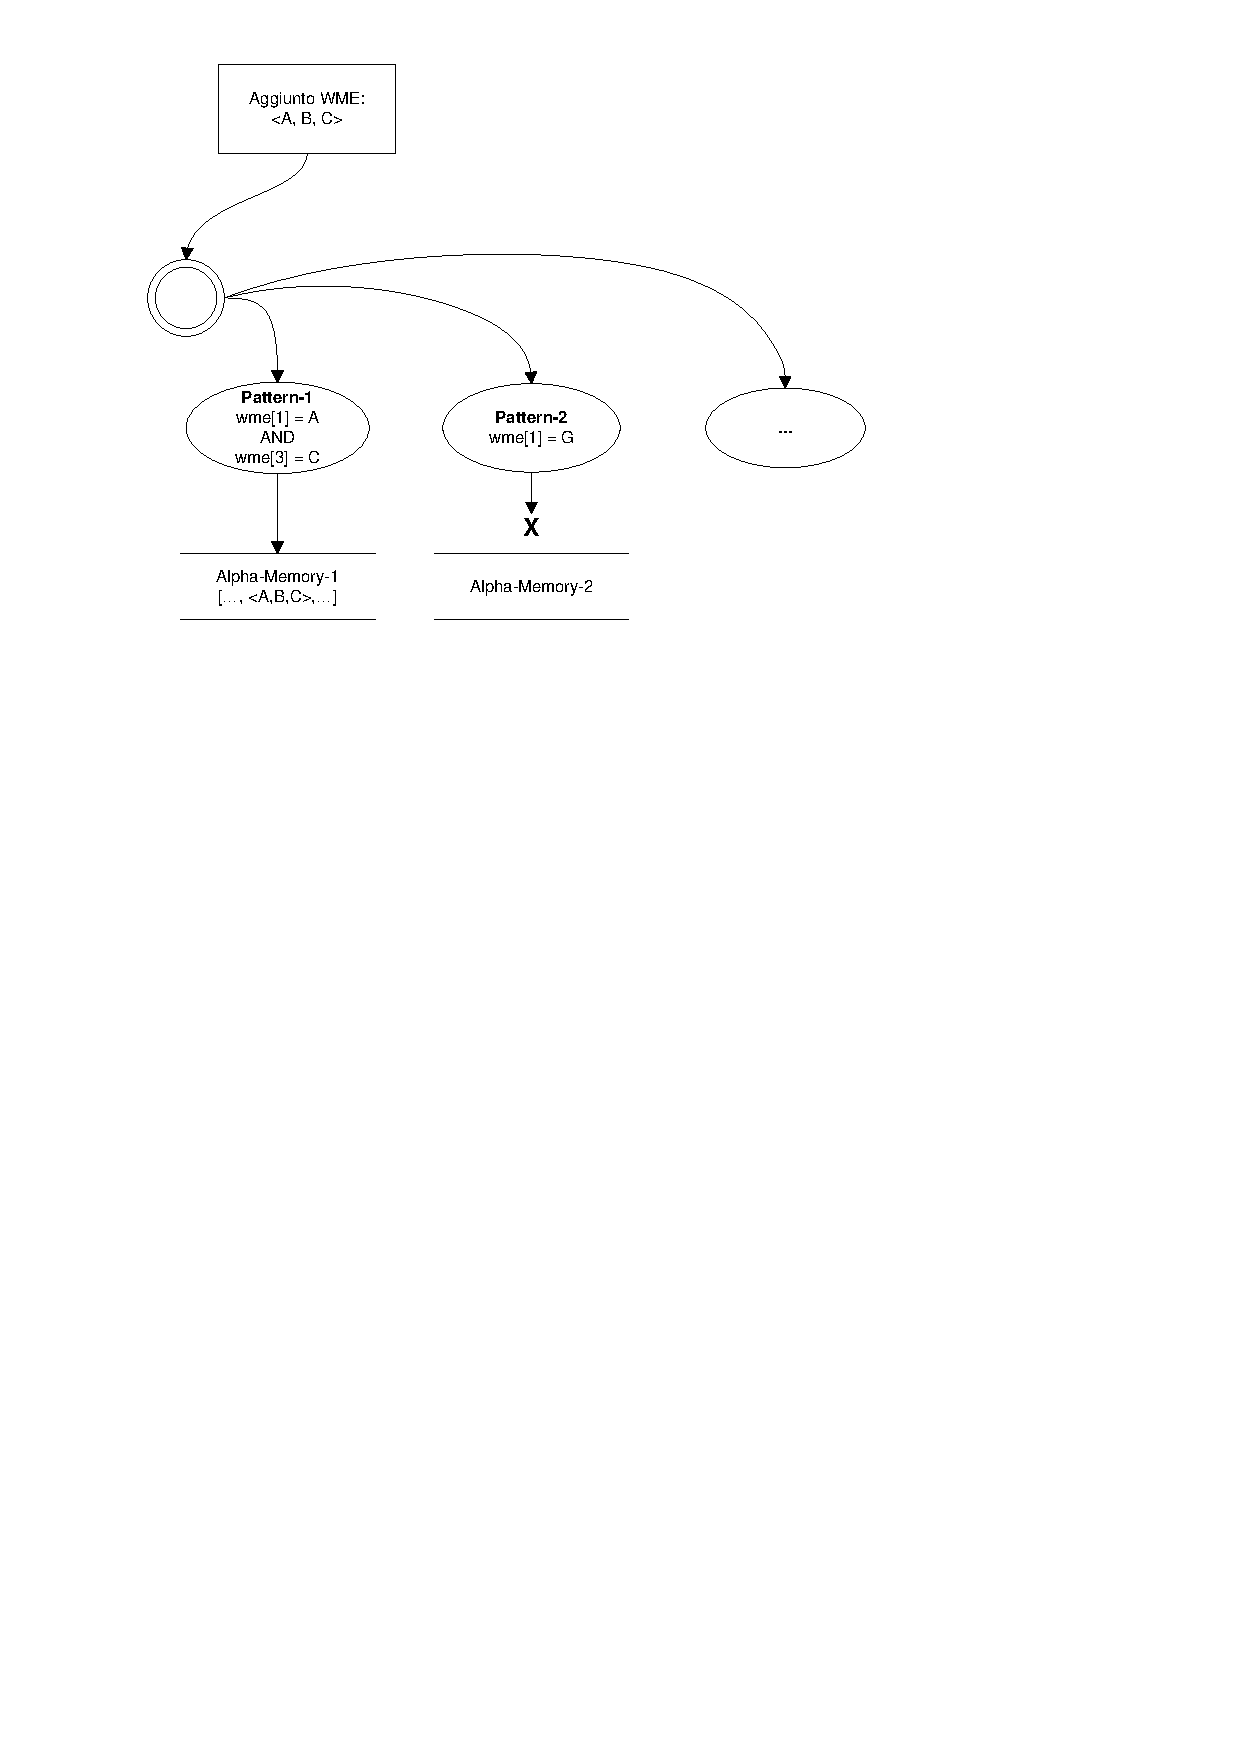
\includegraphics[viewport=70 545 416 812]{Immagini/Capitolo1/Asserzione.pdf}
\caption{Asserzione di un nuovo elemento della \emph{working memory} e valutazione tramite algoritmo RETE}\label{fig:asserzione}
\end{figure}

Quando un nuovo elemento viene asserito (\figurename~\ref{fig:asserzione}), e quindi entra a far parte della descrizione dello stato fornita dalla \emph{working memory}, l'algoritmo esegue una valutazione di ogni pattern singolarmente per il nuovo elemento aggiunto, e solo in caso di verifica positiva l'elemento stesso viene inserito all'interno dell'unità di memoria locale~\cite{forgy1982}.

Quando un elemento fuoriesce dalla \emph{working memory}, lo stesso viene rimosso da tutte le unità di memoria locali dei pattern in cui l'elemento è memorizzato. Il processo di ricerca può avvenire ripetendo nuovamente le verifiche per i singoli pattern~\cite{forgy1982} oppure, più efficientemente, tenendo in una porzione di memoria separata una lista di collegamenti fra elementi e le memorie in cui essi sono contenuti.~\cite{Doorenbos95productionmatching}

La scansione dell'intero \emph{rules-set} viene evitata attraverso l'utilizzo di una struttura a grafo per la rappresentazione delle regole. In seguito ad una fase di compilazione (\figurename~\ref{fig:grafo-regola}), la porzione \emph{LHS} delle regole viene scomposta nei singoli pattern. Per ognuno di essi viene realizzata, qualora non fosse possibile condividere una struttura analoga creata precedentemente, un circuito di nodi in grado di eseguire dei test su singoli elementi della \emph{working memory}. Come ultimo elemento del circuito viene aggiunta un'unità di memoria locale, denominata \emph{Alpha-Memory}, la quale accoglierà l'insieme di elementi che, singolarmente, hanno verificato l'elenco di condizioni che il circuito descrive~\cite{Doorenbos95productionmatching}.
L'insieme di circuiti derivanti dalla compilazione dei singoli pattern prende il nome di \emph{Alpha-Network}.

Una seconda porzione della rete è quella nota con il nome di \emph{Beta-Network}. In questa sezione vengono eseguiti i test di coerenza sul binding delle variabili fra le condizioni. Durante la fase di compilazione, una volta create le porzioni \emph{alpha} di ogni singolo pattern, quelli appartenenti alla stessa \emph{LSH} vengono collegati fra loro attraverso l'uso di speciali nodi, chiamati \emph{Join-Node}. Questi nodi, oltre a riunire singoli pattern in una catena che rappresenti l'intera \emph{LHS}, hanno il compito di eseguire l'insieme di test necessari alle verifiche di coerenza sul valore delle variabili, dove necessario. Qualora i test eseguiti in questi nodi a due input risultassero positivi, verrebbe creata una struttura contenente i due elementi della memoria di lavoro che sono risultati coerenti e la stessa memorizzata all'interno di una unità di memoria agganciata direttamente al \emph{Join-Node}. 
La struttura prende il nome di \emph{Token}\footnote{Nella formulazione dell'algoritmo proposto originariamente in \cite{forgy1979} e \cite{forgy1982} con il termine \emph{Token} si faceva riferimento a una descrizione di un cambiamento nella \emph{working memory}, notificato ai nodi componenti la rete tramite l'uso di \emph{tag}. La formulazione proposta in \cite{Doorenbos95productionmatching} utilizza l'appellativo per indicare una sequenza di \emph{working memory elements} che abbiano verificato una porzione della \emph{beta-network}. Il concetto di tag, usati nella prima formulazione per indicare il tipo di modifica che il \emph{token} rappresentava, nella seconda formulazione è completamente assente}.

\begin{figure}
\centering
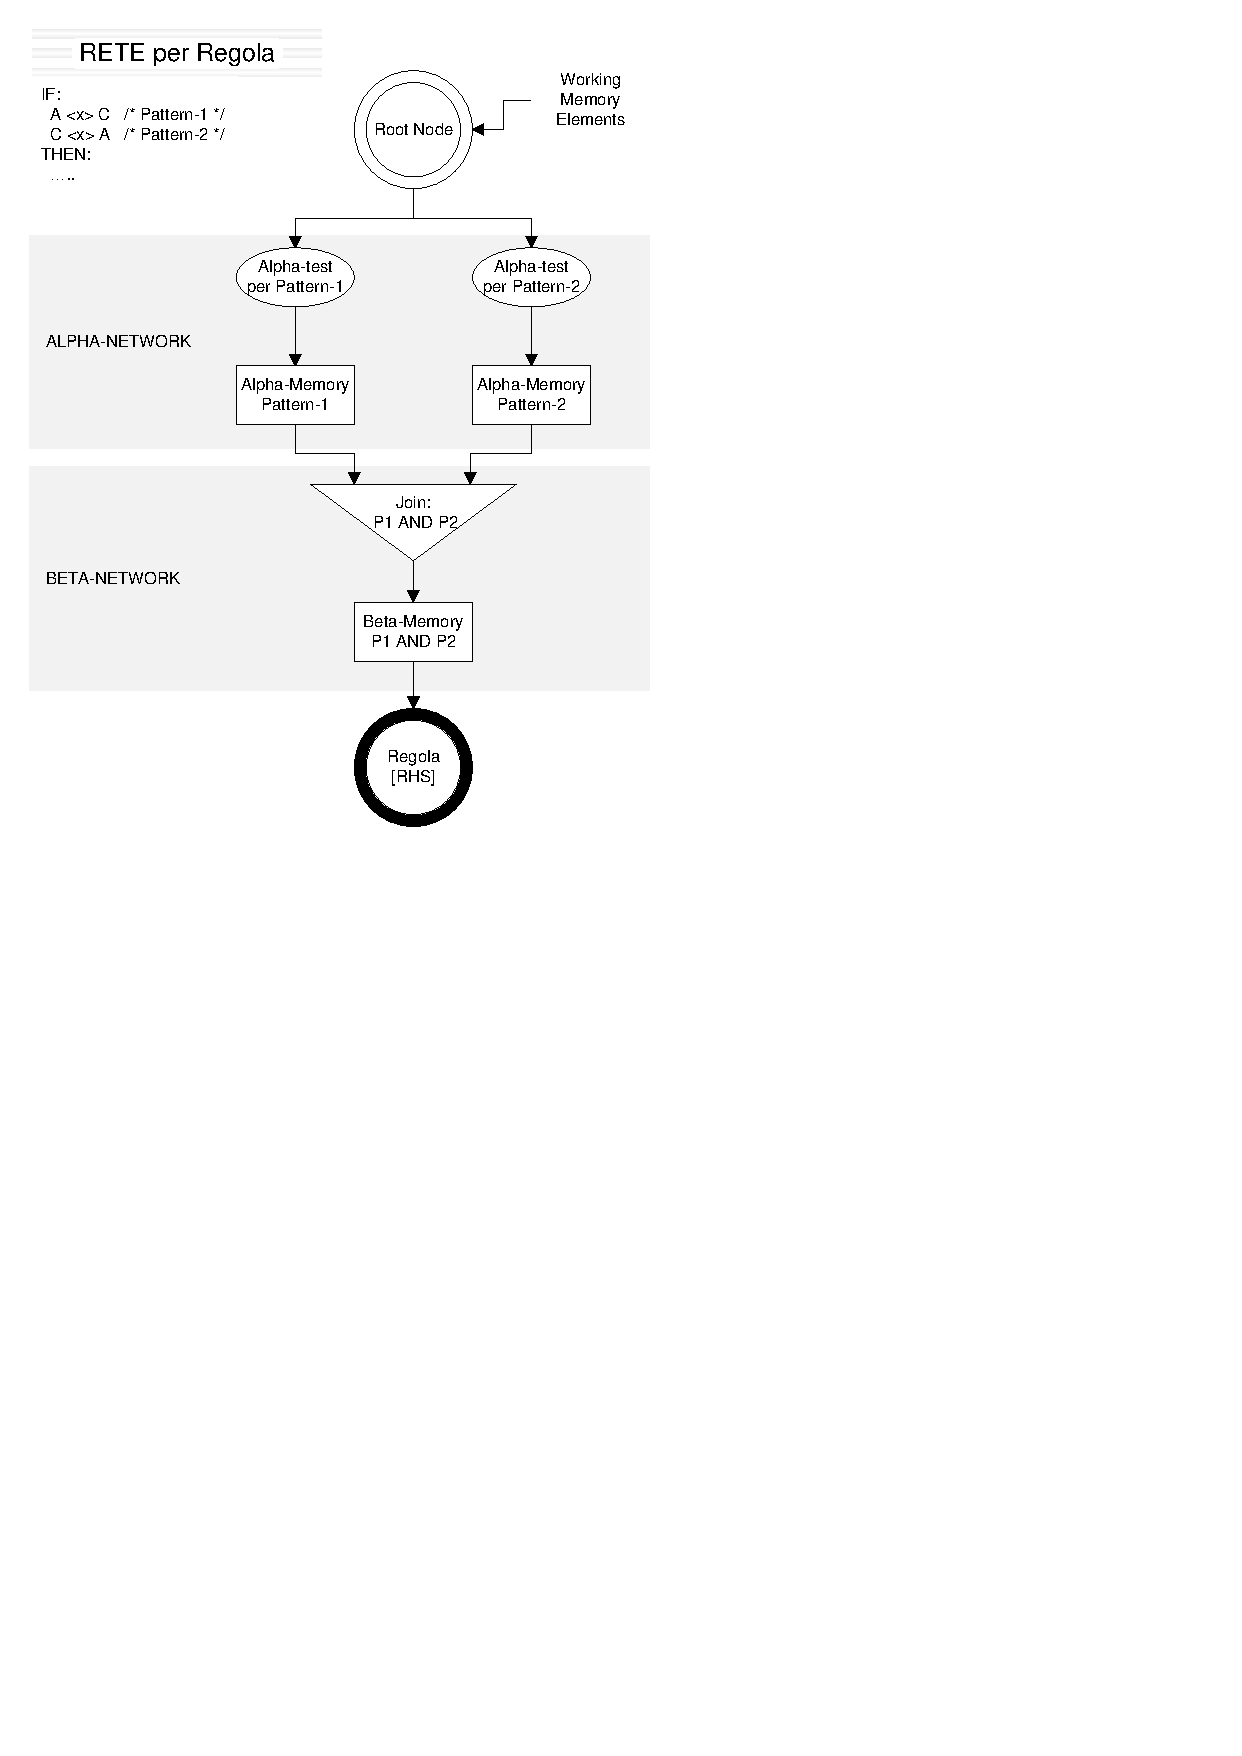
\includegraphics[viewport=14 446 312 829]{Immagini/Capitolo1/RETE-Regola.pdf}
\caption[Grafo esplicito di RETE per una regola]{Rappresentazione esplicita del grafo ottenuto dalla compilazione di una regola: vengono creati circuiti alpha per ogni \emph{pattern} e in seguito congiunti valutando la coerenza del valore della variabile $x$ fra i riscontri.}\label{fig:grafo-regola}
\end{figure}

L'utilizzo di un ulteriore tipo di memoria nella \emph{Beta-Network}, chiamata \emph{Beta-Memory}, consente di memorizzare attivazioni parziali che risultano valide solo per una porzione della regola, in attesa, che tramite l'asserzione di ulteriori fatti, l'intera regola risulti attivabile.

Il processo di trasformazione delle regole porta a due benefici sostanziali:
\begin{itemize}
	\item la compilazione dei singoli pattern eseguita per la formazione dell'\emph{alpha-network} consente di partizionare la working-memory in frammenti di minori dimensioni. Questo si traduce in un minor numero di confronti durante i test di coerenza. Inoltre, pattern simili presenti in più regole vengono accorpati e rappresentati da un unico circuito \emph{alpha}. La fase di valutazione verrà eseguita soltanto una volta per tipo di pattern.
	\item gruppi di pattern simili, analogamente a quanto descritto nel punto precedente, vengono accorpati in un solo circuito \emph{beta}, riducendo ulteriormente i costi delle verifiche per i test di coerenza.
\end{itemize}

Il processo di creazione della rete può avvenire attraverso un reale processo di compilazione \cite{forgy1982} che prevede la conversione dell'intero \emph{rules-set} in una sequenza di istruzioni ed espressioni che rappresentino le varie condizioni (implementazione \emph{compilata}), oppure attraverso un processo di creazione di una rappresentazione esplicita di grafo nelle modalità citate poc'anzi (implementazione \emph{interpretata}). 

Il vantaggio della prima variante è la maggiore velocità, che contrasta tuttavia con un maggior consumo di memoria e maggiore difficoltà di implementare procedure che, attraverso l'aggiunta o la rimozione di produzioni durante l'esecuzione, siano in grado di alterare la struttura della rete~\cite{Doorenbos95productionmatching}.
La seconda variante rende più semplice l'implementazione di procedure di manipolazione della rete e risulta globalmente di più facile implementazione e comprensione. Purtroppo questi vantaggi prevedono uno scambio di tipo prestazionale~\cite{Doorenbos95productionmatching}.

\section{Strumenti di sviluppo}

%%%%%%%%%%%%% VALUTARE RIORGANIZZAZIONE %%%%%%%%%%%%%%%%%

Tutti gli strumenti di sviluppo per sistemi esperti sono orientati a supportare la creazione di \emph{prototipi}. Un prototipo rappresenta un modello funzionante le cui funzionalità sono equivalenti ad una porzione ridotta di quelle del prodotto finale~\cite{jackson1999}.
L'idea è quella di sviluppare, nelle prime fasi del progetto, dei ''\emph{proof of concept}'' che possano essere valutati e criticati da esperti e utenti e che siano in grado di risolvere parti del problema. Questa attività è utilizzata soprattutto come un'opportunità per definire meglio requisiti e individuare criticità, verificando inoltre l'effettiva trattabilità di problematiche prima di effettuare investimenti eccessivi.

Una possibilità è che gli artefatti prodotti vengano quindi scartati al termine delle valutazioni, ma gli approcci verificati con la produzione dei prototipi stessi vengono conservati e riapplicati durante la fare di sviluppo reale del prodotto. Altre modalità prevedono l'accorpamento e sviluppo incrementale delle funzionalità del prodotto finale tramite fasi reiterate di produzione di \emph{protitipi} e valutazione.

Il numero di ambienti di sviluppo per sistemi esperti è cresciuto negli anni e con esso il numero e la tipologia di funzionalità offerte.
L'evoluzione di questi sistemi è stata motivata con il tempo e la quantità di sforzo richiesto per la costruzione di sistemi esperti.

Lo sviluppo si è focalizzato in molte aree di interesse, spaziando dall'ambito delle modalità di rappresentazione della conoscenza a quello dei meccanismi di inferenza, dallo sviluppo di regimi di controllo alla ricerca nell'ambito dei linguaggi di specifica. Indipendentemente dalle modalità con le quali è stato tentato il miglioramento, lo slancio evolutivo era ad ogni modo focalizzato nell'ambito di:
\begin{itemize}
	\item ridurre tempi e costi di sviluppo dei sistemi esperti
	\item migliorare l'affidabilità e la qualità generale dei sistemi prodotti
	\item focalizzare le attività delle varie figure professionali interessate nello sviluppo negli ambiti di propria competenza.
	\item separare le attività di analisi della conoscenza da quelle legate allo sviluppo del prodotto.
	\item fornire strumenti per velocizzare e migliorare le attività di acquisizione e aggiornamento della conoscenza.
\end{itemize}

I miglioramenti hanno incrementato in questo modo le possibilità di successo nello sviluppo di sistemi esperti. Come ulteriore effetto, il ridursi della complessità generale delle operazioni di realizzazione ha consentito di gestire e produrre soluzioni di sempre maggiore complessità.

\subsection{L'evoluzione degli strumenti di sviluppo}

Tornando indietro agli albori della produzione di sistemi esperti, i meccanismi di inferenza e le basi di conoscenza erano accoppiati fra loro. La prima generazione di sistemi non erano altro che grandi applicazioni scritte in linguaggi come LISP~\cite{knowbel1993}.

Nonostante tutti i linguaggi di programmazione potessero essere utilizzati per la produzione di sistemi esperti, alcuni di essi offrivano caratteristiche che rendevano tale attività più agevole. Rientrano in questa categoria linguaggi largamente utilizzati nelle prime fasi come il LISP e Prolog.
Purtroppo, la quantità di tempo e sforzo richiesto per la produzione usando queste tipologie di linguaggi diventava rapidamente insostenibile con l'aumentare della complessità. Inoltre, l'accoppiamento fra le funzionalità necessarie all'inferenza e quelle per la rappresentazione e la gestione della conoscenza non permetteva una distinzione di ruoli fra gli ingegneri di sistema e quelli della conoscenza~\cite{development1993}.

Questo approccio alla lavorazione venne superato nella successiva generazione. Durante la creazione di sistemi di seconda generazione come MYCIN, i ricercatori si accorsero dell'importanza di implementare i sistemi in modo che fosse possibile una separazione fra la base di conoscenza e i meccanismi che realizzavano il ragionamento.

Rimuovendo la conoscenza di dominio da questi sistemi vennero realizzati i primi sistemi di tipo \emph{Skeletal Shell}: utilizzando gli strumenti sviluppati nel progetto originale e inserendo nuova conoscenza di dominio era possibile creare una grande verità di nuovi sistemi esperti con un sforzo relativamente ridotto. I sistemi di seconda generazione di maggior successo hanno dato vita a \emph{Shell} per lo sviluppo di sistemi esperti. Ne sono esempi EMYCIN, KAS e EXPERT: rispettivamente prodotti rimuovendo le conoscenze di dominio da MYCIN, PROSPECTOR e CASNET.
Sebbene l'utilizzo di questi strumenti velocizzasse la produzione di nuovi sistemi di diversi ordini di grandezza, la necessità di attenersi alle strategie utilizzate nei sistemi originali rappresentava un limite alla flessibilità del sistema ed ai possibili ambiti di utilizzo (\figurename~\ref{fig:classificazione-tools}). 

\begin{figure}
\centering
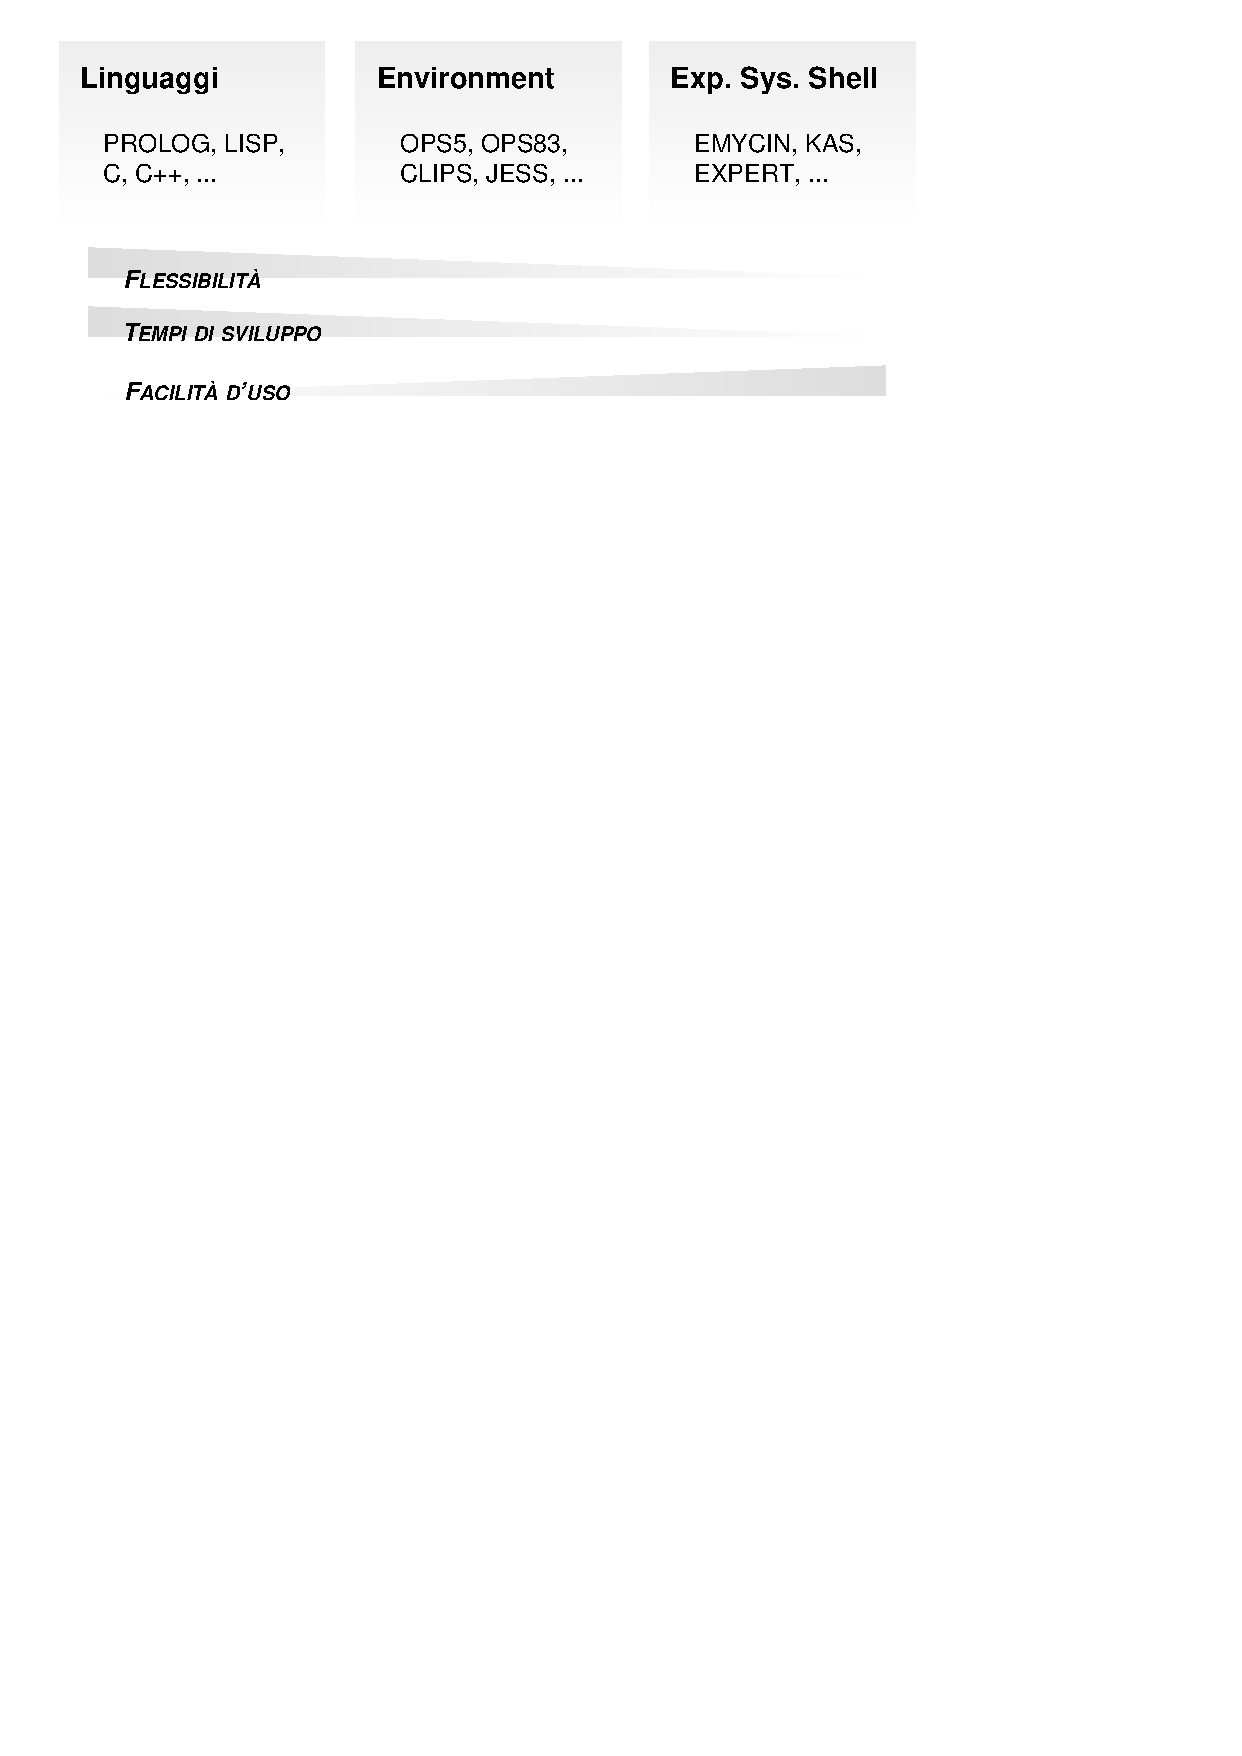
\includegraphics[width=0.9\textwidth, viewport=28 650 440 824]{Immagini/Capitolo1/Classificazione-tools.pdf}
\caption{Classificazione degli strumenti di sviluppo per sistemi esperti}\label{fig:classificazione-tools}
\end{figure}

Il successivo passo evolutivo fu compiuto con l'introduzione di linguaggi di alto livello orientati alla realizzazione di sistemi esperti e gli ambienti di programmazione multi-paradigmatici.
I primi, introdotti nella seconda metà degli anni '70, consentivano grande flessibilità e permettevano di svolgere attività di prototipazione rapida. Queste caratteristiche si traducevano nella possibilità di sperimentare  e valutare soluzioni progettuali con costi e tempi relativamente contenuti. Inoltre, per la natura stessa degli strumenti, il codice prodotto poteva essere testato in maniera incrementale durante la scrittura (possibilità offerta dal fatto che le interfacce \emph{runtime} e \emph{buildtime} erano prossime fra loro)~\cite{jackson1999}.

Spesso, questo tipo di \emph{shell} limitava la propria offerta ad un particolare tipo di formalismo per la rappresentazione della conoscenza oppure un particolare regime di controllo. La flessibilità offerta dai linguaggi di alto livello risiedeva proprio nella possibilità, per il progettista, di accedere ad approcci differenti e in questo modo spaziare fra meccanismi multipli.

Gli ambienti di programmazione multi-paradigmatici o \emph{Expert System Environment} accoppiavano la filosofia alla base dei linguaggi di alto livello con la possibilità di usufruire di differenti modalità di rappresentazione della conoscenza, regimi di controllo e paradigmi di programmazione in base alle esigenze.
Questo genere di strumenti permetteva ai programmatori di selezionare e combinare differenti moduli software. In assenza di un singolo linguaggio di rappresentazione della conoscenza che fosse valido per ogni applicazione, la soluzione era quella di fornire e rendere disponibile più di uno schema contemporaneamente.

\begin{quote}
''Sebbene non ci sia una teoria ben articolata sui sistemi basati su approccio ibrido, l'esperienza con schemi di rappresentazione e inferenza differenti ha mostrato che ognuno ha le sue debolezze; quindi la strategia di miscelare gli schemi tenta di giocare il più possibile con i loro punti di forza.''~\cite{jackson1999}
\end{quote}

\begin{figure}[h]
\centering
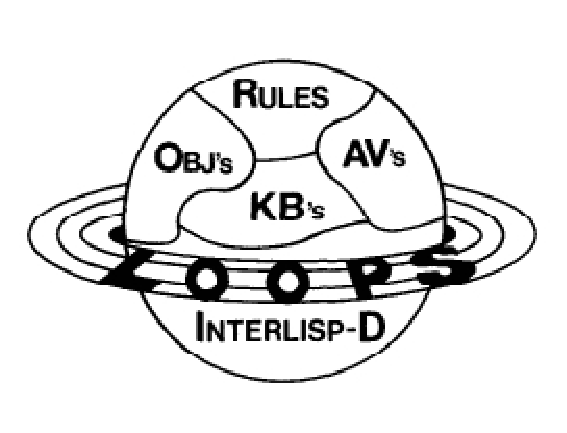
\includegraphics[scale=0.7, viewport=0 0 272 184]{Immagini/Capitolo1/LOOPS-logo.pdf}
\caption[Il logo di LOOPS]{Il logo di LOOPS: illustra i differenti paradigmi disponibili nell'\emph{environment}. Immagine originale tratta da~\cite{loops1983aaai}.}\label{fig:logo-LOOPS}
\end{figure}

Il primo esempio di ambiente multi-paradigmatico a quattro schemi fu LOOPS~(1983, \figurename~\ref{fig:logo-LOOPS}): fondeva insieme quattro paradigmi di programmazione (procedurale, basata su regole, orientata agli oggetti, orientata ai dati) all'interno di un'architettura basata sullo scambio di messaggi~\cite{loops1983aaai}.

\subsection{Skeletal Shell}
Le \emph{Shell} avevano l'obiettivo di consentire, anche a persone senza una esperienza specifica di programmazione tradizionale, di utilizzare gli sforzi compiuti da altri nell'ambito della soluzione di problematiche simili.
Fu chiaro però che l'applicabilità dell'architettura di base non era di tipo universale, sebbene consentisse di realizzare sistemi in ambiti simili a quelli per il quale il progetto era concepito.

\begin{quotation}
''EMYCIN è progettato per aiutare la costruzione e l'esecuzione di programmi che forniscono consigli. [$\dots$]

EMYCIN non è progettato per essere un linguaggio di rappresentazione \emph{general-purpose}. \`E completamente inadatto per alcuni problemi. Le limitazioni derivano in gran parte dal fatto che EMYCIN ha scelto un solo metodo per rappresentazione della conoscenza che fosse basilare, semplice da leggere e interpretare: regole di produzione applicate tramite un regime di controllo basato sul \emph{backward-chaining}~[$\dots$]''~\cite{puff1982}
\end{quotation}

Un esempio risiede in EMYCIN: sebbene consentisse di utilizzare l'architettura alla base di MYCIN e applicarla anche ad altri domini specifici nell'ambito medico (PUFF~\cite{puff1982}) o in altri ambiti (SACON~\cite{bennett1979}), la sua architettura non era abbastanza generalizzata per essere definita \emph{general-purpose}~\cite{vanmelle1984}. Era tuttavia valido per sviluppare sistemi basati sull'uso di un approccio deduttivo a problemi diagnostici, dove è disponibile una grande quantità di conoscenza ed è possibile individuare e definire le categorie diagnostiche in anticipo.

A discapito dei vantaggi in termini di semplicità nella rappresentazione della conoscenza e della specifica del sistema offerti dai tool di tipo \emph{Skeletal Shell}, le più grandi critiche a questa classe di sistemi risiedono in tre punti principali~\cite{Aikins1983163}:

\begin{itemize}
	\item[(1)] Il formalismo basato solo su regole, che la grande maggioranza di questa classe di sistemi offriva, rendeva difficile la distinzione fra conoscenza di tipo euristico, quella di controllo e quella adibita alla valutazione dei parametri richiesti. Questa limitazione rendeva difficile la comprensione dei sistemi.
	\item[(2)] L'aggiornamento e l'aggiunta di nuova conoscenza in questi sistemi rendeva difficile effettuare previsioni sull'impatto che le modifiche avrebbero avuto sul sistema nella sua interezza.
	\item[(3)] La scelta di un preciso regime di controllo spesso si adattava bene ad alcune attività, mentre rendeva difficoltoso lo sviluppo di componenti differenti dello stesso sistema (ad esempio, il regime basato su \emph{backward-chaining} offerto da EMYCIN rendeva da una parte agevole il processo di diagnosi, ma dall'altra ardua la realizzazione delle dinamiche di spiegazione).
\end{itemize}

\subsection{Expert System Environment}
Le \emph{Shell} di tipo \emph{general-purpose} offrono un maggiore controllo e flessibilità rispetto alle \emph{Skeletal Shell} rimuovendo diversi vincoli, ma questa ritrovata flessibilità viene pagata con maggiori oneri a carico dei progettisti. 

Strumenti dotati di maggiore flessibilità offrivano solo meccanismi di rappresentazione e \emph{problem-solving} basilari. Questo li rendeva adatti a qualsiasi ambito e problematica, ma il basso livello di sofisticazione obbligava gli ingegneri della conoscenza a specificare personalmente parte dei meccanismi di ragionamento e di rappresentazione. Esempi di questa sottoclasse di strumenti sono ROSIE, OPS5 e Prolog\footnote{Sebbene il Prolog sia un linguaggio di programmazione logica general-purpose, la disponibilità di meccanismi di ragionamento basilari basati su un regime di tipo \emph{backward-chaining} e la forma dichiarativa del linguaggio che rende agevole la rappresentazione della conoscenza lo rendono ascrivibile anche alla categoria delle \emph{General-Purpose Shell}}.

Maggiore semplicità era quella offerta invece dai sistemi come BLOBS, G2 o CubiCal~\cite{development1993}. Il loro ambito di utilizzo veniva ridotto, ma il maggiore livello di sofisticazione nelle forme ragionamento, unito alla disponibilità di paradigmi multipli per la rappresentazione della conoscenza, rendeva più agevole lo sviluppo di sistemi esperti. Inoltre agli ingegneri della conoscenza era richiesta una minore conoscenza delle dinamiche del sistema di base. La modifica dei meccanismi di ragionamento era ancora possibile, anche se non obbligatoria.

Gli strumenti posti al più alto grado di sofisticazione nella categoria degli \emph{environment} erano progettati per affrontare più aree di problemi. Offrivano paradigmi multipli per la specifica della conoscenza e del ragionamento, uniti a caratteristiche e utilità orientate allo sviluppo dei sistemi esperti ed alla riduzione dei tempi di iterazione nei processi di prototipazione. 

La presenza di interpreti già integrati e di paradigmi multipli di rappresentazione rendevano estremamente ridotto il carico degli ingegneri della conoscenza nella definizione dei nuovi sistemi. Nonostante tutto, la scelta di utilizzare alcune di queste funzionalità portava ad influenzare fortemente il design nei casi in cui i paradigmi offerti non corrispondessero perfettamente ai requisiti~\cite{development1993}.

\subsubsection[ART]{ART (Automated Reasoning Tool)}
ART è uno dei primi strumenti di sviluppo per sistemi esperti scritti in LISP. Offriva strutture come oggetti, regole di produzione, meccanismi per il mantenimento della catena di verità ed integrava un paradigma di programmazione orientato agli oggetti~\cite{art1998}.

\subsubsection[ART-IM]{ART-IM (ART for Information Management)}
ART-IM è una re-implementazione del sistema ART in linguaggio C, basato su una versione proprietaria dell'algoritmo RETE per la realizzazione di un regime di tipo \emph{forward-chaining} e un meccanismo di mantenimento della verità (già presente in ART).

Nonostante l'implementazione fosse fortemente incentrata sul motore inferenziale di tipo \emph{forward}, il sistema permetteva anche ragionamento basato sulla concatenazione all'indietro. L'utilizzo del regime alternativo era però sottoposto alla necessità di una specifica esplicita di strutture di controllo, alla definizione di priorità e obiettivi.

Una caratteristica importante introdotta nella re-implementazione in C era la possibilità di integrare funzionalità aggiuntive tramite lo sviluppo di funzioni separate, sempre in linguaggio C, ed integrabili durante la compilazione del sistema.

L'utilizzo di questa caratteristica ha permesso la realizzazione di ulteriori varianti (come ART-Ada~\cite{artadanasa1990}, per l'utilizzo nella specifica dei sistemi tramite linguaggio ADA), rese disponibili in seguito.

La grande varietà di funzionalità e le potenzialità offerte dal sistema nella sua interezza lo rendevano però uno strumento non adatto a progettisti alle prime armi: era richiesta conoscenza dei linguaggi C e LISP oltre che del paradigma di sviluppo orientato agli oggetti~\cite{development1993}.

\subsubsection[CLIPS]{CLIPS (C Language Integrated Production System)}

CLIPS è un \emph{environment} sviluppato al NASA Johnson Space Center nella metà del 1980. Prende spunto da tool come OPS5 e ART, supportandone le caratteristiche di maggior importanza e introducendone di nuove come le funzionalità relative alla programmazione procedurale. 

La sintassi utilizzata per lo sviluppo dei sistemi esperti è simile a quella del linguaggio LISP. 

Lo sviluppo iniziò in un contesto in cui erano emergenti, ma ancora costose, soluzioni di environment basati su linguaggio C. Il risultato è il sistema meno costoso e di maggiore reperibilità al mondo, non meno efficiente di soluzioni commerciali. La prima versione non integrava funzionalità chiave introdotte solo successivamente, come il linguaggio procedurale e il paradigma di programmazione ad oggetti~\cite{jackson1999}.

Il sistema è liberamente utilizzabile per uso personale ed accademico, mentre l'uso commerciale è soggetto all'acquisto di una licenza personale \emph{una tantum}.

Lo sviluppo del progetto, attualmente affidato ad una sola persona, è ancora in atto. Il codice sorgente è disponibile pubblicamente, cosi come le versioni compilate.

Le prime versioni di CLIPS (poco più che prototipi, implementazioni \emph{clean-room} di caratteristiche di ART)~\cite{clipsarch1992}, utilizzavano un motore basato su una implementazione dell'algoritmo RETE con regime \emph{forward-chaining} e specifica nella forma di regole di produzione. 

Il successo del progetto prima come \emph{training-tool}, poi come reale ambiente di sviluppo e distribuzione di sistemi esperti, ha giustificato lo sviluppo di versioni successive. Il progetto è stato esteso con l'integrazione del paradigma procedurale e ad oggetti (COOL).

Il successo di CLIPS è attestato dal grande numero utilizzatori: una stima realizzata nel 1992 indicava che fosse superiore a 3000, senza contare l'adozione all'interno del laboratori NASA, l'utilizzo in ambito militare, governativo, accademico e commerciale\footnote{Il numero di download del sistema dalla piattaforma di distribuzione ufficiale negli ultimi 4 anni ha superato quota 200.000. Non sono presenti misurazioni nel periodo precedente al Gennaio 2008.}~\cite{clipsarch1992}.

Negli anni sono state derivate dal progetto originale diverse varianti che espandevano specifiche categorie di caratteristiche. Alcuni esempi sono ECLiPSe~\cite{haley1991}, eCLIPS~\cite{eclips} e FuzzyCLIPS~\cite{fuzzyclips}.

\subsubsection[JESS]{JESS (Java Expert System Shell)}
Nato originariamente come un clone di CLIPS, JESS è un \emph{environment} completamente scritto in Java con l'obiettivo di integrare le funzionalità offerte da CLIPS con tecnologie per il web basate su Java. 
Le prime versioni offrivano il supporto ad un set limitato delle caratteristiche di CLIPS. Con il tempo lo sviluppo si è diretto verso l'aggiunta di funzionalità originali in maniera indipendente dal progetto padre, separando in questo modo i due progetti~\cite{laerhoven1999}~\cite{jessfaq}~\cite{jessmanual}.

Sebbene JESS non integri un linguaggio di specifica di tipo \emph{object-oriented}, la forte integrazione con il linguaggio Java con cui è implementato consente di utilizzare particolari notazioni, gli \emph{shadow-fact}, per collegare elementi nella \emph{working-memory} con istanze di classi specificate in linguaggio Java.


\subsection{Il problema dell'integrazione}

Molti degli strumenti originariamente progettati per lo sviluppo di sistemi esperti stand-alone non supportavano l'integrazione con altri componenti software di utilizzo comune come database o fogli di calcolo.
A volte i linguaggi, o le piattaforme, scelti per l'implementazione di questi sistemi erano un freno alle possibilità di integrazione. I primi strumenti basati sul linguaggio LISP richiedevano apparecchiature appositamente sviluppate (\emph{LISP-machines}) e grandi quantitativi di memoria. Questo si traduceva, oltre che nella richiesta di grandi investimenti, anche in architetture fortemente specializzate. Il grande costo di queste apparecchiature limitava anche le possibilità di diffusione e successo dei prodotti sviluppati con questi tool~\cite{development1993}.
Questi strumenti basati su LISP introducevano anche grossi problemi in termini di portabilità degli artefatti prodotti~\cite{clipsarch1992}.

Per superare questi ostacoli, molti dei tool originariamente sviluppati in LISP vennero con il tempo riscritti per essere utilizzati su piattaforme emergenti di più grande diffusione (come le workstation e le piattaforme convenzionali che utilizzavano Unix come sistema operativo prima, o i Personal Computer poi).
Durante questo processo di conversione, la scelta di molti ricadde verso il linguaggio C, molto diffuso e supportato da tutte le piattaforme. L'adozione del C portò ad un incremento prestazionale dei sistemi oltre ad offrire nuovi scenari in cui sperimentare l'integrazione fra il software disponibile sulle nuove piattaforme e gli strumenti di sviluppo per sistemi esperti.
Prendendo in esame CLIPS, il sistema poteva essere integrato all'interno di qualsiasi applicazione che fosse in grado di interfacciarsi direttamente con librerie scritte in linguaggio C. JESS estende ulteriormente queste possibilità tramite l'utilizzo di Java, linguaggio emergente negli ultimi anni sia in ambiente \emph{coorporate} che nei prodotti di largo consumo.

Studi effettuati negli ultimi anni hanno analizzato l'efficienza, la facilità e le possibilità offerte dallo sviluppo di software con vari linguaggi di programmazione~\cite{naiditch1999}~\cite{Zeigler_95}~\cite{prechelt2000}~\cite{prashant2008}.
Sebbene questi studi abbiamo mostrato, come prevedibile, che le caratteristiche di particolari linguaggi si adattino meglio ad alcuni ambiti di utilizzo rispetto che ad altri, un elemento comune emerso riguarda l'impatto che la scelta del linguaggio ha sui costi di sviluppo e l'affidabilità degli artefatti prodotti. Nonostante la grande flessibilità offerta dal linguaggio C, i costi affrontati per lo sviluppo, il testing e la manutenzione degli artefatti prodotti erano superiori rispetto a quelli imposti da altri linguaggi come Ada~\cite{Zeigler_95}, Java~\cite{prashant2008} o a linguaggi interpretati come Perl o Python\cite{prechelt2000}.

\section{Obiettivi di questa tesi}
Negli ultimi anni Internet, e più specificamente il \emph{World Wide Web}, sta evolvendo da un medium per lo scambio di informazioni verso una piattaforma onnipresente per la distribuzione di qualsiasi genere di servizi come \emph{Web banking}, \emph{E-Commerce}, \emph{E-Government}, etc. La ragione alla base di questa rapida evoluzione del Web è il grande numero di possibilità che questa forma di distribuzione offre, unito al grande successo che questo genere di soluzioni sta riscontrando verso l'utenza.

L'orientamento verso il calcolo distribuito, lo stoccaggio di dati personali tramite servizi \emph{cloud-based}, la conversione del consumo classico verso declinazioni digitali, sono tutti frammenti di questa evoluzione.

In questo ambito, la possibilità di integrazione delle tecnologie classiche per la realizzazione di sistemi esperti con strumenti di nuova generazione orientati allo sviluppo per il web offre molti spunti per la ricerca nell'ambito degli \emph{expert system environment}. L'approfondimento delle tematiche relative allo sviluppo di nuove soluzioni rappresenta uno spunto per capire in maniera più intima le dinamiche alla base del funzionamento dei sistemi esperti e degli strumenti che ne consentono la creazione e la distribuzione.

%Unire problematiche tanto differenti all'interno di un solo strumento richiede la progettazione di soluzioni flessibili.

%%%%%%%%%%%% UNIRE UN CAPOVERSO PER INDICARE I FINI DIDATTICI %%%%%%%%%%%%%%%

Lo scenario di riferimento descritto nell'arco di questo capitolo, unito alle problematiche emergenti dallo sviluppo orientato al Web, è la base su cui si vuole proporre un \emph{environment per sistemi esperti} flessibile e che consenta un'integrazione rapida con tecnologie esistenti orientate al web.

Gli obiettivi perseguiti nell'ambito di questa tesi sono riassumibili come segue:
\begin{itemize}
	\item fornire un \emph{expert system environment} dotato di una architettura flessibile in grado di permettere l'aggiunta di nuove caratteristiche;
	\item estendere il sistema prodotto con funzionalità che consentano la distribuzione dei servizi offerti dall'\emph{environment} anche attraverso un modello d'architettura di tipo \emph{client-server}, che agevoli la creazione di soluzioni basate su calcolo distribuito.
\end{itemize}




\chapter{Analisi del sistema}

Lo scopo di questo capitolo è quello di fornire un'analisi del sistema da proporre. Verrà specificato il contesto nel quale l'artefatto dovrà operare, mettendo in evidenzia, in seguito ad una analisi preliminare, l'insieme dei requisiti che dovranno risultare soddisfatti. Per la struttura di questo capitolo verranno utilizzate, come riferimenti, le specifiche suggerite in \cite{ieee830-1998}.

\section{Scopo del sistema}

Il progetto \emph{MyCLIPS} si prefigge lo scopo di sviluppare un software di tipo \emph{Expert System Environment}, mediante la realizzazione di un ambiente multi-paradigmatico che supporti programmazione procedurale e basata su regole, un regime di controllo di tipo \emph{forward chaining} e che fornisca soluzioni per la distribuzione dei servizi tramite architettura \emph{client-server}.

L'artefatto derivante dall'implementazione del progetto \emph{MyCLIPS} non sarà un prodotto con fini commerciali, ma piuttosto uno strumento di supporto alla ricerca nell'ambito degli \emph{environment per sistemi esperti} e dell'integrazione degli stessi con tecnologie orientate al web.

\section{Definizioni, acronimi, abbreviazioni}

\begin{itemize}
	\item \emph{Ambiente di sviluppo integrato}:
	\item \emph{Analisi dei requisiti}:
	\item \emph{API}:
	\item \emph{Best Practice}:
	\item \emph{Bug}:
	\item \emph{C}:	
	\item \emph{Client}:
	\item \emph{Casi d'uso}:
	\item \emph{Codice sorgente}:
	\item \emph{CPU}:
	\item \emph{Design Pattern}:
	\item \emph{Eclipse}:
	\item \emph{Expert System Environment}:
	\item \emph{Forward Chaining}:
	\item \emph{GUI}:
	\item \emph{IDE}:
	\item \emph{Incapsulamento}:
	\item \emph{Incrementale}:
	\item \emph{Java}:
	\item \emph{Javadoc}:
	\item \emph{Multipiattaforma}:
	\item \emph{MyCLIPS}:
	\item \emph{Open source}:
	\item \emph{Overhead}:
	\item \emph{Package}:
	\item \emph{Pattern Matching}:
	\item \emph{Plugin}:
	\item \emph{PyDev}:
	\item \emph{Python}:
	\item \emph{RETE}:
	\item \emph{Strategia di risoluzione dei conflitti}:
	\item \emph{Rule-Based Systems}:
	\item \emph{Server}:
	\item \emph{Sistema Operativo}:
	\item \emph{Skeleton}:
	\item \emph{Standalone}:
	\item \emph{Stub}:
	\item \emph{Thread}:
	\item \emph{UML}:
	\item \emph{Unificazione}:
	\item \emph{Use Case}:
	\item \emph{XML}:
	\item \emph{XMLRPC}:
\end{itemize}

\section{Riferimenti teorici}

In questa sezione si forniscono dei riferimenti a basi teoriche necessarie per la comprensione del problema che il progetto punta a risolvere.


\subsection{Rule-Based Systems}

I sistemi di produzione sono un tipo di \emph{Pattern Directed Inference System}. Rappresentano un modello computazionale con regime di controllo guidato da \emph{pattern}. 

Il processo decisionale viene guidato attraverso l'utilizzo di regole: strutture costituite da coppie \emph{antecedente-conseguente}.

La parte \emph{antecedente}, definita anche \emph{LHS} o \emph{condizione}, contiene la rappresentazione di uno schema di caratteristiche che devono corrispondere nella descrizione dello stato corrente del sistema. Nel caso questi schemi (\emph{pattern}) risulteranno verificati, la regola verrà definita \emph{attivabile}. L'attivazione della regola non è immediata, ma gestita in un flusso di controllo ben prestabilito. Con il termine \emph{attivazione} verrà definita la coppia formata da una \emph{regola attivabile} e l'insieme di caratteristiche presenti nella descrizione dello stato che hanno reso la regola \emph{attivabile}.

La parte \emph{conseguente}, definita anche \emph{RHS} o \emph{azione}, rappresenta l'azione (o l'insieme di azioni) che dovranno essere eseguite nel momento in cui una regola \emph{attivabile} verrà effettivamente attivata. Solitamente il gruppo conseguente consiste in una serie di modifiche da apportare alla descrizione dello stato del sistema, ma questa generalizzazione non rappresenta una restrizione.

Il funzionamento di questa classe di sistemi può essere espresso come una sequenza di cicli \emph{recognize-act}:
\begin{description}
	\item[recognize:] viene valutata l'applicabilità di ogni regola in relazione allo stato corrente del sistema. La valutazione viene effettuata confrontando lo stato del sistema con la porzione \emph{LHS} di ogni regola.
	\item[selezione:] vengono applicati dei principi di selezione per individuare una o più regole fra quelle attivabili. L'insieme di principi utilizzati viene definito con il nome di \emph{strategia di risoluzione di conflitti}.
	\item[act:] la regola selezionata viene attivata: l'elenco di azioni presenti nella porzione \emph{RHS} vengono eseguite.
\end{description}

\'E evidente come il ciclo sia strutturato in modo che il momento di esame dei dati sia nettamente separato dal momento di elaborazione o modifica degli stessi. Inoltre l'unica modalità per lo scambio di informazioni fra le regole prevista, avviene attraverso la modifica stessa dello stato del sistema presente nella \emph{working memory}. Questa caratteristica differenzia ulteriormente questa classe di sistemi da quelli con approccio procedurale: se l'approccio basato su regole di produzione prevede che la stessa descrizione dello stato sia condivisa fra tutte le regole e che l'accesso allo stesso sia garantito in egual misura, il modello procedurale prevede che le singole procedure accedano ad un ristretto (e focalizzato) sottoinsieme dei dati presenti nello stato globale.

\subsubsection{Componenti di un RBS}


La struttura classica di un sistema basato su regole può essere schematizzata (\figurename~\ref{fig:architettura-rbs}) attraverso la specifica dei quattro componenti principali da cui è composto.

\begin{figure}[h]
\centering
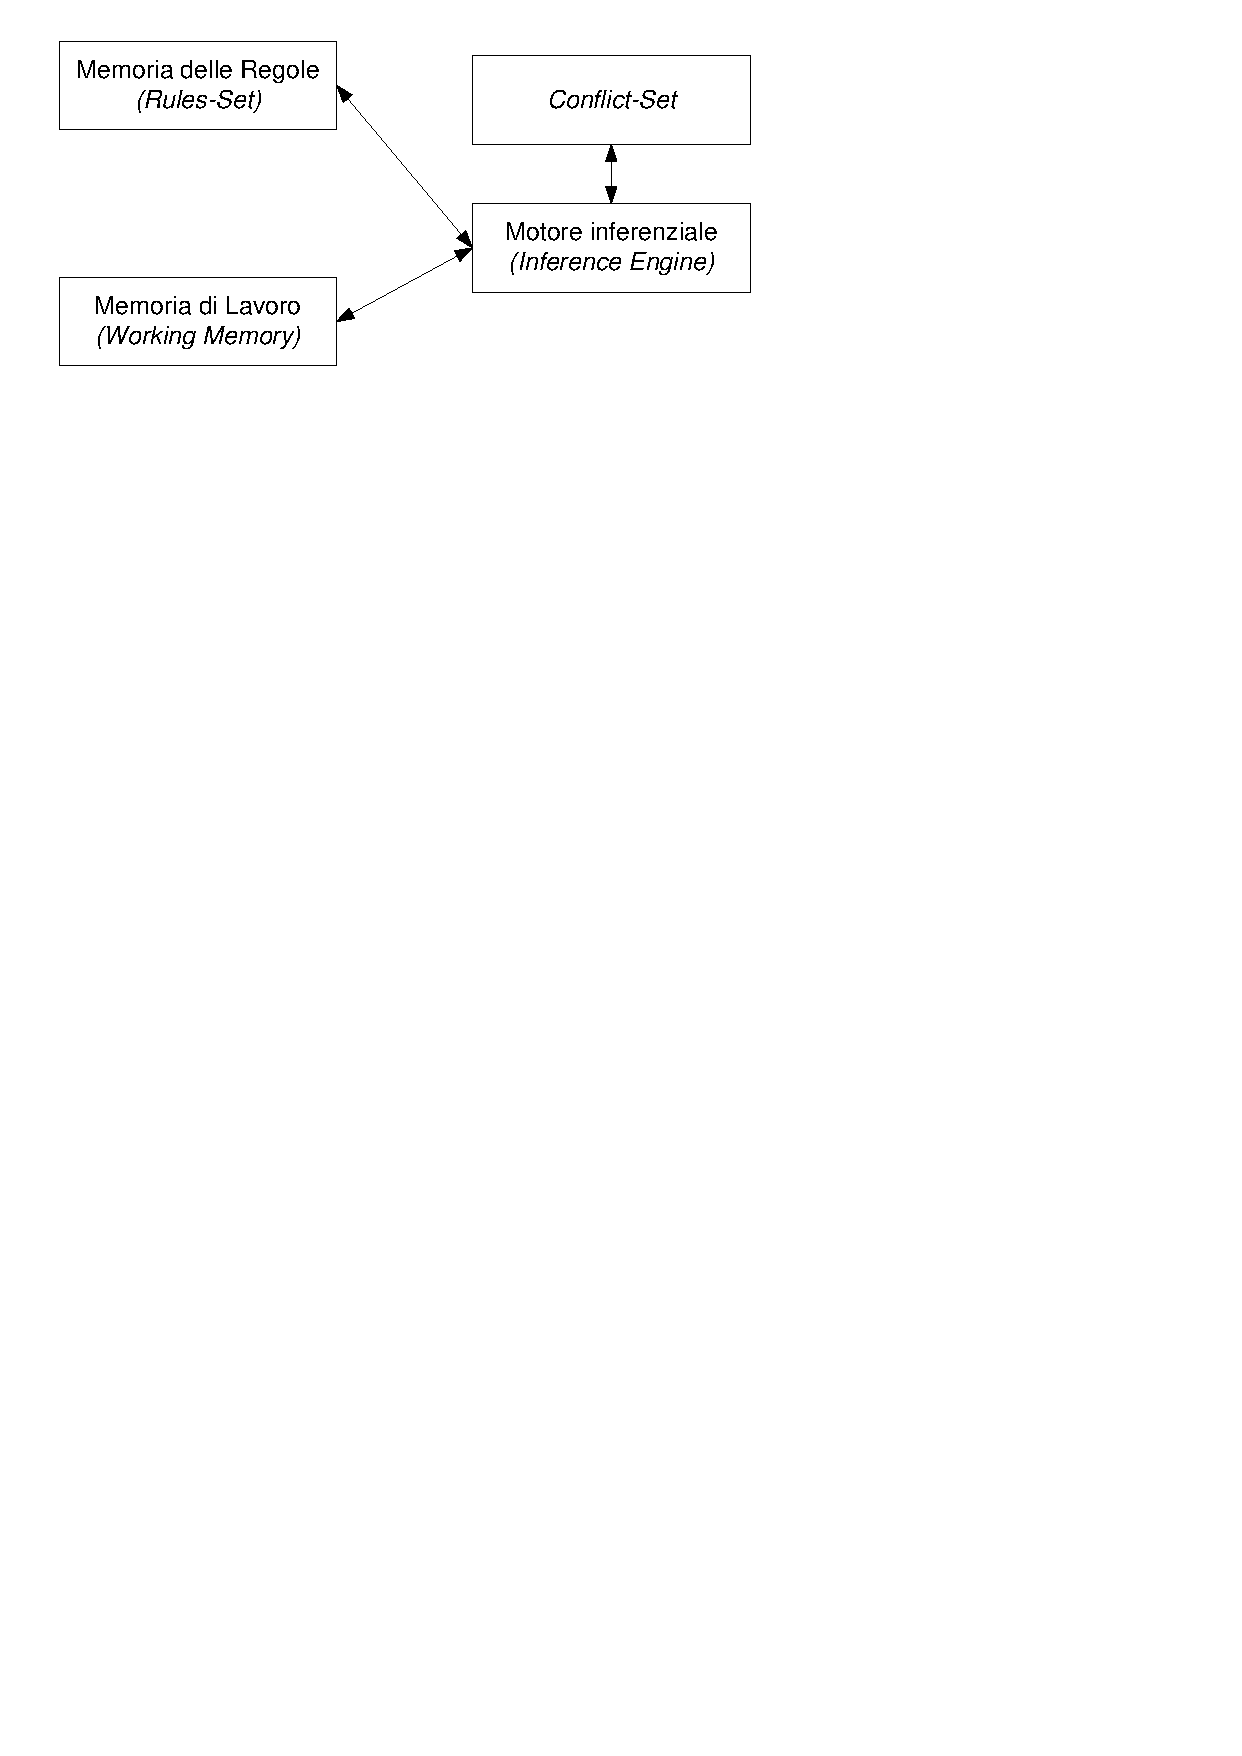
\includegraphics[viewport=28 667 361 824]{Immagini/Capitolo2/Architettura-RBS.pdf}
\caption{Architettura generalizzata di un Rule-Based System}\label{fig:architettura-rbs}
\end{figure}

\subparagraph{Memoria di lavoro}
La memoria di lavoro, anche chiamata \emph{working memory}, è il componente destinato ad accogliere la descrizione simbolica dello stato del sistema. La descrizione è composta da strutture simboliche note con il nome di \emph{fatti}. La forma con la quale i fatti vengono rappresentati dipende dal sistema spesso, ma formalismi comunemente utilizzati prevedono una rappresentazione tramite \emph{vettori di caratteristiche} o \emph{triple (oggetto, proprietà, valore)}.

La \emph{working memory} viene utilizzata dal motore inferenziale per il processo di verifica della possibilità di attivazione delle regole.

\subparagraph{Motore inferenziale}

Il \emph{motore inferenziale}, o \emph{inference engine}, rappresenta il nucleo centrale di ogni sistema a regole: è il componente con il compito di valutare la parte \emph{LHS} delle regole, identificare quelle attivabili compilando il \emph{conflict-set} e infine, in seguito ad un processo di selezione guidato dalla \emph{strategia di risoluzione dei conflitti}, eseguirne una.

Il processo alla base della valutazione delle regole applicabili prende il nome di \emph{pattern-matching}.

\subparagraph{Memoria delle regole}
La memoria delle regole, o \emph{rules-set}, è una struttura che conserva l'insieme di regole definite nel sistema. Viene consultata dal motore inferenziale per individuare le regole attivabili per uno stato del sistema.

\subparagraph{Conflict-Set}
Il \emph{conflict-set}, anche noto in determinati sistemi con il nome di \emph{agenda} o \emph{agenda delle attivazioni}, è un componente che conserva l'insieme di \emph{attivazioni} disponibili per lo stato corrente della \emph{working-memory}. L'insieme viene compilato dal \emph{motore inferenziale} al termine del passo \emph{recognize} che caratterizza questa classe di sistemi.

Il \emph{conflict-set} viene consultato per effettuare una selezione nell'insieme di attivazioni disponibili, utilizzando una \emph{strategia di risoluzione dei conflitti}, e individuare l'attivazione da eseguire nel passo \emph{act}.

\subsection{Unificazione e Pattern Matching}\label{par:pattern-matching}

Il problema del \emph{confronto di descrizioni simboliche} è uno dei problemi alla base dei sistemi basati su conoscenza. Una forma di questo genere di problemi è quello dell'\emph{unificazione} o \emph{matching}.

L'\emph{unificazione} rappresenta un procedimento con il quale vengono confrontate fra loro un insieme di due o più strutture simboliche per identificarne differenze o somiglianze.~\cite{ferilli200}

Dati due termini $s$ e $t$, il problema dell'unificazione consiste nel capire se esistono dei termini in grado di essere sostituiti alle variabili che compaiono in $s$ e $t$ affinché i termini ottenuti risultino identici.~\cite{ferilli200}

Per molte applicazioni pratiche, l'unificazione risulta un concetto troppo generale. Si fa quindi riferimento al \emph{Pattern Marching}, una variante dell'unificazione nella quale è possibile effettuare sostituzioni solo in una delle due strutture simboliche.~\cite{ferilli200}


\begin{defn}[Termini confrontabili]
Dati due termini, $s$ e $t$, si dice che \emph{esiste un matching} tra essi se esiste una sostituzione $\mu$ tale che:
\begin{equation}
\mu(s)=t \text{ oppure } \mu(t)=s
\end{equation}
In tal caso $\mu$ è definito \emph{matcher} di $s$ e $t$, mentre $\mu(s)$ (risp. $\mu(t)$) è definito \emph{matching} di $s$ e $t$.
\end{defn}

\subsection{Strategie di risoluzione dei conflitti}\label{par:strategies}

Come visto in precedenza, la fase \emph{recognize} ha lo scopo di valutare eventuali cambiamenti apportati allo stato del sistema identificando l'insieme di \emph{attivazioni} disponibili. L'elenco di \emph{attivazioni} verrà memorizzato nel \emph{conflict-set}. 

In una fase successiva, l'utilizzo di determinate euristiche provvederà a definire dei criteri con i quali discriminare l'insieme di attivazioni per identificarne un sotto-insieme\footnote{Solitamente composto di un solo elemento.}.

L'insieme di criteri con i quali discriminare l'insieme prende il nome di \emph{strategia di risoluzione dei conflitti}.

\subsection{CLIPS}\label{par:clips}

CLIPS (C Language Integrated Production System) è uno dei più conosciuti \emph{Expert System Environment}. Implementato in linguaggio C presso i laboratori NASA del Johnson Space Center, è attualmente uno dei sistemi più utilizzati in ambito accademico grazie alla sua reperibilità e gratuità.

CLIPS è un ambiente multi-paradigmatico che integra all'interno di un'architettura di base di tipo \emph{RBS}, elementi per la programmazione procedurale e orientata ad oggetti.

L'interazione con il sistema può avvenire attraverso l'utilizzo di una \emph{Shell}, che consente l'immissione di costrutti, l'esecuzione di query e chiamate a funzioni, oppure attraverso l'integrazione del sistema in applicazioni classiche, che ne sfruttino i servizi tramite apposite API.

Il sistema prevede dei meccanismi di estensione tramite la compilazione congiunta di funzioni in linguaggio C, le quali verranno rese disponibili nel sistema in maniera analoga a quelle integrate in origine.

\subsubsection{Presentazione dei formalismi di specifica}\label{par:clips-formalism}

Il linguaggio di specifica utilizzato da CLIPS, prevede una sintassi simile a quella utilizzata da LISP. La definizione dei costrutti (\emph{regole}, \emph{template}, \emph{funzioni}, \emph{fatti}, $\dots$) avviene utilizzando un linguaggio chiamato CLIPS, analogamente al sistema. Un'estensione del linguaggio fornito originariamente, che prende il come di \emph{COOL}, è stata aggiunta nelle versioni successive per integrare il supporto il paradigma \emph{object-oriented}.

\paragraph{Moduli}
Per consentire il riuso e agevolare lo sviluppo incrementale dei sistemi esperti, oltre che per agevolare la specifica di meccaniche di tipo \emph{goal-directed}, CLIPS prevede la definizioni di moduli e un protocollo per la condivisione delle definizioni dei costrutti fra più moduli.

\begin{program}
\begin{verbatimtab}

(defmodule A
	(export ?ALL))

(defmodule B
	(import A ?ALL))
\end{verbatimtab}
\caption{Esempio d'uso di \emph{defmodule} per la specifica di moduli}
\end{program}

La definizione dei moduli avviene utilizzando il costrutto \emph{defmodule}. La sintassi prevede la possibilità di specificare un elenco di costrutti da rendere disponibili ad altri moduli (tramite l'attributo \emph{export}), oppure un elenco di definizioni da importare da un modulo precedentemente creato (tramite l'attributo \emph{import}).

Il meccanismo di \emph{import/export} è una delle caratteristiche principali del sistema di moduli fornito da CLIPS. Consente in questo modo di introdurre un meccanismo di \emph{information hiding} e rendere più facile in riuso di moduli indipendenti.

\paragraph{Funzioni utente}
L'utente, in maniera alternativa all'integrazione di funzioni native scritte in linguaggio C, può aggiungere funzioni personalizzate all'interno del sistema utilizzando il costrutto \emph{deffunction}.

\begin{program}
\begin{verbatimtab}

(deffunction Funzione_Di_Prova (?arg1)
	(printout t ?arg1 crlf)
)
\end{verbatimtab}
\caption{Esempio d'uso di \emph{deffunction} per la specifica di funzioni}
\end{program}


Le funzioni cosi integrate potranno essere utilizzate nelle stesse modalità previste dalle altre funzioni di sistema, con l'eccezione relativa ai vincoli di visibilità fra moduli.

\begin{program}
\begin{verbatimtab}

(defmodule A
	(export deffunction Funzione_Di_Prova))
	
(deffunction A::Funzione_Di_Prova () )

(defmodule B
	(import A deffunction Funzione_Di_Prova))
\end{verbatimtab}
\caption{Esempio di esportazione della definizione di una funzione}
\end{program}

Le definizioni di funzioni devono essere esportate dal modulo in cui sono definite e successivamente importate da quello che, invece, intende utilizzarle.

\paragraph{Regole}
Componente chiave di ogni \emph{RBS}, la specifica delle regole può essere effettuata utilizzando il costrutto \emph{defrule}.

\begin{program}
\begin{verbatimtab}

(defrule Make_Bird_Fly
	(bird (type ?X))
	=>
	(assert (bird (type ?X)	(fly yes)))
)
\end{verbatimtab}
\caption{Esempio d'uso di \emph{defrule} per la specifica di una regola}\label{code:defrule}
\end{program}

L'attivabilità della regola è soggetta, oltre che a vincoli relativi dal normale processo di \emph{pattern-matching}, anche a vincoli derivanti dal modulo in cui il processo è focalizzato.

Come mostrato in Codice~\ref{code:defrule}, la porzione \emph{LHS} e \emph{RHS} della regola sono separati dal simbolo $=>$. La regola definizione i \emph{pattern} della \emph{LHS} usando i formalismi \emph{Ordered-Fact} e \emph{Template-Fact}. I \emph{pattern} possono essere accorpati e specificati in aggiunta a modificatori come \emph{exists}, \emph{not}, \emph{or}, $\dots$.

La porzione \emph{RHS} contiene chiamate a procedure di sistema o definite dall'utente tramite il costrutto \emph{deffunction}.

\paragraph{Fatti}

I \emph{fatti}, insieme alle \emph{instanze}, costituiscono il contenuto della \emph{working memory}. L'asserzione o ritrattazione dei fatti avviene attraverso l'utilizzo della funzioni di sistema \emph{assert} e \emph{retract}. Altre funzioni che interagiscono con la \emph{memoria di lavoro} con modalità simili, ma effetti leggermente differenti, sono \emph{modify} e \emph{duplicate}.

L'utilizzo di queste funzioni avviene congiuntamente all'utilizzo di una delle due possibili notazioni per la specifica dei fatti.

\begin{program}
\begin{verbatimtab}

(deffacts Fatti_Iniziali
	(A B C)
	(bird (type penguin))
	(bird (type eagle))
	(combattente
		(mano-sx pugnale)
		(mano-dx tomahawk)
		(cintura scalpo scalpo scalpo))
)
\end{verbatimtab}
\caption{Definizione di un gruppo di fatti tramite \emph{deffacts}}\label{code:deffacts}
\end{program}


Una possibilità alternativa di specifica dei fatti iniziali è quella prevista tramite l'utilizzo del costrutto \emph{deffacts}. Il costrutto consente di inserire un elenco di definizioni che verranno automaticamente asserite durante la fase di inizializzazione del sistema esperto.

\begin{program}
\begin{verbatimtab}

(A B C)
\end{verbatimtab}
\caption{Fatto definito utilizzando la notazione \emph{Ordered-Fact}}\label{code:ordered-fact}
\end{program}

La prima, chiamata \emph{Ordered-Fact}, prevede la definizione di fatti come vettori di elementi simbolici o numerici di lunghezza definita. Il formato del primo elemento è richiesto che sia di tipo \emph{SYMBOL}\footnote{SYMBOL rappresenta un tipo elementare presente in CLIPS. Appartengono a questo tipo tutte le sequenze alfanumeriche non delimitate da apici e che abbiano come primo elemento un carattere alfabetico}, il formato dei successivi elementi è arbitrario.

\begin{program}
\begin{verbatimtab}

(combattente
	(mano-sx scudo)
	(mano-dx spada)
	(cintura carne-secca borraccia monete))
\end{verbatimtab}
\caption[Fatto definito utilizzando la notazione \emph{Template-Fact}]{Fatto definito utilizzando la notazione \emph{Template-Fact}. Il nome del template a cui il fatto fa riferimento è \emph{combattente}. La specifica del \emph{template} prevede l'esistenza degli slot ''mano-sx'', ''mano-dx'' e ''cintura''}\label{code:template-fact}
\end{program}

La seconda modalità di specifica, denominata \emph{Template-Fact}, prevede la definizione dei fatti tramite l'utilizzo di un \emph{template} e una sequenza di \emph{slot}. Gli slot rappresentano delle caratteristiche definite nella specifica di \emph{template}.
La definizione del fatto può prevedere la specifica di tutti o solo una porzione degli \emph{slot} previsti dal \emph{template}. CLIPS prevede la possibilià di definire dei valori di \emph{default} da applicare in caso di mancato avvaloramento di uno slot.
I valori inseribili negli \emph{slot} possono essere singoli elementi o multipli. Nel secondo caso si farà riferimento allo \emph{slot} con il nome di \emph{multi-slot} (un esempio è quello fornito dal \emph{multi-slot} ''cintura'' dell'esempio in Codice~\ref{code:template-fact}).

\paragraph{Template}
La specifica dei fatti in formato \emph{Template-Fact} prevede la definizione preventiva di un \emph{template} che definisca una ''tipologia'' di fatti, indicandoli con un nome univoco, e una sequenza di caratteristiche, esplicitando utilizzando \emph{slot} e \emph{multi-slot}.

\begin{program}
\begin{verbatimtab}

(deftemplate combattente "rappresenta un combattente"
	(slot mano-sx 
		(type SYMBOL))
	(slot mano-dx
		(default spada)
		(type SYMBOL))
	(multislot cintura))
\end{verbatimtab}
\caption{Specifica di \emph{Template} tramite \emph{deftemplate}}\label{code:deftemplate}
\end{program}

L'esempio fornito in Codice~\ref{code:deftemplate} rappresenta una possibile definizione di \emph{template} valida per il fatto in Codice~\ref{code:template-fact}.

La specifica prevede la definizione di valori di \emph{default} (come ad esempio per lo \emph{slot} ''mano-dx''), da attribuire nei casi in cui non venga fornito un valore durante l'asserzione, oppure di restrizioni sul tipo di valore memorizzabile nello \emph{slot}.

\subsection{Architetture per sistemi distribuiti}

Un sistema distribuito consiste di una collezione di componenti, distribuiti su diversi terminali (anche chiamati \emph{host}) connessi fra loro attraverso una rete. Questi componenti interagiscono fra loro al fine di scambiare dati od accedere reciprocamente a servizi disponibili.~\cite{Mascolo:2002:MCM:770420.770423}

Ad alto livello, la realizzazione di un sistema distribuita è soggetta alla predisposizione di un sistema di comunicazione in grado di mettere in comunicazione i processi distribuiti fra i vari \emph{host}.

Sono disponibili diverse architetture per strutturare un sistema distribuito. Le più note prendono i nomi di \emph{Client-Server}, \emph{3-tier Architecture}, \emph{n-tier Architecture}, \emph{Peer-to-Peer}, solo per citarne alcune.

\subsubsection{Modello Client-Server}
Il modello di architettura \emph{Client-Server} si basa sul partizionamento delle attività, risorse e responsabilità del sistema in due classi di componenti: \emph{Server} e \emph{Client}.

I componenti possono essere distribuiti su diversi \emph{host}, così come possono essere collocati in processi separati residenti sulla stessa macchina in modo che non condividano direttamente risorse (\figurename~\ref{fig:client-server}). Lo scambio di informazioni avviene attraverso un protocollo stabilito e noto ad entrami i sistemi.

\begin{figure}[h]
\centering
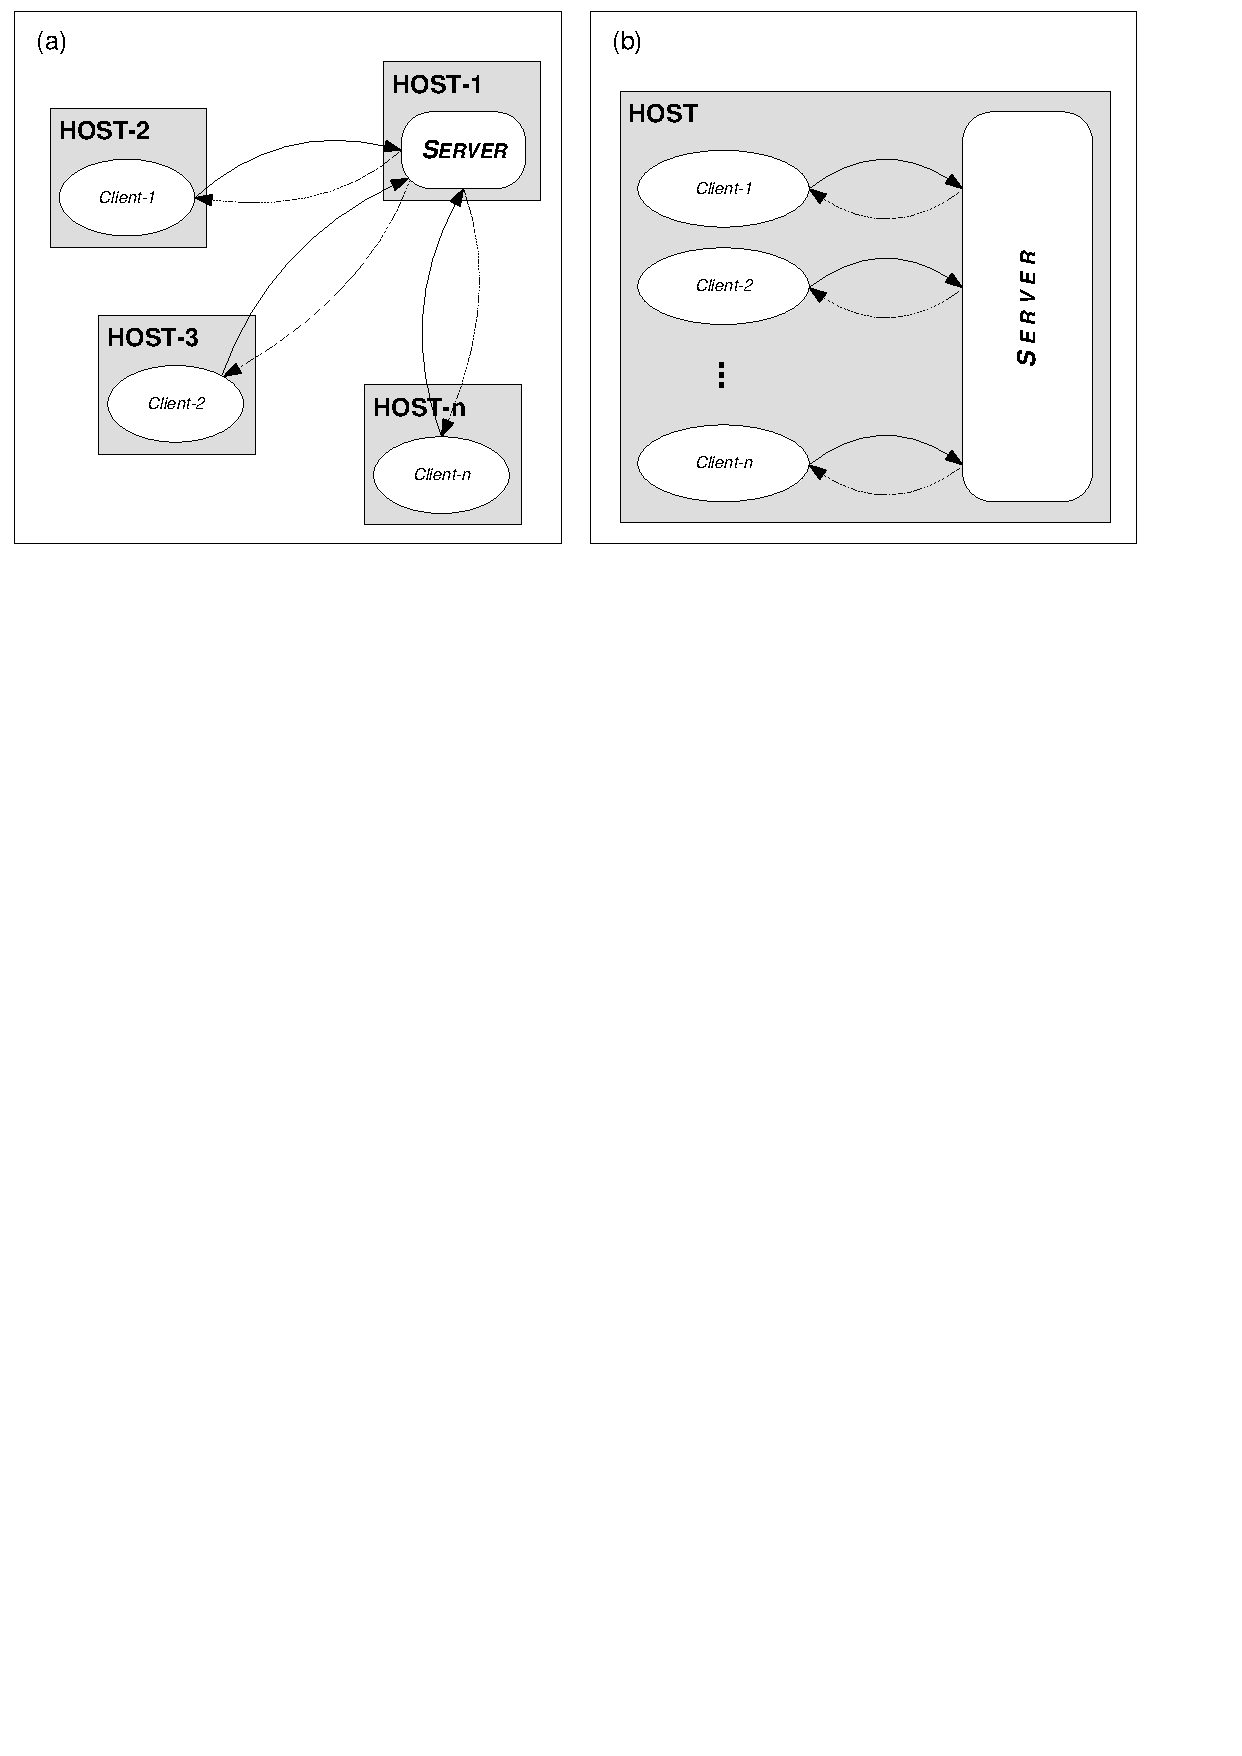
\includegraphics[scale=0.7, viewport=6 582 546 838]{Immagini/Capitolo2/Client-Server.pdf}
\caption[Architettura \emph{Client-Server}]{Architettura \emph{Client-Server}: in \emph{(a)} è mostrata una distribuzione su \emph{host} multipli, in \emph{(b)} una distribuzione in processi multipli}\label{fig:client-server}
\end{figure}

L'architettura \emph{Client-Server} descrive un modello di collaborazione fra sistemi. Il \emph{server} offre servizi o funzionalità a uno o più \emph{client}, mentre il \emph{client} effettua una richiesta e, solitamente, provvede ad elaborare i dati ottenuti come risposta dal \emph{server} per presentarli all'utente o proseguire con ulteriori elaborazioni.

\subsubsection{Protocollo XML-RPC}\label{par:xmlrpc}

\emph{Remote Procedure Call}, o \emph{RPC}, è un meccanismo tramite il quale un'applicazione posizionata su una \emph{macchina} richiede l'utilizzo di servizi forniti da un'altra applicazione residente su una \emph{macchina} differente. Con il termine \emph{macchina} non viene unicamente inteso un \emph{host}, un'installazione fisicamente indipendente, ma anche un processo residente in una porzione di memoria indipendente e che rende l'accesso alle risorse del servizio impossibile se non tramite il meccanismo \emph{RPC}. 

Il meccanismo \emph{RPC} prevede che una prima applicazione possa inviare uno o più messaggi ad una applicazione differente per invocare delle procedure. L'applicazione ricevente ha la possibilità,  a sua volta, di inviare i risultati dell'elaborazione tramite un ulteriore messaggio verso applicazione richiedente.~\cite{MERRICK:2006:misc}

\emph{RPC} descrive un meccanismo generalizzato per l'invocazione di procedure remote, non una concreta implementazione di un protocollo o di tecnologie per lo scambio dei messaggi fra gli \emph{host}. Partendo dal concetto generale di \emph{RPC}, nel tempo sono state proposte differenti implementazioni basate su protocolli proprietari o codifiche dei messaggi differenti.~\cite{JAIRATH:2004:misc}~\cite{dcerpc}

\emph{XML-RPC} è una fra le implementazioni proposte per \emph{RPC}: si propone come un meccanismo di chiamata a procedura remote semplice e versatile. Il brevetto originale con il quale è stato proposto descrive sia il meccanismo di chiamata, che un sistema per l'implementazione del metodo.~\cite{MERRICK:2006:misc}

\begin{figure}[h]
\centering
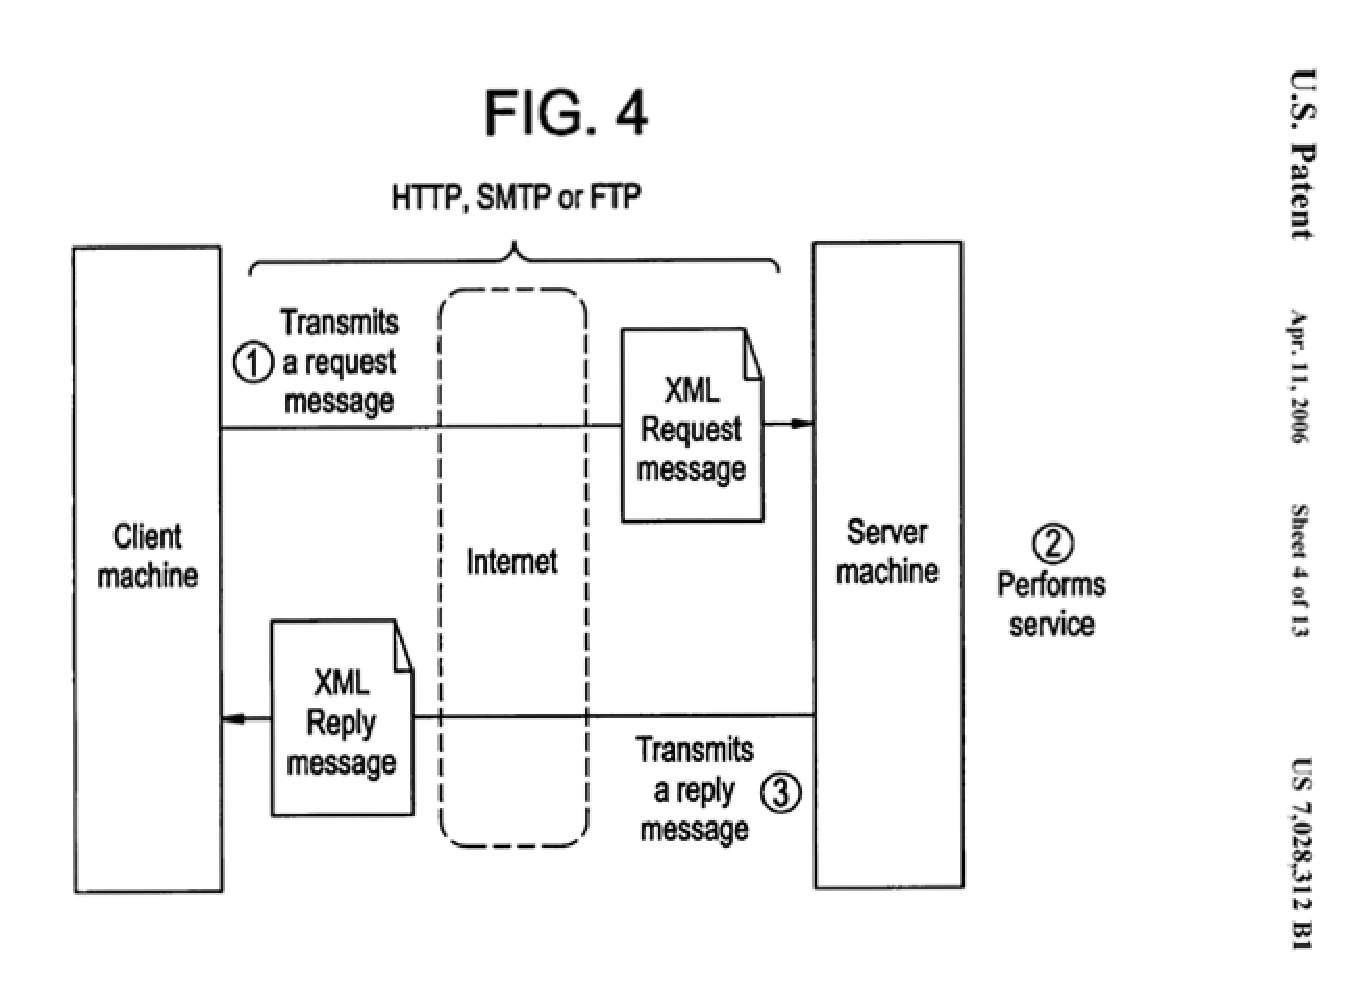
\includegraphics[scale=0.5, viewport=0 0 646 440]{Immagini/Capitolo2/XMLRPC-patent.pdf}
\caption[Comunicazione tramite \emph{XML-RPC}]{Comunicazione tramite \emph{XML-RPC}: immagine presente nella richiesta originale di brevetto~\cite{MERRICK:2006:misc}.}\label{fig:xmlrpc-patent}
\end{figure}

\emph{XML-RPC} prevede lo scambio di richieste e risposte usando il formato \emph{XML}, attraverso meccanismi di trasporto multipli. Solitamente, con l'uso del termine \emph{XML-RPC} si è soliti però indicare il protocollo di scambio messaggi in \emph{XML} attraverso un meccanismo di trasporto basato sul protocollo \emph{HTTP}.

\begin{program}
\begin{verbatimtab}

POST /RPC2 HTTP/1.0
User-Agent: Frontier/5.1.2 (WinNT)
Host: betty.userland.com
Content-Type: text/xml
Content-length: 181


<?xml version="1.0"?>
<methodCall>
   <methodName>examples.getStateName</methodName>
   <params>
      <param>
         <value><i4>41</i4></value>
         </param>
      </params>
   </methodCall>
\end{verbatimtab}
\caption{Esempio di chiamata ad una procedura remota usando \emph{XML-RPC over HTTP}}\label{code:xmlrpc-request}
\end{program}

La codifica dei messaggi viene effettuata incapsulando i parametri di chiamata ed i valori di ritorno all'interno di appositi frammenti del documento \emph{XML}, i quali hanno il compito di attribuire una semantica alla stringa rappresentante il valore.

\begin{program}
\begin{verbatimtab}
HTTP/1.1 200 OK
Connection: close
Content-Length: 158
Content-Type: text/xml
Date: Fri, 17 Jul 1998 19:55:08 GMT
Server: UserLand Frontier/5.1.2-WinNT


<?xml version="1.0"?>
<methodResponse>
   <params>
      <param>
         <value><string>South Dakota</string></value>
         </param>
      </params>
   </methodResponse>
\end{verbatimtab}
\caption{Esempio di messaggi inviato a risposta di una chiamata a procedura remota usando \emph{XML-RPC over HTTP}}\label{code:xmlrpc-response}
\end{program}

I \emph{tag} che contengono il valore ne determinano il tipo. Nell'esempio fornito in Codice~\ref{code:xmlrpc-request}, il valore ''41'' (tipo \emph{integer}) viene incapsulato nel \emph{tag i4}. Il tag indica appunto che il tipo del valore, come da specifica, è un \emph{4 bytes signed integer}.

La specifica prevede la possibilità di utilizzare un set di tipi atomici con i quali rappresentare tutti i parametri di chiamata a procedura o i valori di ritorno (''integer'', ''string'', ''boolean'', ''double'', ''dateTime.iso8601'', ''base64'') e un gruppo di strutture composte (''struct'' per strutture analoghe a dizionari, ''array'' per vettori).~\cite{xmlrpcspec}

\section{Capacità}

Si riassumono quindi le funzionalità richieste al sistema.

\begin{enumerate}
	\item l'uso di un linguaggio di specifica che consenta:
		\begin{enumerate}
			\item la definizione di regole di produzione (\ref{par:clips-formalism})
			\item l'utilizzo di un paradigma procedurale (\ref{par:clips-formalism})
			\item la specifica di funzioni utente (\ref{par:clips-formalism})
			\item la specifica di moduli (\ref{par:clips-formalism})
			\item definizione di template di fatti (\ref{par:clips-formalism})
			\item la specifica della conoscenza fattuale tramite:
				\begin{enumerate}
					\item fatti in notazione Ordered-Fact (\ref{par:clips-formalism})
					\item fatti in notazione Template-Fact (\ref{par:clips-formalism})
				\end{enumerate}
		\end{enumerate}
	\item la possibilità di aggiungere strategie di risoluzione dei conflitti (\ref{par:strategies})
	\item la possibilità di integrare nuove funzioni di sistema (\ref{par:clips})
	\item compatibilità con i sistemi sviluppati per CLIPS (\ref{par:clips})
	\item l'utilizzo dell'algoritmo RETE per le operazioni di \emph{Pattern-Matching}~(\ref{par:pattern-matching})
	\item la possibilità di accedere alle funzionalità del sistema tramite una \emph{shell}~(\ref{par:clips})
	\item la possibilità di accedere alle funzionalità del sistema tramite protocollo XML-RPC~(\ref{par:xmlrpc})
\end{enumerate}


\section{Vincoli di sistema}
\vincoliinit
\subsection{Vincoli di interfaccia}

\'E prevista l'interazione fra utente e sistema attraverso l'utilizzo di una \emph{Shell} di comandi per permettere la specifica e l'esecuzione dei sistema esperto.  A soddisfacimento della capacità richiesta 7, è previsto l'utilizzo del sistema tramite protocollo XML-RPC che consenta agli utenti di integrare le funzionalità del sistema in applicazioni di terze parti. In base a queste premesse si esplicitano i seguenti vincoli d'interfaccia.
\vincolistart
	\item Hardware\\	
	L'utente si interfaccia al sistema inserendo appositi comandi tramite tastiera. Inoltre acquisisce i risultati dell'elaborazione dei comandi attraverso il monitor. La tastiera viene inoltre utilizzata per l'inserimento di dati, qualora necessario.
	
	\item Utente\\
	L'interazione con il sistema avviene attraverso un'interfaccia testuale composta da una linea di comando, nella quale l'utente esplicita i comandi e attende i risultati dell'elaborazione. Anche i risultati vengono presentati nella medesima interfaccia testuale.
	
	\item Software\\
	L'utilizzo del sistema attraverso l'integrazione in applicazioni di terze parti (tramite integrazione diretta o interfaccia XML-RPC) prevede l'utilizzo di applicazioni per la scrittura di software o ambienti di sviluppo integrati (IDE).
	
	\item Software\\
	Il sistema prevede la possibilità di utilizzare applicazioni di \emph{text-editing} per la creazione dei sistemi esperti.
	
\vincoliend

\subsection{Vincoli operativi}

\vincolistart
	\item Hardware\\
	Per l'utilizzo in modalità servizio XML-RPC:
	\begin{itemize}
		\item 1GB di memoria RAM;
		\item Interfaccia di rete.
	\end{itemize}
	\item Software\\
	\'E previsto l'utilizzo del sistema su piattaforma PC con sistemi operativi
	\begin{itemize}
		\item Microsoft Windows XP, Vista, 7
		\item Ubuntu 12.04
	\end{itemize}
\vincoliend

\subsection{Vincoli prestazionali}
\vincolistart
	\item le prestazioni complessive del sistema devono permettere il completamento dei test di una \emph{benchmark-suite} in tempo ragionevole.
\vincoliend
\subsection{Vincoli di progetto}
\vincolistart
	\item il sistema deve permettere l'esecuzione di artefatti realizzati tramite CLIPS (escludendo quelli che utilizzano le estensioni del linguaggio COOL), richiedendo soltanto modifiche di lieve entità.
	
	\item il sistema deve prevedere la possibilità di integrare nuove funzionalità
\vincoliend

\subsection{Stabilità dei vincoli}

\begin{longtable}{|c|c|c|p{7cm}|}
\caption{Matrice di stabilità dei vincoli}\label{tab:stabilita-vincoli}\\
\hline\hline
\rowcolor{grigio-chiarissimo} \textbf{\#} & \textbf{Stabile} & \textbf{Instabile} & \textbf{Motivazione} \\
\hline\hline
\endfirsthead
\hline\hline
\rowcolor{grigio-chiarissimo} \textbf{\#} & \textbf{Stabile} & \textbf{Instabile} & \textbf{Motivazione} \\
\hline\hline
\endhead

Vincolo-1 &  & $\blacklozenge$ & Nuove tecnologie potrebbero far migrare il sistema verso nuove forme di interazione \\ 
\hline 
Vincolo-2 & $\blacklozenge$ &  &  \\ 
\hline 
Vincolo-3 & $\blacklozenge$ & & \\ 
\hline 
Vincolo-4 & $\blacklozenge$ & & \\ 
\hline 
Vincolo-5 &  & $\blacklozenge$ & Lo sviluppo tecnologico potrebbe portare a richieste hardware differenti come conseguenza di un ampliamento delle richieste software \\ 
\hline 
Vincolo-6 & $\blacklozenge$ & & \\ 
\hline 
Vincolo-7 & & $\blacklozenge$ & Lo sviluppo del sistema potrebbe portare all'introduzione di vincoli prestazionali \\ 
\hline 
Vincolo-8 & & $\blacklozenge$ & Lo sviluppo del sistema potrebbe portare all'ampliamento della compatibilità o a modifiche del linguaggio che riducano la portabilità degli artefatti\\ 
\hline 
Vincolo-9 & $\blacklozenge$ & & \\ 
\hline

\end{longtable}


\section{Attori e Casi d'uso}

\subsection{Attori}

In seguito ad un'analisi preliminare, sono state individuate sette classi di attori principali (\figurename~\ref{fig:attori}).

\begin{figure}[h]
\centering
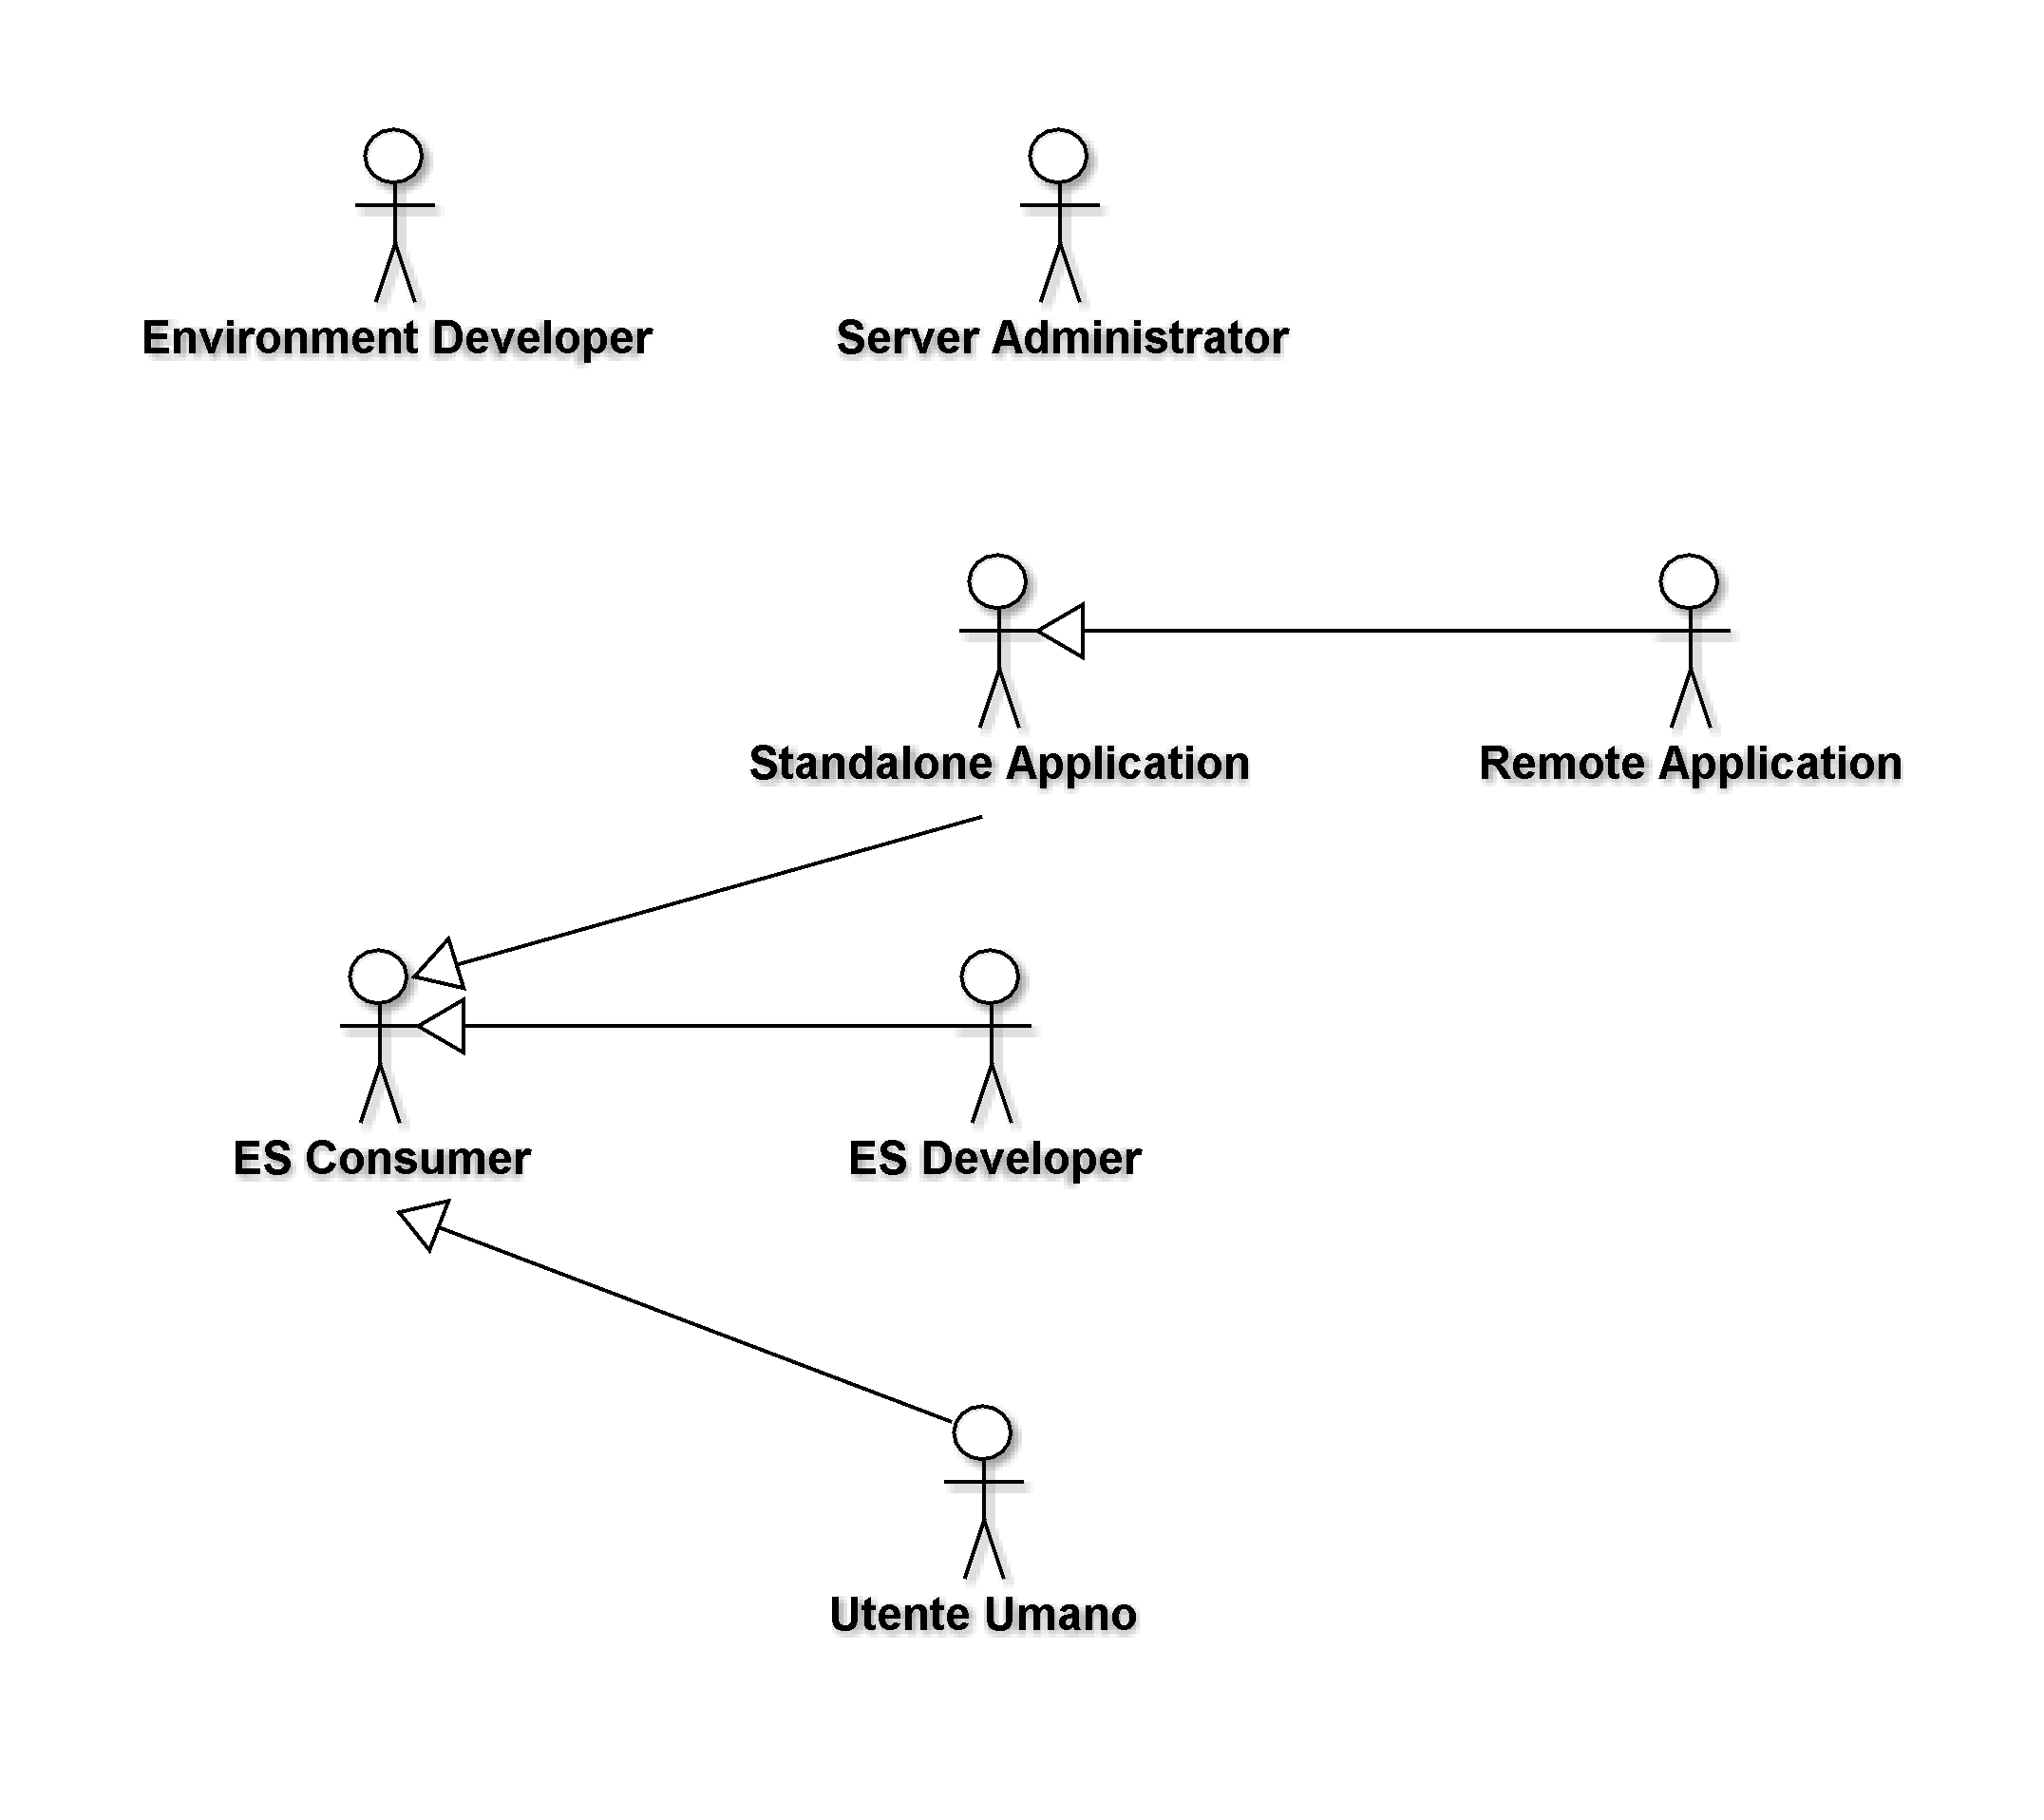
\includegraphics[width=0.9\textwidth]{Immagini/Capitolo2/UseCases/Attori.png}
\caption{Gerarchia degli attori}\label{fig:attori}
\end{figure}

\begin{description}
	\item[ES Consumer:] rappresenta un attore generalizzato in grado di utilizzare i servizi principali offerti dall'\emph{environment} per caricare, eseguire ed interagire con un artefatto precedentemente creato tramite i protocolli offerti dall'\emph{environment} stesso.
	
	\item[ES Developer:] specializzazione di \emph{ES Consumer}, servendosi del linguaggio di specifica fornito dall'\emph{environment} realizza artefatti eseguibili. Tramite l'utilizzo di apposite interfacce è anche in grado di testare l'artefatto prodotto analizzando rappresentazioni grafiche delle strutture interpretate e registri d'attività dell'esecuzione dell'artefatto.
	\item[Utente Umano:] specializzazione di \emph{ES Consumer}.
	
	\item[Standalone Application:] specializzazione di \emph{ES Consumer}. Utilizza i servizi offerti dall'\emph{environment} all'interno di applicazioni \emph{stand-alone}. Esegue artefatti e valuta i risultati dell'esecuzione analizzando eventi e lo stato finale del sistema.
	
	\item[Remote Application:] specializzazione di \emph{Standalone Application}. Esegue attività analoghe a quelle di \emph{Standalone Application}, ma utilizzando i servizi tramite appositi protocolli di comunicazione. Per supportare questi protocolli l'attore può creare, configurare o distruggere sessioni.
	
	\item[Environment Developer:] utilizzando la documentazione di sistema e le apposite \emph{API} fornite, estende le funzionalità dell'\emph{environment} aggiungendo nuove funzioni di sistema, strategie di risoluzione dei conflitti o \emph{event-listener}. Utilizzando un framework per l'esecuzione di test d'unità, può verificare il funzionamento delle funzioni integrate.
	
	\item[Server Administrator:] configura e gestisce un'istanza server dell'\emph{environment}.
	
\end{description}

\subsection{Organizzazione dei Casi d'uso}

\begin{figure}
\centering
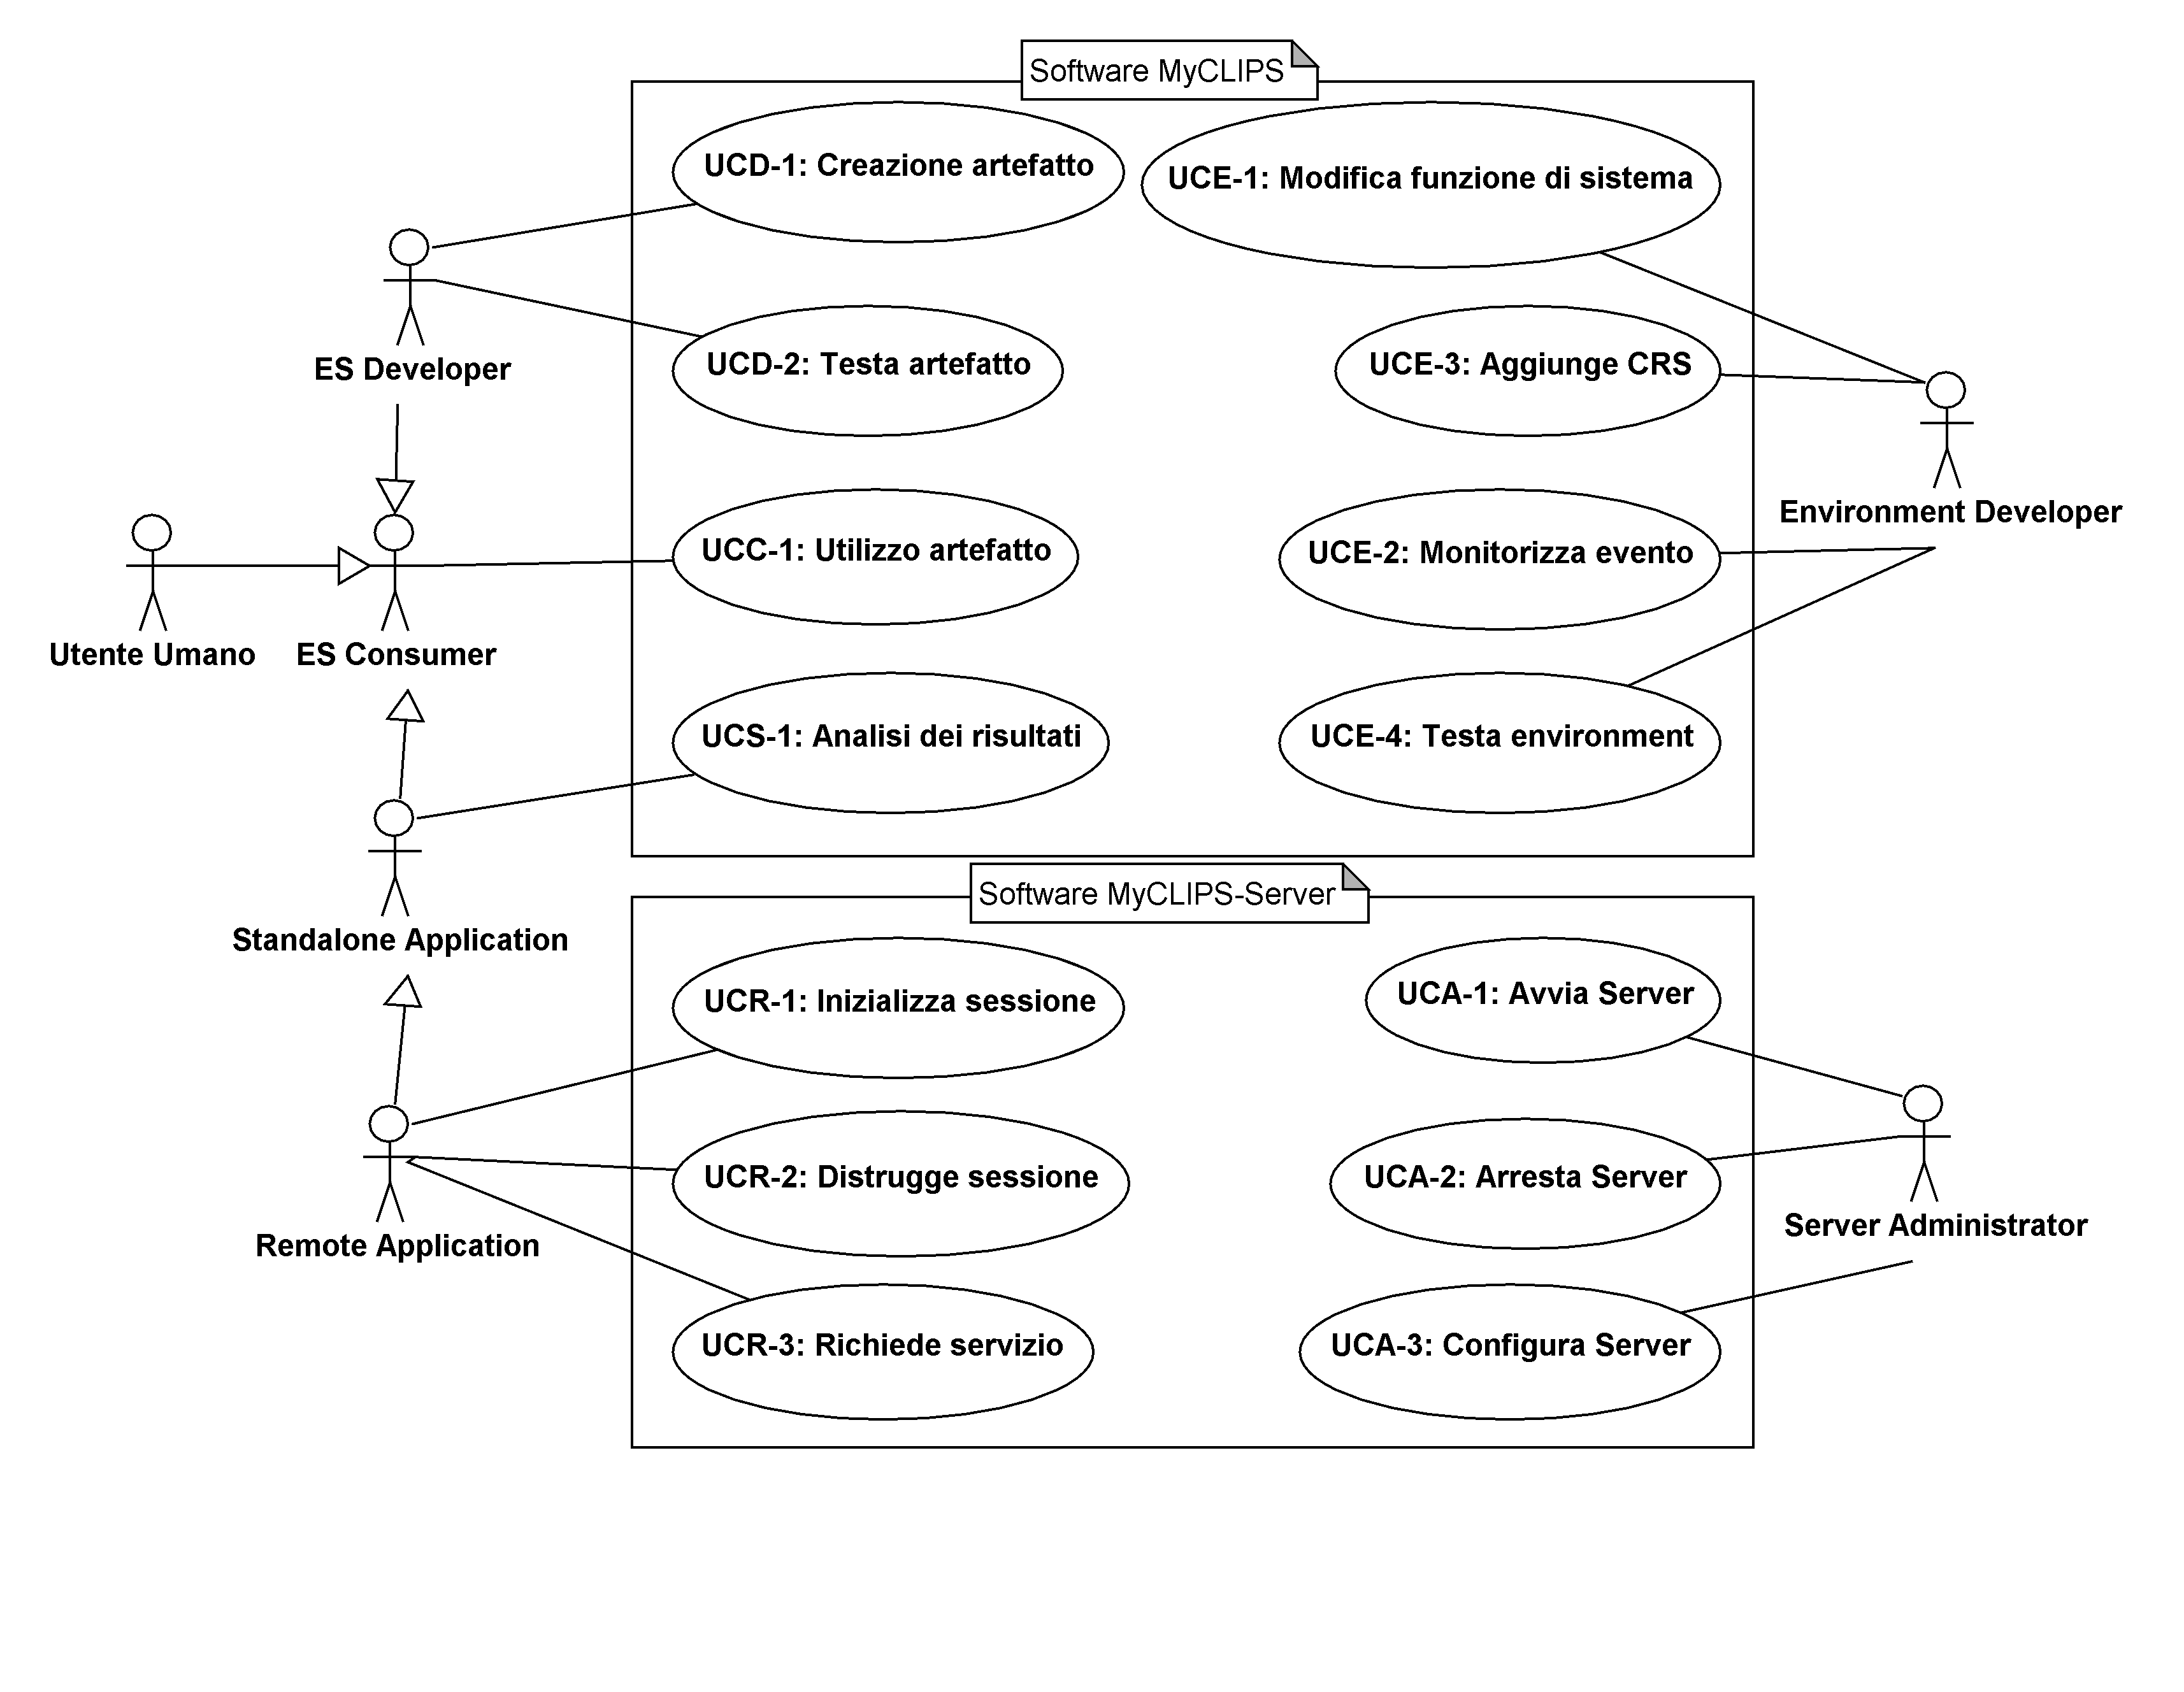
\includegraphics[width=1.2\textwidth, angle=270]{Immagini/Capitolo2/UseCases/Vista-generale.png}
\caption{Vista generale dei casi d'uso principali}\label{fig:uc-vista-generale}
\end{figure}


I casi d'uso vengono organizzati in quattro gruppi differenti (\figurename~\ref{fig:uc-vista-generale}). Il gruppo di appartenenza di ognuno, indicato dal prefisso inserito nel nome, viene associato tenendo conto dell'attore principale al quale \emph{use case} fa riferimento. Il formato del nome di ogni caso d'uso seguirà quindi questa convenzione:
\begin{center}
UC[\emph{Attore}]-[\emph{Sezione}].[\emph{Gruppo}].[\emph{SottoGruppo}]: [\emph{Descrizione breve}]
\end{center}
dove:


\begin{description}
	\item[Attore] indica l'attore principale relazionato con il caso d'uso: \textbf{E} per \emph{Environment Developer}, \textbf{A} per \emph{Server Administrator}, \textbf{S} per \emph{Standalone Application}, \textbf{R} per \emph{Remote Application}, \textbf{D} per \emph{ES Developer} e \textbf{C} per \emph{ES Consumer}. Non è presente nessuno codice per l'attore \emph{Utente umano} in quanto non esiste alcun caso d'uso relativo esclusivamente ad esso.

	\item[Sezione] indica una delle sezioni principali presenti nella vista generale fornita in \figurename~\ref{fig:uc-vista-generale}.
	
	\item[Gruppo] e \textbf{SottoGruppo} esplicitano un'organizzazione gerarchica dei casi d'uso.

\end{description}

\pagebreak

\subsubsection{UCC-1: Utilizzo artefatto}

%UCC-1: Utilizzo artefatto

\begin{figure}
\centering
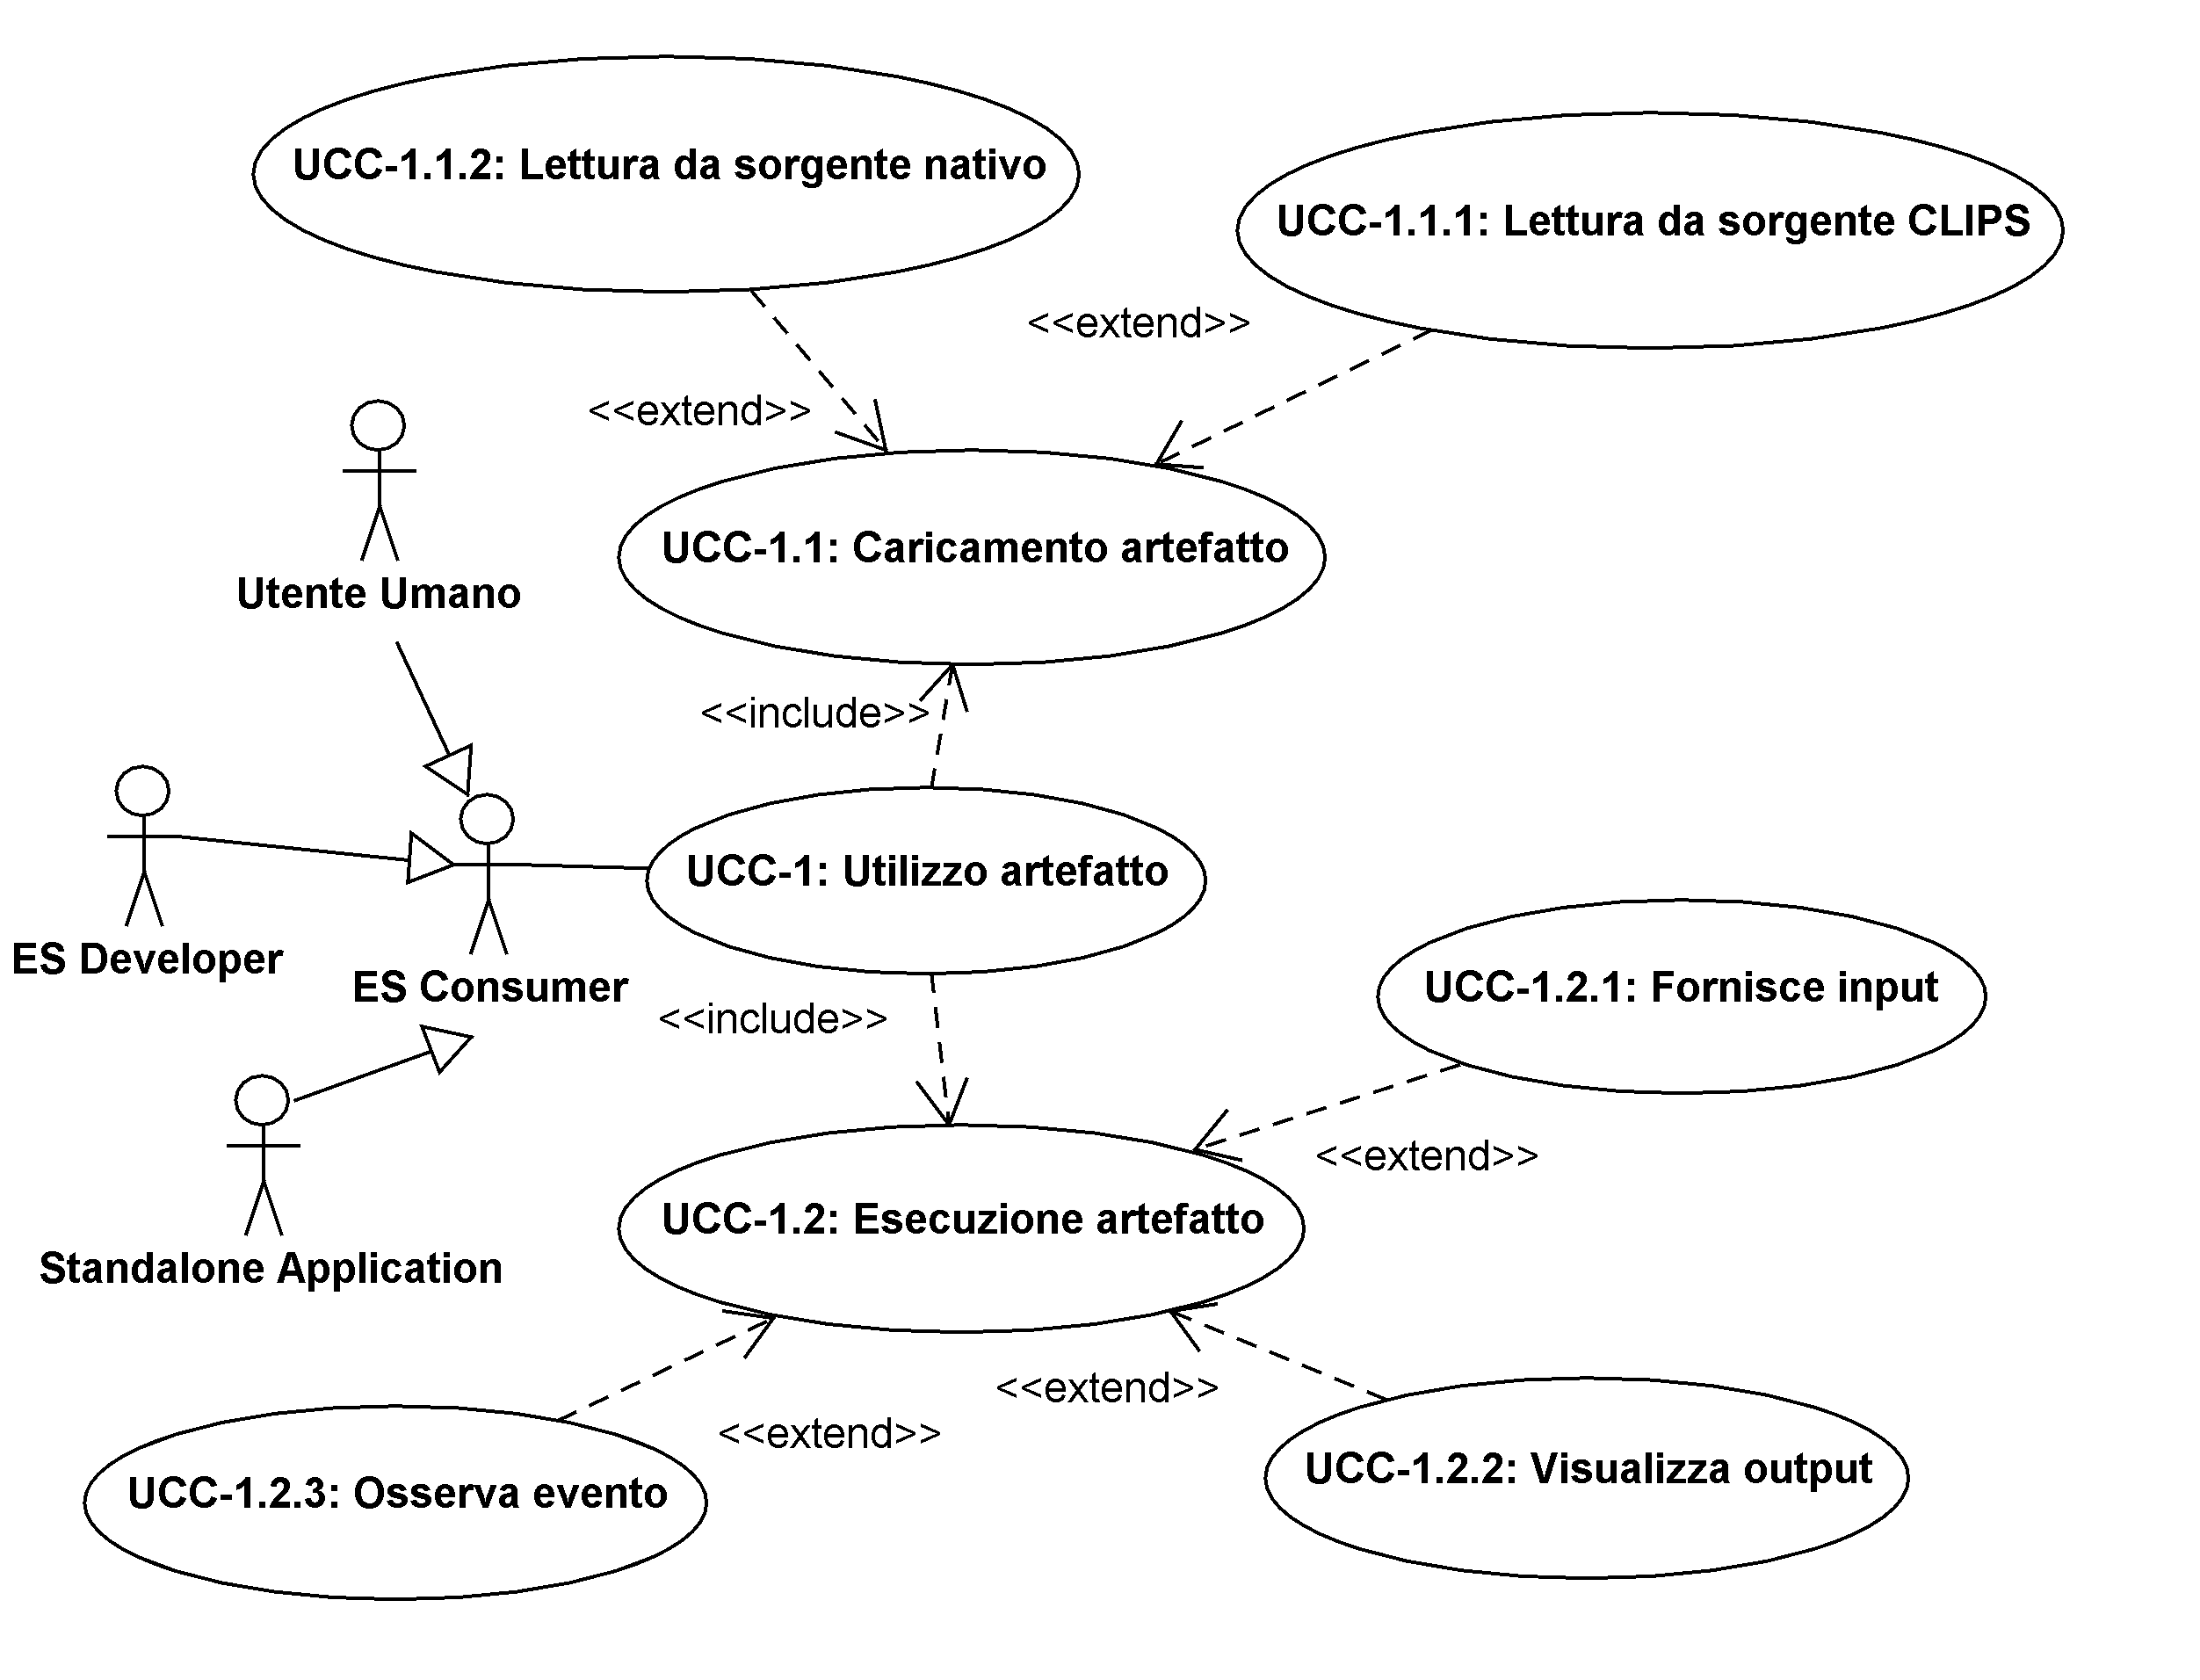
\includegraphics[width=1\textwidth]{Immagini/Capitolo2/UseCases/UCC-1.png}
\caption{Diagramma dei casi d'uso UCC-1}\label{fig:uc-ucc-1}
\end{figure}


\begin{itemize}
	\item \textbf{Attori:} ES Consumer
	\item \textbf{Scopo e descrizione:} un ES Consumer deve poter utilizzare un artefatto precedentemente creato, caricandolo e successivamente eseguendolo.
	\item \textbf{Pre-condizioni:} il software è correttamente configurato nel sistema
	\item \textbf{Post-condizioni:} il software ha eseguito tutte le operazioni desiderate
	\item \textbf{Flusso principale degli eventi:}
		\begin{enumerate}
			\item l'ES Consumer richiede al software di effettuare il caricamento di un artefatto (si veda caso d'uso \emph{UCC-1.1}).
			\item l'ES Consumer richiede al software di eseguire un artefatto (si veda caso d'uso \emph{UCC-1.2}).
		\end{enumerate}
\end{itemize}


\paragraph{UCC-1.1: Caricamento artefatto}

La descrizione comprende quelle dei casi d'uso \emph{UCC-1.1.1} e \emph{UCC-1.1.2} in quanto identici, a meno del formato con il quale l'artefatto viene fornito.

\begin{itemize}
	\item \textbf{Attori:} ES Consumer
	\item \textbf{Scopo e descrizione:} un ES Consumer deve avere la possibilità di caricare nel sistema un artefatto formalizzato in codice sorgente nativo o codice sorgente CLIPS
	\item \textbf{Pre-condizioni:} il software è correttamente configurato nel sistema
	\item \textbf{Post-condizioni:} il software ha eseguito le operazioni di caricamento ed il suo stato rispecchia quello descritto nell'artefatto
	\item \textbf{Flusso principale degli eventi:}
		\begin{enumerate}
			\item l'ES Consumer richiede al software di caricare un artefatto
			\begin{itemize}
				\item l'ES Consumer può fornire un artefatto in formato nativo
				\item l'ES Consumer può fornire un artefatto in formatto CLIPS
			\end{itemize}
			\item Il software analizza l'artefatto
			\item Il software esegue il caricamento dei costrutti contenuti nell'artefatto
		\end{enumerate}
	\item \textbf{Flusso alternativo:}
		\begin{enumerate}
			\setcounter{enumi}{2}
			\item se l'ES Consumer ha fornito un artefatto in formato non valido, il software notifica l'errore fornendo la motivazione e la posizione del problema
		\end{enumerate}
\end{itemize}

\paragraph{UCC-1.2: Esecuzione artefatto}

\begin{itemize}
	\item \textbf{Attori:} ES Consumer
	\item \textbf{Scopo e descrizione:} l'ES Consumer deve poter eseguire un artefatto caricato nel sistema. Se l'interazione lo richiede, l'ES Consumer deve essere in grado di fornire informazioni aggiuntive, osservare l'accadimento di un evento e osservare l'output fornito dal sistema
	\item \textbf{Pre-condizioni:} il software ha correttamente caricato un artefatto ed attende istruzioni.
	\item \textbf{Post-condizioni:} il software ha correttamente eseguito le operazioni previste dall'artefatto.
	\item \textbf{Flusso principale degli eventi:}
		\begin{enumerate}
			\item l'ES Consumer richiede l'esecuzione di un artefatto
			\item il sistema esegue le operazioni previste dall'artefatto (si vedano i casi d'uso \emph{UCC-1.2.1}, \emph{UCC-1.2.3})
			\item il sistema fornisce all'ES Consumer i risultati dell'esecuzione		
		\end{enumerate}
	\item \textbf{Flusso alternativo:} 
		\begin{enumerate}
			\setcounter{enumi}{1}
			\item se un'operazione specificata nell'artefatto genera errori, il sistema notifica l'errore all'ES Consumer fornendo informazioni sulla natura del problema.
			\item il sistema ritorna nello stato iniziale
		\end{enumerate}
\end{itemize}


\subparagraph{UCC-1.2.1: Fornisce input}

\begin{itemize}
	\item \textbf{Attori:} ES Consumer
	\item \textbf{Scopo e descrizione:} l'ES Consumer fornisce informazioni aggiuntive 
	\item \textbf{Pre-condizioni:} il sistema richiede informazioni aggiuntive per completare l'esecuzione di un artefatto
	\item \textbf{Post-condizioni:} il sistema prosegue l'esecuzione
	\item \textbf{Flusso principale degli eventi:}
		\begin{enumerate}
			\item il sistema richiede informazioni aggiuntive
			\item l'ES Consumer fornisce le informazioni nelle forme previste dall'artefatto
			\item il sistema valuta le informazioni fornite
			\item il sistema elabora le informazioni fornite
		\end{enumerate}
	\item \textbf{Flusso alternativo:} 
		\begin{enumerate}
			\setcounter{enumi}{2}
			\item il sistema notifica l'invalidità delle informazioni fornite
			\item il flusso riprende dal punto 1 del flusso principale
		\end{enumerate}
\end{itemize}


\subparagraph{UCC-1.2.2: Visualizza output}

\begin{itemize}
	\item \textbf{Attori:} ES Consumer
	\item \textbf{Scopo e descrizione:} l'ES Consumer deve essere in grado di valutare l'output fornito dal sistema al termine di un'operazione
	\item \textbf{Pre-condizioni:} il sistema è pronto ad esegue un'operazione
	\item \textbf{Post-condizioni:} il sistema è pronto ad eseguire una nuova operazione
	\item \textbf{Flusso principale degli eventi:}
		\begin{enumerate}
			\item il sistema esegue un'operazione
			\item il sistema fornisce una visualizzazione del risultato
			\item l'ES Consumer valuta il risultato
		\end{enumerate}
\end{itemize}


\subparagraph{UCC-1.2.3: Osserva evento}

\begin{itemize}
	\item \textbf{Attori:} ES Consumer
	\item \textbf{Scopo e descrizione:} l'ES Consumer deve essere in grado di ricevere notifica del verificarsi di un evento
	\item \textbf{Pre-condizioni:} il sistema è pronto ad eseguire un'operazione
	\item \textbf{Post-condizioni:} il sistema è pronto ad eseguire un'operazione
	\item \textbf{Flusso principale degli eventi:}
		\begin{enumerate}
			\item l'ES Consumer richiede al sistema di eseguire un'operazione
			\item il sistema esegue un'operazione
			\item il sistema notifica all'ES Consumer il verificarsi di un evento
			\item l'ES Consumer valuta l'evento
		\end{enumerate}
\end{itemize}\pagebreak

\subsubsection{UCD-1: Creazione artefatto}

%UCD-1: Creazione artefatto

\begin{figure}
\centering
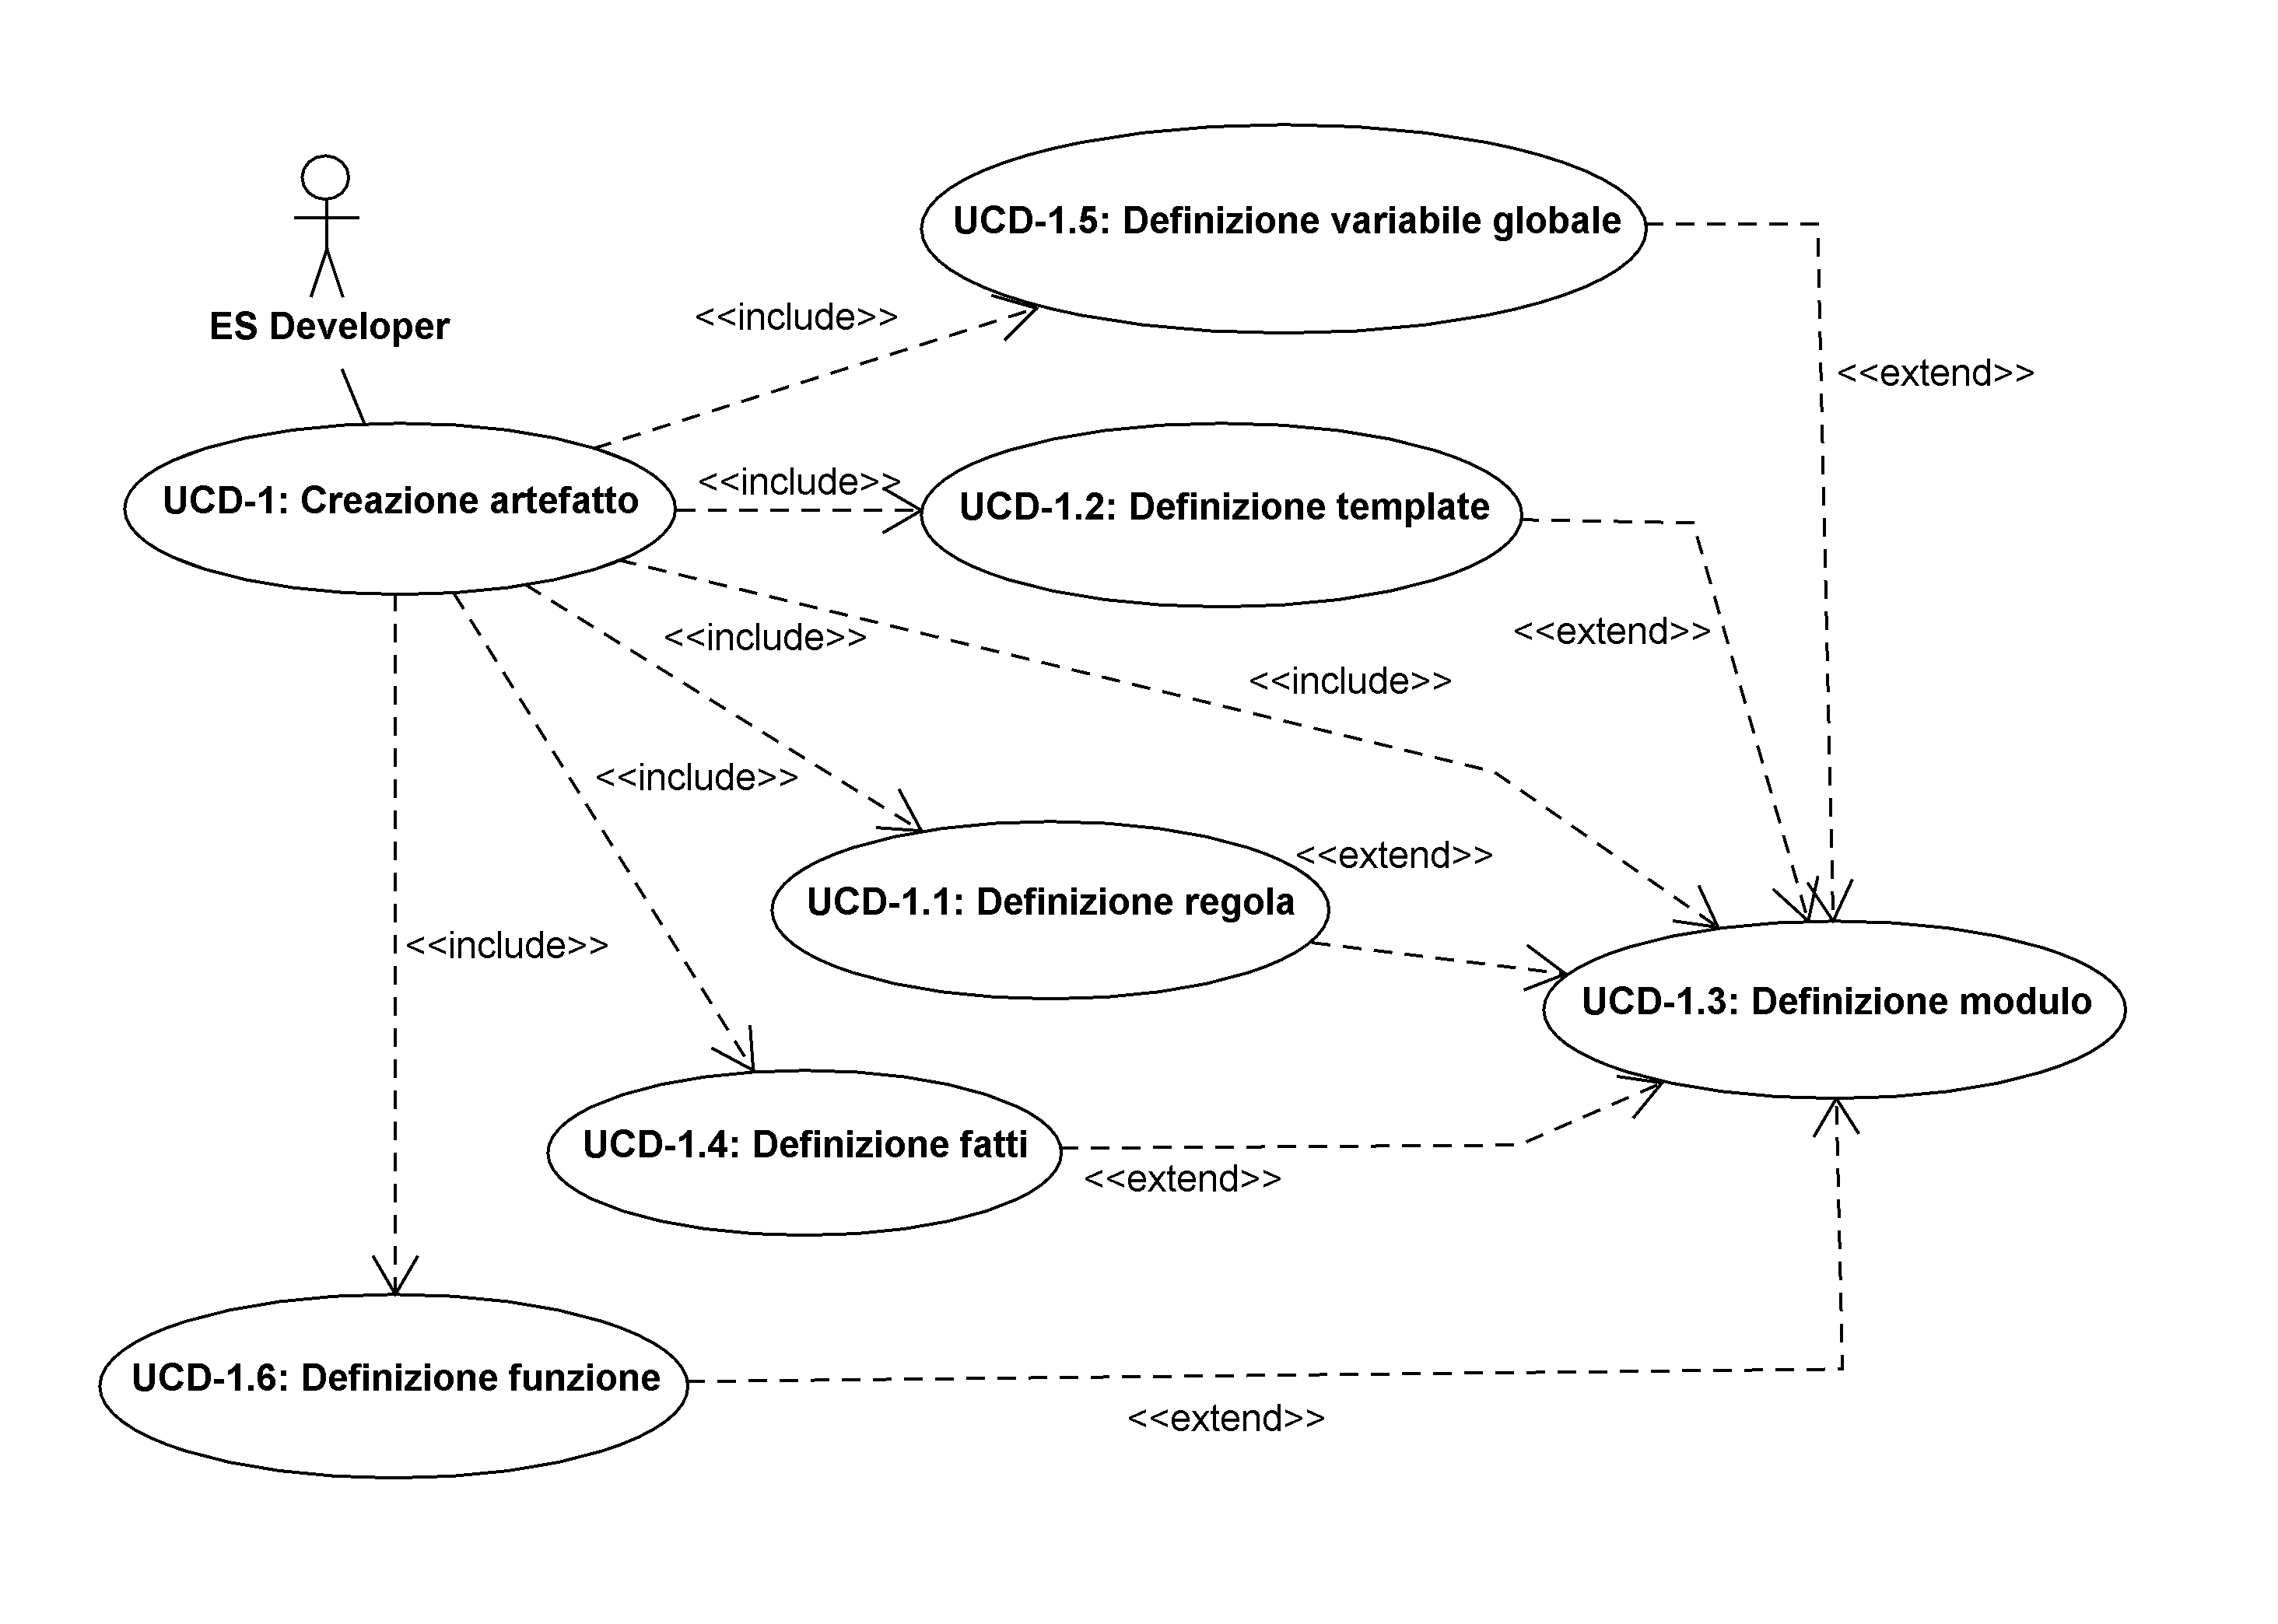
\includegraphics[width=1.1\textwidth]{Immagini/Capitolo2/UseCases/UCD-1.png}
\caption{Diagramma dei casi d'uso UCD-1}\label{fig:uc-ucd-1}
\end{figure}


\begin{itemize}
	\item \textbf{Attori:} ES Developer
	\item \textbf{Scopo e descrizione:} un ES Developer deve essere in grado di definire i costrutti necessari alla realizzazione di un artefatto.
	\item \textbf{Pre-condizioni:} il software fornisce almeno un linguaggio di specifica
	\item \textbf{Post-condizioni:} un artefatto è stato serializzato tramite il linguaggio di specifica
	\item \textbf{Flusso principale degli eventi:}
		\begin{enumerate}
			\item l'ES Developer definisce una serie di costrutti (si vedano i casi d'uso \emph{UCD-1.1}, \emph{UCD-1.2}, \emph{UCD-1.3}, \emph{UCD-1.4}, \emph{UCD-1.5}, \emph{UCD-1.6}).
			\begin{itemize}
				\item l'ES Developer può formalizzarlo in formato nativo
				\item l'ES Developer può formalizzarlo in formatto CLIPS
			\end{itemize}
			\item l'ES Consumer verifica la correttezza dell'artefatto (si veda il caso d'uso \emph{UCD-1.2}).
		\end{enumerate}
\end{itemize}


\paragraph{UCD-1.1: Definizione regola}

\begin{itemize}
	\item \textbf{Attori:} ES Developer
	\item \textbf{Scopo e descrizione:} un ES Developer deve essere in grado di definire una regola tramite un linguaggio di specifica fornito dal sistema.
	\item \textbf{Pre-condizioni:} il software fornisce almeno un linguaggio di specifica
	\item \textbf{Post-condizioni:} la definizione di una regola è stata aggiunta ad un artefatto
	\item \textbf{Flusso principale degli eventi:}
		\begin{enumerate}
			\item l'ES Developer definisce una regola
			\begin{itemize}
				\item l'ES Developer può formalizzarli in formato nativo
				\item l'ES Developer può formalizzarli in formatto CLIPS
			\end{itemize}
		\end{enumerate}
	\item \textbf{Flusso alternativo:}
		\begin{enumerate}
			\item se l'ES Developer ha definito precedentemente un modulo, l'ES Developer può definire una regola come componente del modulo.
		\end{enumerate}
\end{itemize}


\paragraph{UCD-1.2: Definizione template}

\begin{figure}[h]
\centering
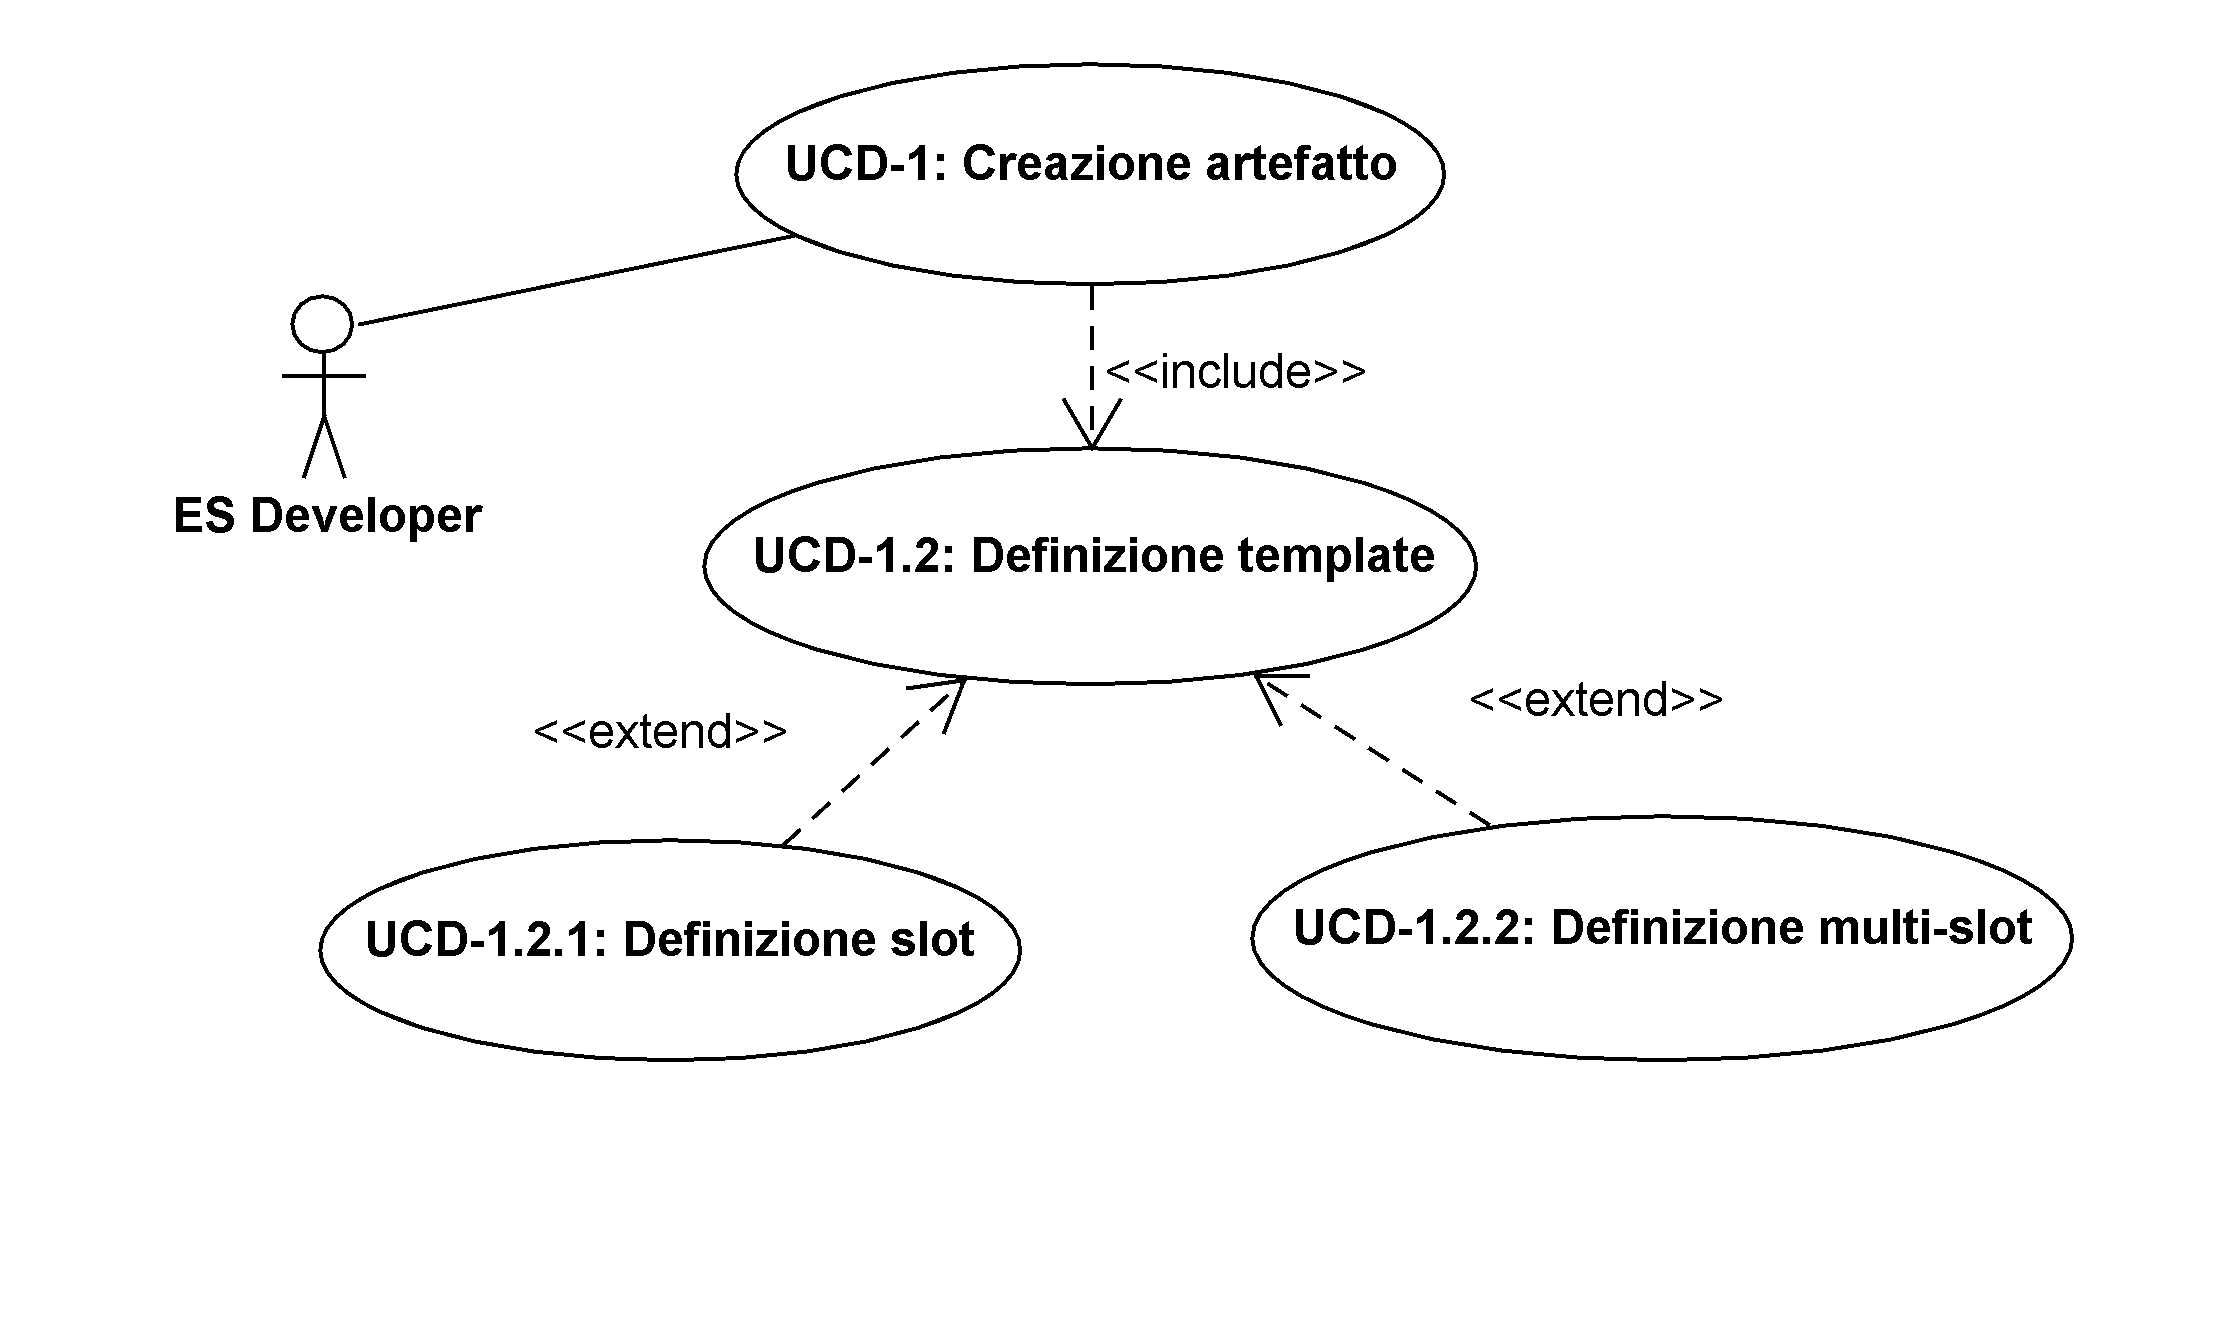
\includegraphics[width=1\textwidth]{Immagini/Capitolo2/UseCases/UCD-1_2.png}
\caption{Diagramma dei casi d'uso UCD-1.2}\label{fig:uc-ucd-1.2}
\end{figure}

\begin{itemize}
	\item \textbf{Attori:} ES Developer
	\item \textbf{Scopo e descrizione:} l'ES Developer deve essere in grado di definire un template di fatti tramite un linguaggio di specifica fornito dal sistema.
	\item \textbf{Pre-condizioni:} il software fornisce almeno un linguaggio di specifica.
	\item \textbf{Post-condizioni:} la definizione di un template di fatti è stato aggiunto ad un artefatto
	\item \textbf{Flusso principale degli eventi:}
		\begin{enumerate}
			\item l'ES Developer definisce un template di fatti
			\item l'ES Developer definisce il formato del template di fatti (si vedano i casi d'uso \emph{UCD-1.2.1}, \emph{UCD-1.2.2})
		\end{enumerate}
	\item \textbf{Flusso alternativo:} 
		\begin{enumerate}
			\item se l'ES Developer ha definito precedentemente un modulo, l'ES Developer può definire un template di fatti come componente di un modulo
		\end{enumerate}
\end{itemize}

\subparagraph{UCD-1.2.1: Definizione slot}

\begin{itemize}
	\item \textbf{Attori:} ES Developer
	\item \textbf{Scopo e descrizione:} l'ES Developer deve essere in grado di definire il formato di uno slot appartenente ad un template di fatti
	\item \textbf{Pre-condizioni:} il software fornisce un linguaggio di specifica, l'ES developer ha definito un template di fatti
	\item \textbf{Post-condizioni:} il formato dello slot è stato aggiunto alla definizione di template di fatti
	\item \textbf{Flusso principale degli eventi:}
		\begin{enumerate}
			\item l'ES Developer definisce un template
			\item l'ES Developer definisce un nuovo slot fornendo il nome (stringa alfanumerica) da attribuire allo stesso
			\begin{enumerate}
				\item l'ES Developer può definire una restrizione di tipo al contenuto dello slot
				\item l'ES Developer può definire un valore di \emph{default} per lo slot
			\end{enumerate}
		\end{enumerate}
	\item \textbf{Flusso alternativo:} 
		\begin{enumerate}
			\setcounter{enumi}{1}
			\item se l'ES Developer ha fornito un nome già usato da un altro slot o multi-slot presente, il sistema rifiuta la definizione notificando un errore.
		\end{enumerate}
\end{itemize}

\subparagraph{UCD-1.2.2: Definizione multi-slot}

\begin{itemize}
	\item \textbf{Attori:} ES Developer
	\item \textbf{Scopo e descrizione:} l'ES Developer deve essere in grado di definire il formato di un multi-slot appartenente ad un template di fatti
	\item \textbf{Pre-condizioni:} il software fornisce un linguaggio di specifica, l'ES Developer ha definito un template di fatti
	\item \textbf{Post-condizioni:} il formato del multi-slot è stato aggiunto alla definizione di template di fatti
	\item \textbf{Flusso principale degli eventi:}
		\begin{enumerate}
			\item l'ES Developer definisce un template
			\item l'ES Developer definisce un nuovo multi-slot fornendo il nome (stringa alfanumerica) da attribuire allo stesso
			\begin{enumerate}
				\item l'ES Developer può definire delle restrizioni di tipo al contenuto dello slot
				\item l'ES Developer può definire dei valori di \emph{default} per il multi-slot
			\end{enumerate}
		\end{enumerate}
	\item \textbf{Flusso alternativo:} 
		\begin{enumerate}
			\setcounter{enumi}{1}
			\item se l'ES Developer ha fornito un nome già usato da un altro slot o multi-slot presente, il sistema rifiuta la definizione notificando un errore.
		\end{enumerate}
\end{itemize}


\paragraph{UCD-1.3: Definizione modulo}

\begin{figure}[h]
\centering
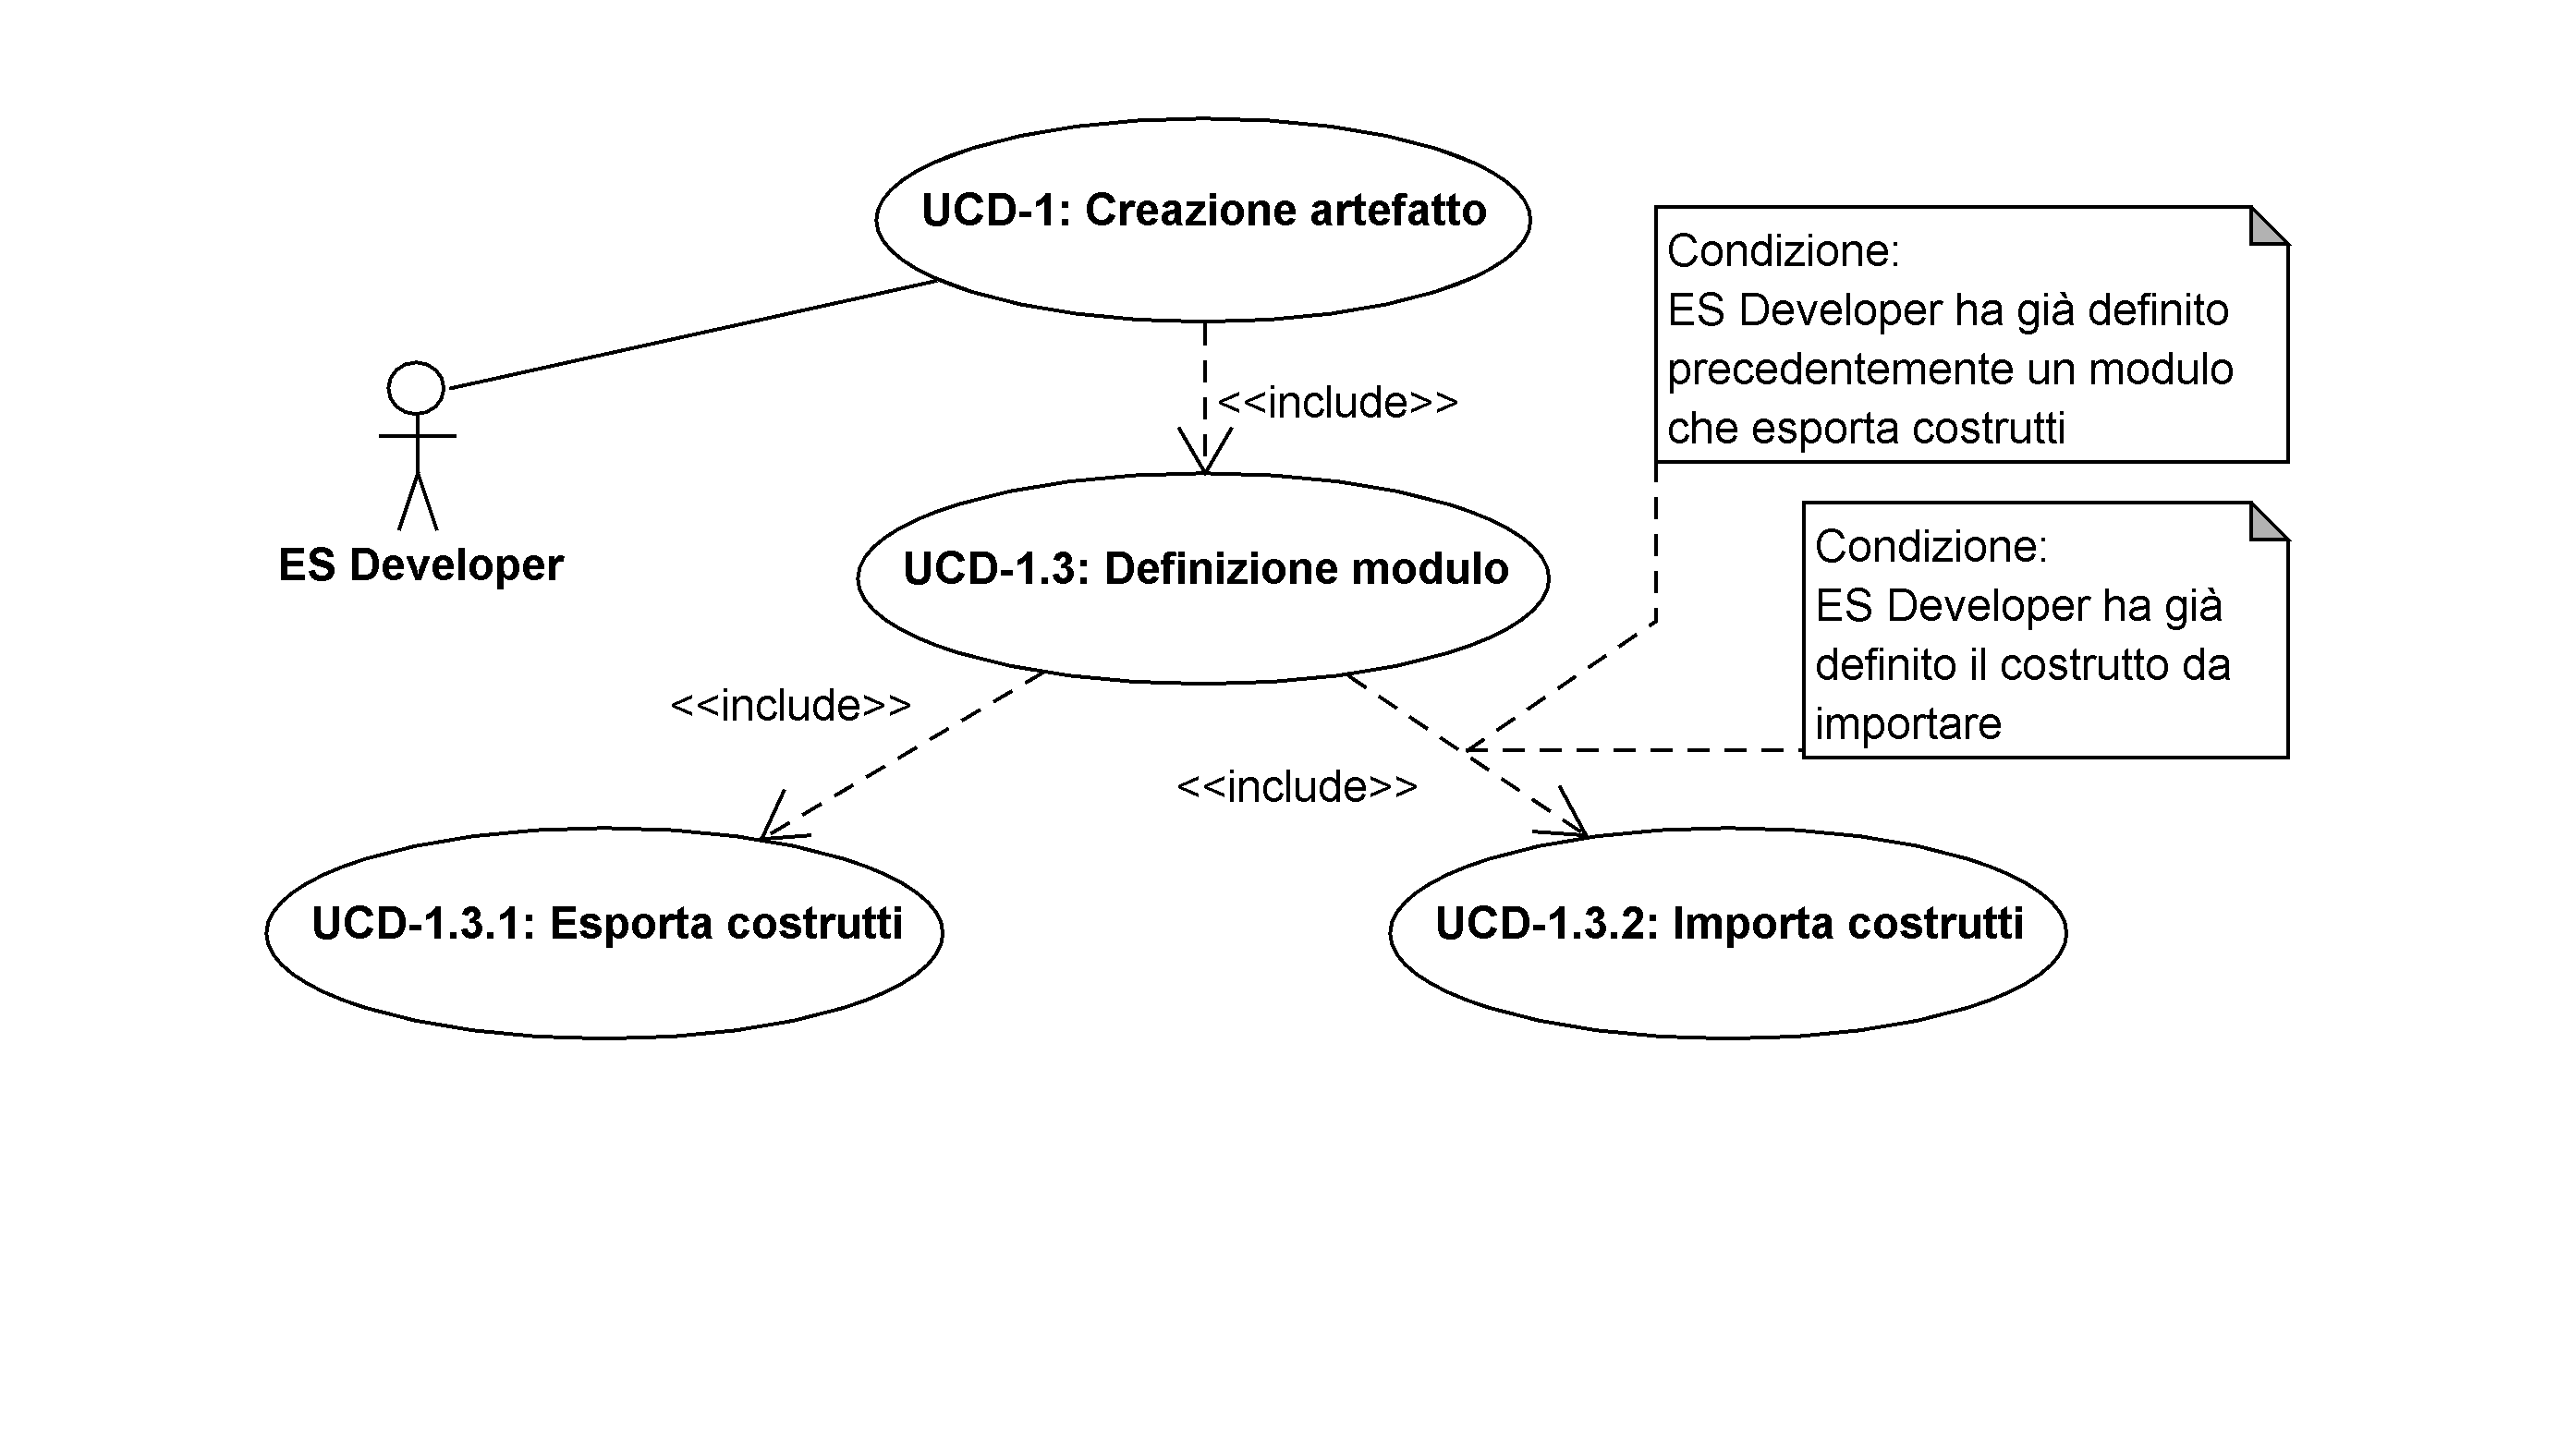
\includegraphics[width=1\textwidth]{Immagini/Capitolo2/UseCases/UCD-1_3.png}
\caption{Diagramma dei casi d'uso UCD-1.3}\label{fig:uc-ucd-1.3}
\end{figure}

\begin{itemize}
	\item \textbf{Attori:} ES Developer
	\item \textbf{Scopo e descrizione:} l'ES Developer deve essere in grado di definire un modulo tramite un linguaggio di specifica fornito dal sistema.
	\item \textbf{Pre-condizioni:} il software fornisce almeno un linguaggio di specifica.
	\item \textbf{Post-condizioni:} la definizione di un modulo è stata aggiunta ad un artefatto.
	\item \textbf{Flusso principale degli eventi:}
		\begin{enumerate}
			\item l'ES Developer definisce un modulo specificandone il nome
			\item l'ES Developer definisce una serie di costrutti da esportare (si veda il caso d'uso \emph{UCD-1.3.1})
			\item l'ES Developer definisce una serie di costrutti da importare da un altro modulo (si veda il caso d'uso \emph{UCD-1.3.2})
		\end{enumerate}
		
	\item \textbf{Flusso alternativo:} 
		\begin{enumerate}
			\setcounter{enumi}{0}
			\item se l'ES Developer fornisce un nome già utilizzato da un altro modulo, il sistema rifiuta la definizione e notifica l'errore.
			\item il sistema ritorna nello stato iniziale.
		\end{enumerate}
		
\end{itemize}

\subparagraph{UCD-1.3.1: Esporta costrutti}

\begin{itemize}
	\item \textbf{Attori:} ES Developer
	\item \textbf{Scopo e descrizione:} l'ES Developer deve essere in grado di specificare l'esportazione di un costrutto relativo al modulo tramite un linguaggio di specifica fornito dal sistema
	\item \textbf{Pre-condizioni:} il sistema fornisce un linguaggio di specifica, l'ES Developer ha definito un modulo
	\item \textbf{Post-condizioni:} il sistema aggiunge il nome del costrutto esportato in un insieme di elementi importabili da altri moduli
	\item \textbf{Flusso principale degli eventi:}
		\begin{enumerate}
			\item l'ES Developer definisce un modulo
			\item l'ES Developer definisce un costrutto appartenente al modulo come esportabile
				\begin{itemize}
					\item l'ES Developer può specificare il nome ed il tipo del costrutto
					\item l'ES Developer può specificare il tipo dei costrutti e un valore speciale per definire l'esportazione di tutti i costrutti del tipo indicato
					\item l'ES Developer può specificare un valore speciale per definire l'esportazione di tutti i costrutti di ogni tipo
					\item l'ES Developer può specificare il tipo ed un valore speciale per definire l'esclusione dei costrutti del tipo specificato dalla lista degli elementi esportati
				\end{itemize}
		\end{enumerate}
\end{itemize}


\subparagraph{UCD-1.3.2: Importa costrutti}

\begin{itemize}
	\item \textbf{Attori:} ES Developer
	\item \textbf{Scopo e descrizione:} l'ES Developer deve essere in grado di specificare l'importazione di un costrutto esportato da un modulo tramite un linguaggio di specifica fornito dal sistema
	\item \textbf{Pre-condizioni:} il sistema fornisce un linguaggio di specifica, l'ES Developer ha definito un modulo che esporta un costrutto, l'ES Developer ha definito un modulo
	\item \textbf{Post-condizioni:} il sistema aggiunge la definizione importata all'insieme di definizione del modulo.
	\item \textbf{Flusso principale degli eventi:}
		\begin{enumerate}
			\item l'ES Developer definisce un modulo
			\item l'ES Developer definisce un costrutto appartenente ad un secondo modulo come importabile.
				\begin{itemize}
					\item l'ES Developer può specificare il modulo, il nome ed il tipo del costrutto da importare
					\item l'ES Developer può specificare il modulo, il tipo ed un valore speciale per definite l'importazione di tutti i costrutti del tipo indicato dal modulo indicato
					\item l'ES Developer può specificare il modulo ed un valore speciale per definire l'importazione di tutti i costrutti dal modulo indicato
					
					\item l'ES Developer può specificare il modulo, il tipo ed un valore speciale per definire l'esclusione di tutti i costrutti del tipo indicato del modulo indicato dall'insieme di costrutti importati
				\end{itemize}
		\end{enumerate}
	\item \textbf{Flusso alternativo \#1:} 
		\begin{enumerate}
			\setcounter{enumi}{1}
			\item se l'ES Developer esegue un'importazione da un modulo non esistente, il sistema rifiuta la definizione e notifica l'errore.
			\item il sistema ritorna nello stato iniziale.
		\end{enumerate}
		
	\item \textbf{Flusso alternativo \#2:} 
		\begin{enumerate}
			\setcounter{enumi}{1}
			\item se l'ES Developer esegue un'importazione di un costrutto non ancora definito da un modulo che lo esporta preventivamente, il sistema rifiuta la definizione e notifica l'errore.
			\item il sistema ritorna nello stato iniziale.
		\end{enumerate}
		
\end{itemize}

\paragraph{UCD-1.4: Definizione fatti} % nome del caso d'uso Gruppo

\begin{figure}
\centering
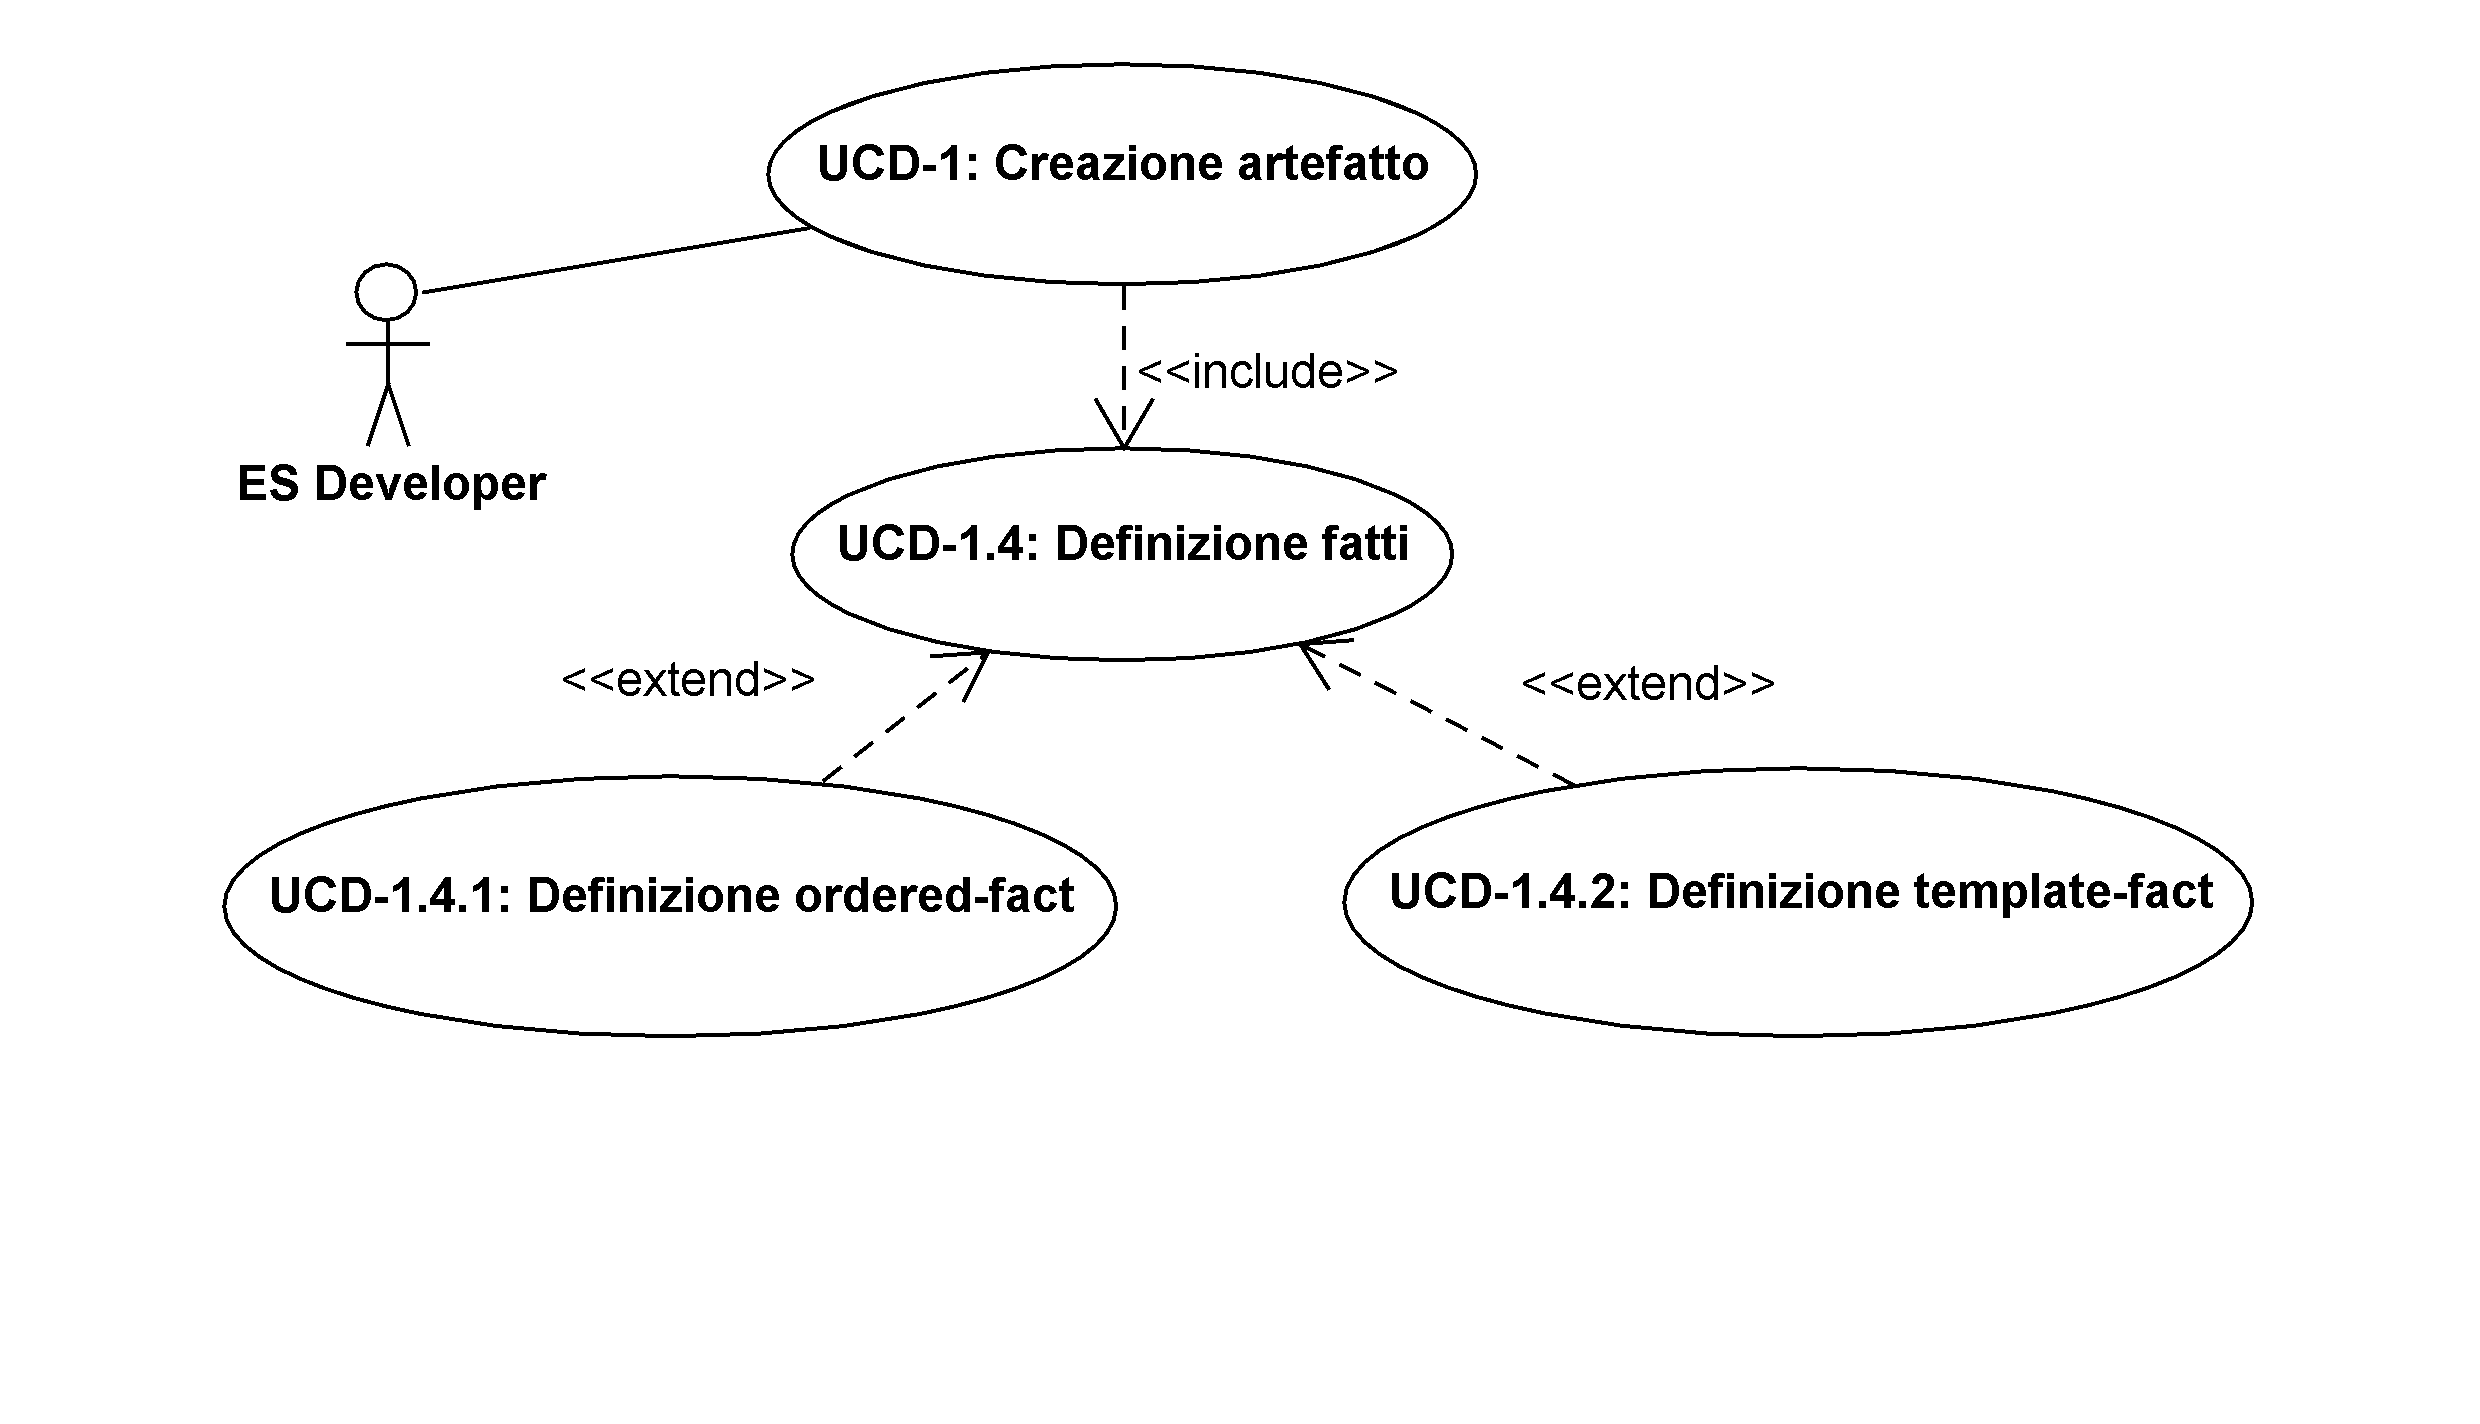
\includegraphics[width=1.1\textwidth]{Immagini/Capitolo2/UseCases/UCD-1_4.png}
\caption{Diagramma dei casi d'uso UCD-1.4}\label{fig:uc-ucd-1.4}
\end{figure}

\begin{itemize}
	\item \textbf{Attori:} ES Developer
	\item \textbf{Scopo e descrizione:} l'ES Developer deve essere in grado di definire un gruppo di fatti iniziali tramite un linguaggio di specifica fornito dal sistema
	\item \textbf{Pre-condizioni:} il software fornisce almeno un linguaggio di specifica
	\item \textbf{Post-condizioni:} la definizione del gruppo di fatti è stata aggiunta ad un artefatto
	\item \textbf{Flusso principale degli eventi:}
		\begin{enumerate}
			\item l'ES Developer definisce un gruppo di fatti specificando il nome
			\item l'ES Developer definisce una serie di fatti da associare al gruppo (si vedano i casi d'uso \emph{UCD-1.4.1} e \emph{UCD-1.4.2})
		\end{enumerate}
	\item \textbf{Flusso alternativo:}
		\begin{enumerate}
			\item se l'ES Developer ha definito precedentemente un modulo, l'ES Developer può definire il gruppo di fatti come componente del modulo.
			\item lo scenario prosegue dal punto 2 del flusso principale
		\end{enumerate}
\end{itemize}

\subparagraph{UCD-1.4.1: Definizione ordered-fact} % nome del caso d'uso SottoGruppo

\begin{itemize}
	\item \textbf{Attori:} ES Developer
	\item \textbf{Scopo e descrizione:}  l'ES Developer deve essere in grado di definire un fatto in notazione \emph{ordered-fact} tramite un linguaggio di specifica fornito dal sistema
	\item \textbf{Pre-condizioni:} il software fornisce almeno un linguaggio di specifica, l'ES Developer ha definito un gruppo di fatti iniziali
	\item \textbf{Post-condizioni:} il fatto in notazione \emph{ordered-fact} è aggiunto al gruppo di fatti iniziali
	\item \textbf{Flusso principale degli eventi:}
		\begin{enumerate}
			\item l'ES Developer definisce un gruppo di fatti iniziali
			\item l'ES Developer definisce un fatto in notazione \emph{ordered-fact} specificando l'elenco di componenti in sequenza
				\begin{itemize}
					\item l'ES Developer può specificare una sequenza di componenti di lunghezza arbitraria
					\item l'ES Developer può specificare una sequenza di componenti di tipo non omogeneo
				\end{itemize}
		\end{enumerate}
	\item \textbf{Flusso alternativo:}
		\begin{enumerate}
			\setcounter{enumi}{1}
			\item l'ES Developer definisce un fatto in notazione \emph{ordered-fact} con componenti identiche a quelle di un fatto specificato in precedenza
			\item il sistema ignora la definizione
		\end{enumerate}
\end{itemize}


\subparagraph{UCD-1.4.2: Definizione template-fact} % nome del caso d'uso SottoGruppo

\begin{itemize}
	\item \textbf{Attori:} ES Developer
	\item \textbf{Scopo e descrizione:}  l'ES Developer deve essere in grado di definire un fatto in notazione \emph{template-fact} tramite un linguaggio di specifica fornito dal sistema
	\item \textbf{Pre-condizioni:} il software fornisce almeno un linguaggio di specifica, l'ES Developer ha definito un gruppo di fatti iniziali
	\item \textbf{Post-condizioni:} il fatto in notazione \emph{template-fact} è aggiunto al gruppo di fatti iniziali
	\item \textbf{Flusso principale degli eventi:}
		\begin{enumerate}
			\item l'ES Developer definisce un gruppo di fatti iniziali
			\item l'ES Developer definisce un fatto in notazione \emph{template-fact} specificando il nome del \emph{template} di riferimento
			\item l'ES Developer definisce i valori degli slot (risp. multi-slot)
				\begin{itemize}
					\item l'ES Developer può specificare una sequenza di componenti di lunghezza arbitraria per i \emph{multi-slot}
					\item l'ES Developer può specificare un elemento per gli \emph{slot}
				\end{itemize}
			\item il sistema completa la definizione del fatto associando i valori di default agli \emph{slot} (risp. \emph{multi-slot}) non definiti.
		\end{enumerate}
	\item \textbf{Flusso alternativo \#1:}
		\begin{enumerate}
			\setcounter{enumi}{1}
			\item l'ES Developer fornisce un nome di template non valido
			\item il sistema rifiuta la definizione e notifica l'errore
			\item il sistema torna allo stato iniziale
		\end{enumerate}
	\item \textbf{Flusso alternativo \#2:}
		\begin{enumerate}
			\setcounter{enumi}{2}
			\item l'ES Developer assegna un valore ad uno \emph{slot} (risp. \emph{multi-slot}) non definito nella definizione del \emph{template}.
			\item il sistema rifiuta la definizione e notifica l'errore
			\item il sistema torna allo stato iniziale
		\end{enumerate}
\end{itemize}


\paragraph{UCD-1.5: Definizione variabile globale} % nome del caso d'uso Gruppo

\begin{itemize}
	\item \textbf{Attori:} ES Developer
	\item \textbf{Scopo e descrizione:}  l'ES Developer deve essere in grado di definire una variabile globale tramite un linguaggio di specifica.
	\item \textbf{Pre-condizioni:} il software fornisce almeno un linguaggio di specifica
	\item \textbf{Post-condizioni:} la definizione della variabile globale è stata aggiunta ad un artefatto
	\item \textbf{Flusso principale degli eventi:}
		\begin{enumerate}
			\item l'ES Developer definisce una variabile globale, indicando nome e valore iniziale
			\item il sistema valuta la definizione
		\end{enumerate}
	\item \textbf{Flusso alternativo \#1:} 
		\begin{enumerate}
			\setcounter{enumi}{1}
			\item se l'ES Developer ha indicato come nome per la variabile globale uno già utilizzato, il valore iniziale fornito viene sostituito a quello della definizione precedente
			\item lo scenario prosegue dal punto 2 del flusso principale
		\end{enumerate}
	\item \textbf{Flusso alternativo \#2:} 
		\begin{enumerate}
			\item se l'ES Developer ha definito precedentemente un modulo, l'ES Developer può definire la variabile globale come componente del modulo.
			\item lo scenario prosegue dal punto 2 del flusso principale
		\end{enumerate}
\end{itemize}

\paragraph{UCD-1.6: Definizione funzione} % nome del caso d'uso Gruppo

\begin{itemize}
	\item \textbf{Attori:} ES Developer
	\item \textbf{Scopo e descrizione:} l'ES Developer deve essere in grado di definire una funzione tramite un linguaggio di specifica
	\item \textbf{Pre-condizioni:} il software fornisce almeno un linguaggio di specifica
	\item \textbf{Post-condizioni:} la definizione della funzione è stata aggiunta ad un artefatto
	\item \textbf{Flusso principale degli eventi:}
		\begin{enumerate}
			\item l'ES Developer definisce una funzione utente, indicando nome, parametri e corpo della funzione
			\item il sistema valuta il nome della funzione
		\end{enumerate}
	\item \textbf{Flusso alternativo \#1:}
		\begin{enumerate}
			\setcounter{enumi}{1}
			\item se il nome fornito dall'ES Developer è già utilizzato da una definizione di funzione (di sistema o utente), il sistema rifiuta la definizione e notifica l'errore
			\item il sistema ritorna allo stato iniziale
		\end{enumerate}
	\item \textbf{Flusso alternativo \#2:}
		\begin{enumerate}
			\item se l'ES Developer ha definito precedentemente un modulo, l'ES Developer può definire la funzione utente come componente del modulo
			\item lo scenario procede dal punto 2 del flusso principale
		\end{enumerate}
\end{itemize}

\pagebreak

\subsubsection{UCD-2: Testa artefatto}

%%UCD-2: Testa artefatto

\begin{figure}
\centering
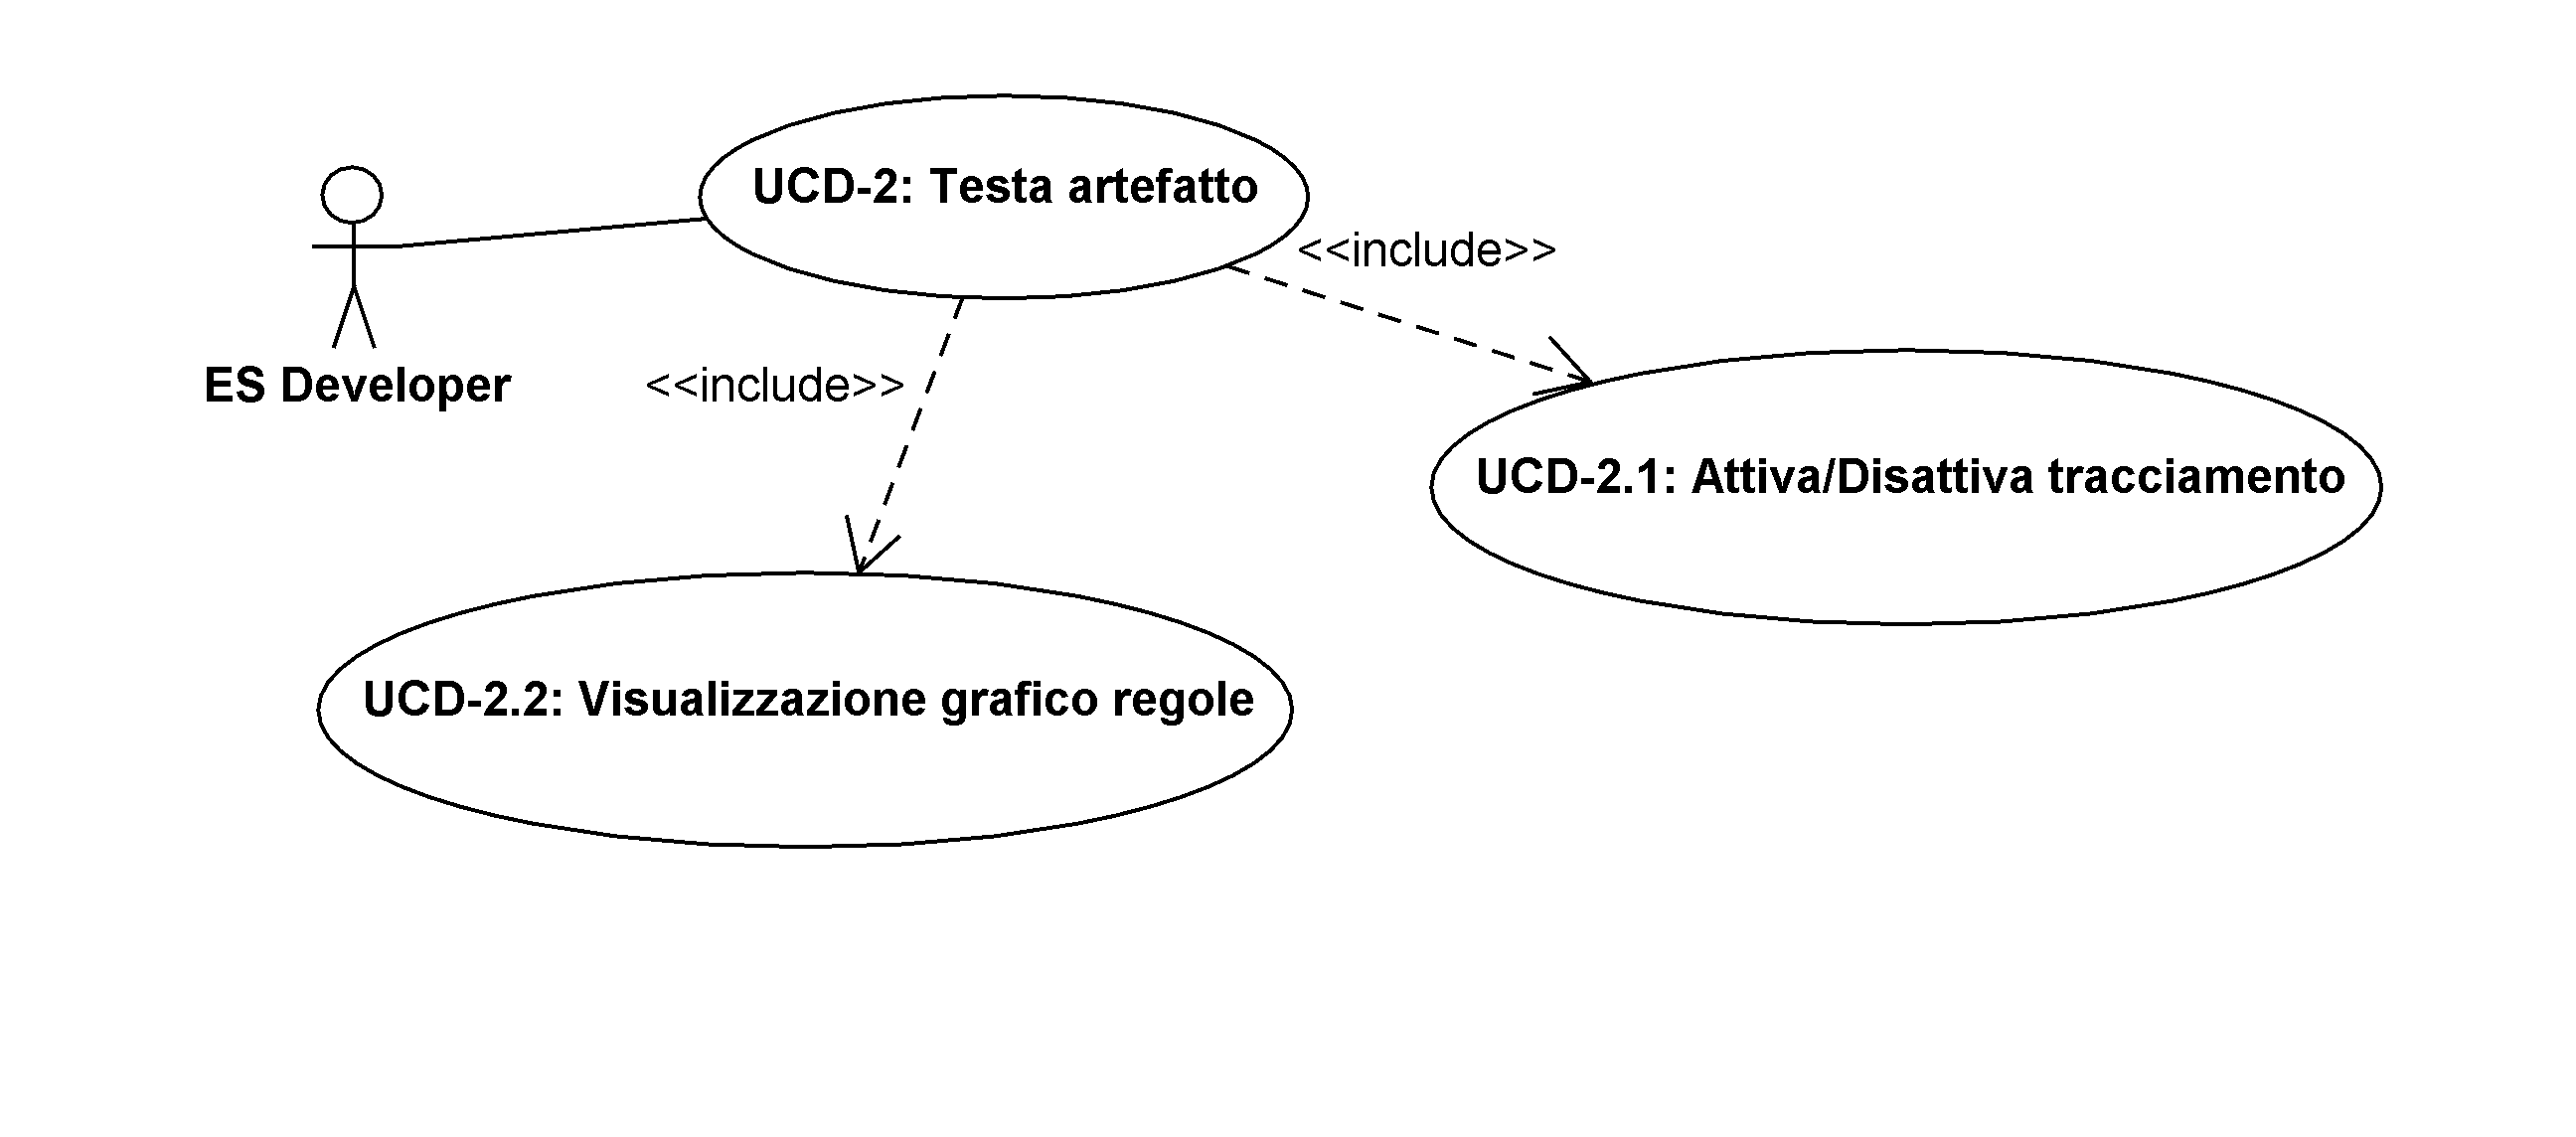
\includegraphics[width=1.1\textwidth]{Immagini/Capitolo2/UseCases/UCD-2.png}
\caption{Diagramma dei casi d'uso UCD-2}\label{fig:uc-ucd-2}
\end{figure}


\begin{itemize}
	\item \textbf{Attori:} ES Developer
	\item \textbf{Scopo e descrizione:} un ES Developer deve essere in grado di testare l'artefatto prodotto valutando un registro del funzionamento dello stesso e le modalità con le quali le definizioni appartenenti all'artefatto vengono interpretate.
	\item \textbf{Pre-condizioni:} l'ES Developer ha realizzato un artefatto, l'artefatto è stato caricato nel sistema. Il sistema attende istruzioni
	\item \textbf{Post-condizioni:} il funzionamento dell'artefatto è stato valutato
	\item \textbf{Flusso principale degli eventi:}
		\begin{enumerate}
			\item l'ES Developer richiede al sistema informazioni per valutare l'artefatto.
			\begin{itemize}
				\item l'ES Developer può richiedere informazioni sull'attività del sistema (si veda caso d'uso \emph{UCD-2.1})
				\item l'ES Developer può richiedere informazioni su come l'artefatto viene interpretato (si veda caso d'uso \emph{UCD-2.2}).
			\end{itemize}
			\item il sistema fornisce le informazioni richieste.
		\end{enumerate}
\end{itemize}


\paragraph{UCD-2.1: Attiva/Disattiva tracciamento}

\begin{figure}
\centering
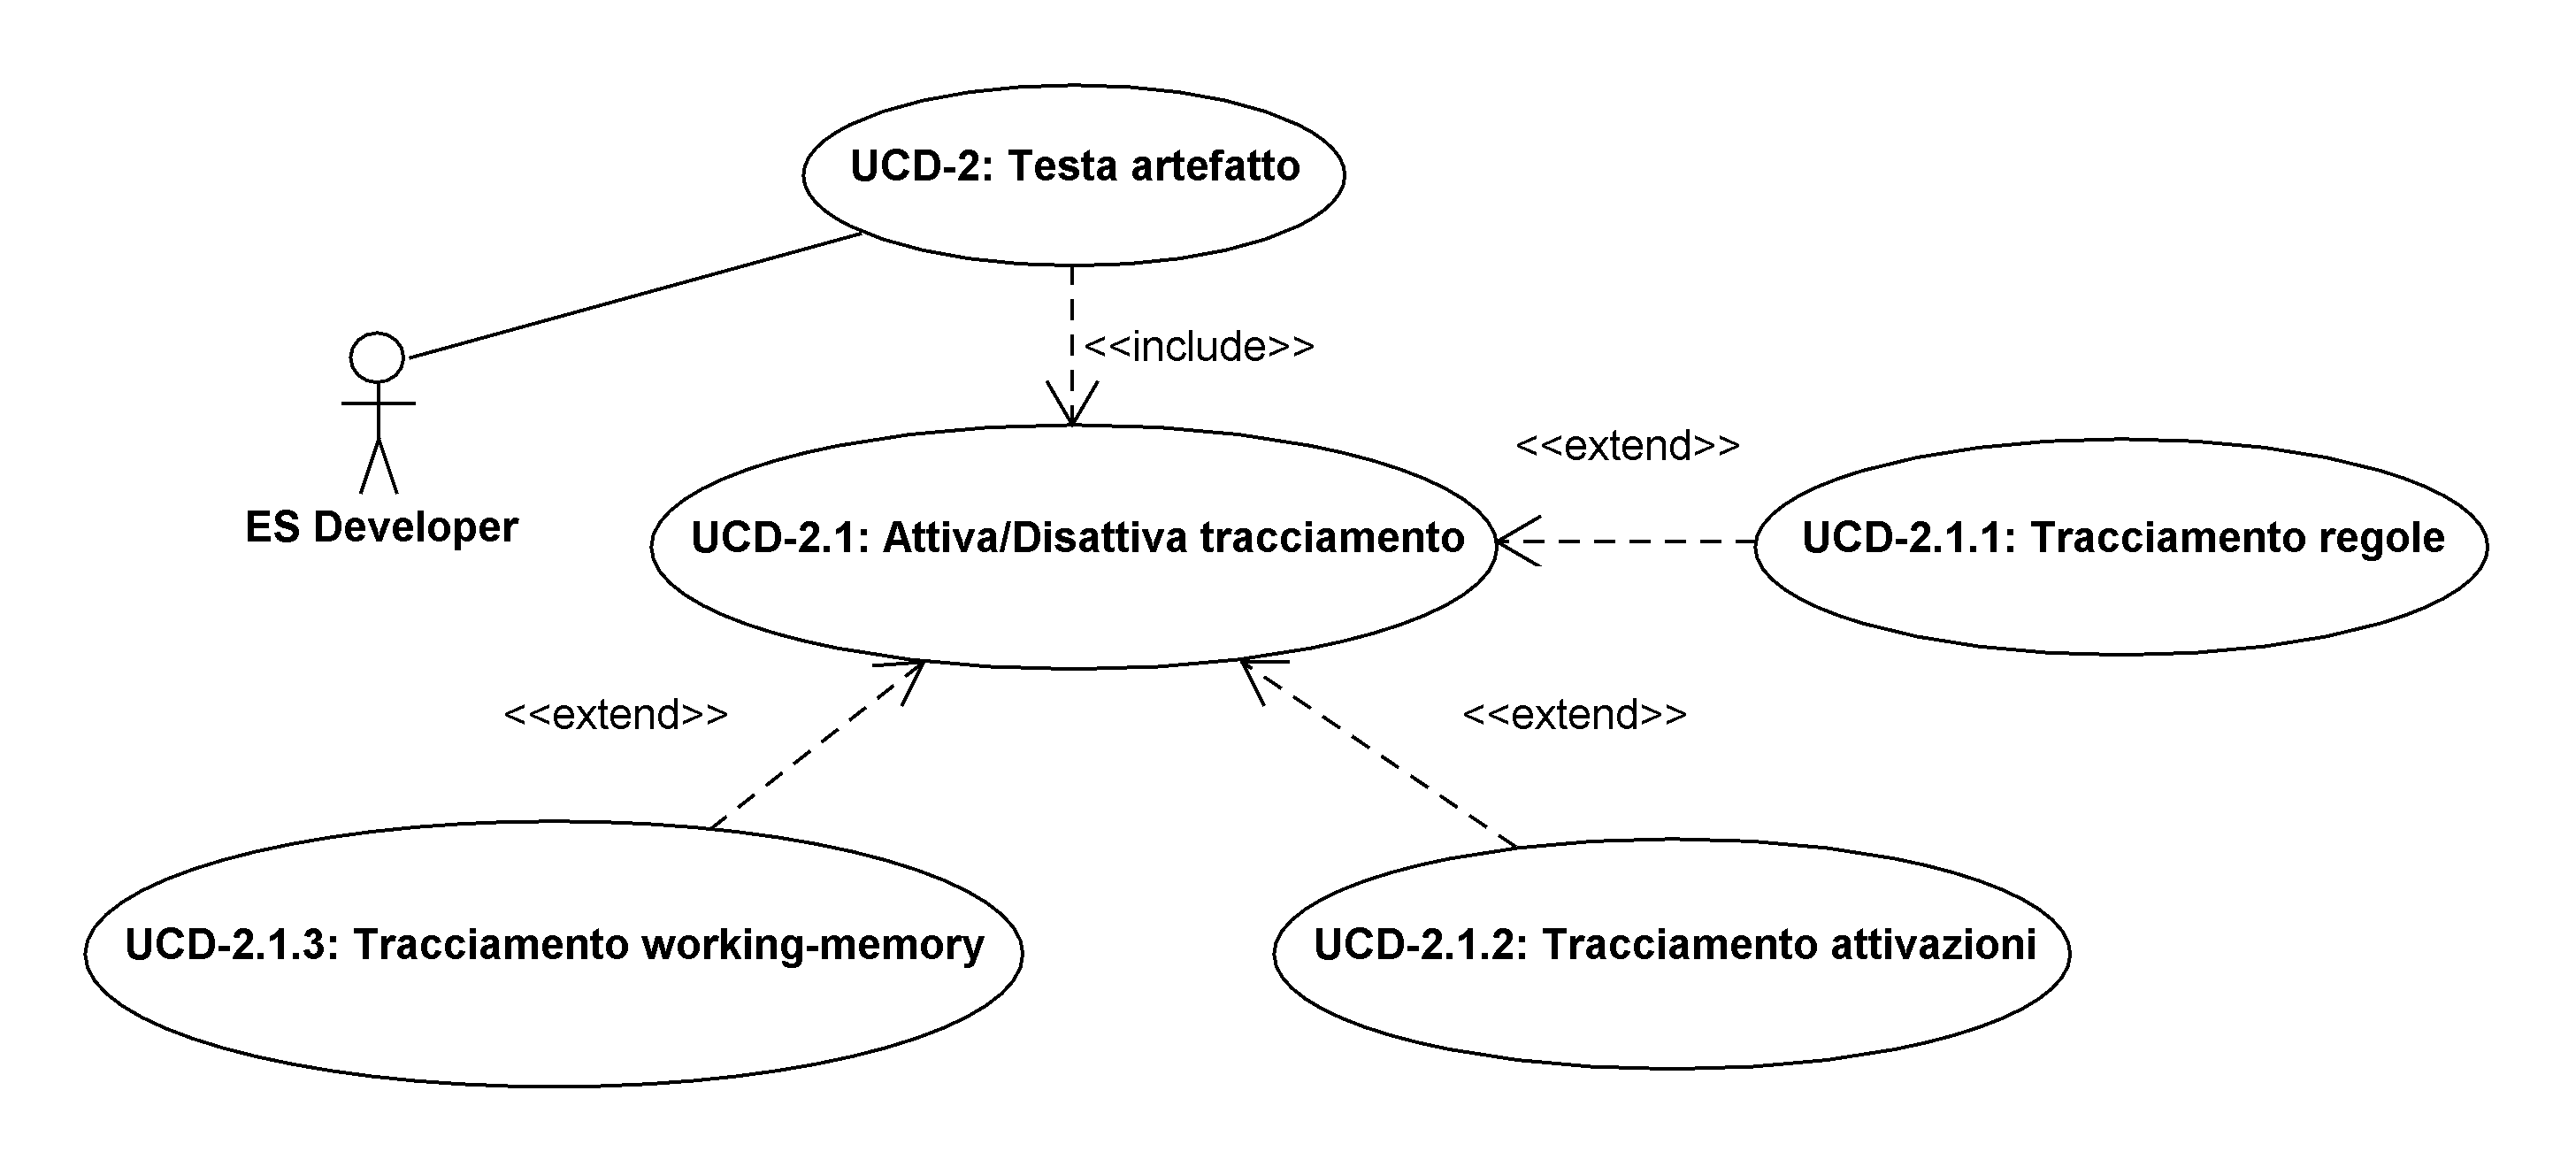
\includegraphics[width=1.1\textwidth]{Immagini/Capitolo2/UseCases/UCD-2_1.png}
\caption{Diagramma dei casi d'uso UCD-2.1}\label{fig:uc-ucd-2.1}
\end{figure}

La descrizione comprende quella dei casi d'uso \emph{UCD-2.1.1}, \emph{UCD-2.1.2}, \emph{UCD-2.1.3} in quanto identici, a meno del tipo di informazioni che vengono tracciate.

\begin{itemize}
	\item \textbf{Attori:} ES Developer
	\item \textbf{Scopo e descrizione:} un ES Developer deve essere in grado di modificare le impostazioni riguardo al tracciamento di regole, attivazioni e modifiche alla \emph{working-memory}.
	\item \textbf{Pre-condizioni:} ES Developer ha caricato un artefatto nel sistema. Il sistema attende istruzioni
	\item \textbf{Post-condizioni:} le impostazioni di tracciamento risultano modificate
	\item \textbf{Flusso principale degli eventi:}
		\begin{enumerate}
			\item l'ES Developer modifica le impostazioni riguardanti il tracciamento
			\begin{itemize}
				\item l'ES Developer può attivare (risp. disattivare) il tracciamento delle regole eseguite
				\item l'ES Developer può attivare (risp. disattivare) il tracciamento delle attivazioni disponibili
				\item l'ES Developer può attivare (risp. disattivare) il tracciamento delle modifiche alla \emph{working-memory}				
			\end{itemize}
			\item il sistema modifica le impostazioni di tracciamento dell'elemento indicato
		\end{enumerate}
	\item \textbf{Flusso alternativo:}
		\begin{enumerate}
			\item l'ES Developer richiede l'attivazione (risp. disattivazione) di un tracciamento già attivo (risp. non attivo).
			\item il sistema ignora la richiesta
		\end{enumerate}
\end{itemize}


\paragraph{UCD-2.2: Visualizzazione grafico regole}

\begin{itemize}
	\item \textbf{Attori:} ES Developer
	\item \textbf{Scopo e descrizione:} un ES Developer deve essere in grado di richiedere informazioni riguardanti le modalità con le quali il sistema interpreta una regola.
	\item \textbf{Pre-condizioni:} ES Developer ha caricato un artefatto nel sistema. Il sistema attende istruzioni
	\item \textbf{Post-condizioni:} Il sistema attende istruzioni
	\item \textbf{Flusso principale degli eventi:}
		\begin{enumerate}
			\item l'ES Developer richiede informazioni riguardanti l'interpretazione di una regola
			\begin{itemize}
				\item l'ES Developer può indicare una regola specificandone il nome
				\item l'ES Developer può indicare un insieme di regole specificandone i nomi
			\end{itemize}
			\item il sistema fornisce le informazioni richieste
		\end{enumerate}
	\item \textbf{Flusso alternativo \#1:}
		\begin{enumerate}
			\item l'ES Developer specifica un nome di regola non valido
			\item il sistema ignora la richiesta, notificando l'errore
		\end{enumerate}
	\item \textbf{Flusso alternativo \#2:}
		\begin{enumerate}
			\item l'ES Developer inserisce un nome non valido specificando un insieme di regole
			\item il sistema ignora la richiesta, notificando l'errore
		\end{enumerate}
\end{itemize}

\pagebreak

\subsubsection{UCE-1: Modifica funzioni di sistema}

%%UCE-1: Modifica funzioni di sistema

Nel proseguo dei paragrafi relativi ai casi d'uso \emph{UCE}, il nome dell'attore \emph{Environment Developer} verrà abbreviato con la sigla \emph{ED}.

\begin{figure}
\centering
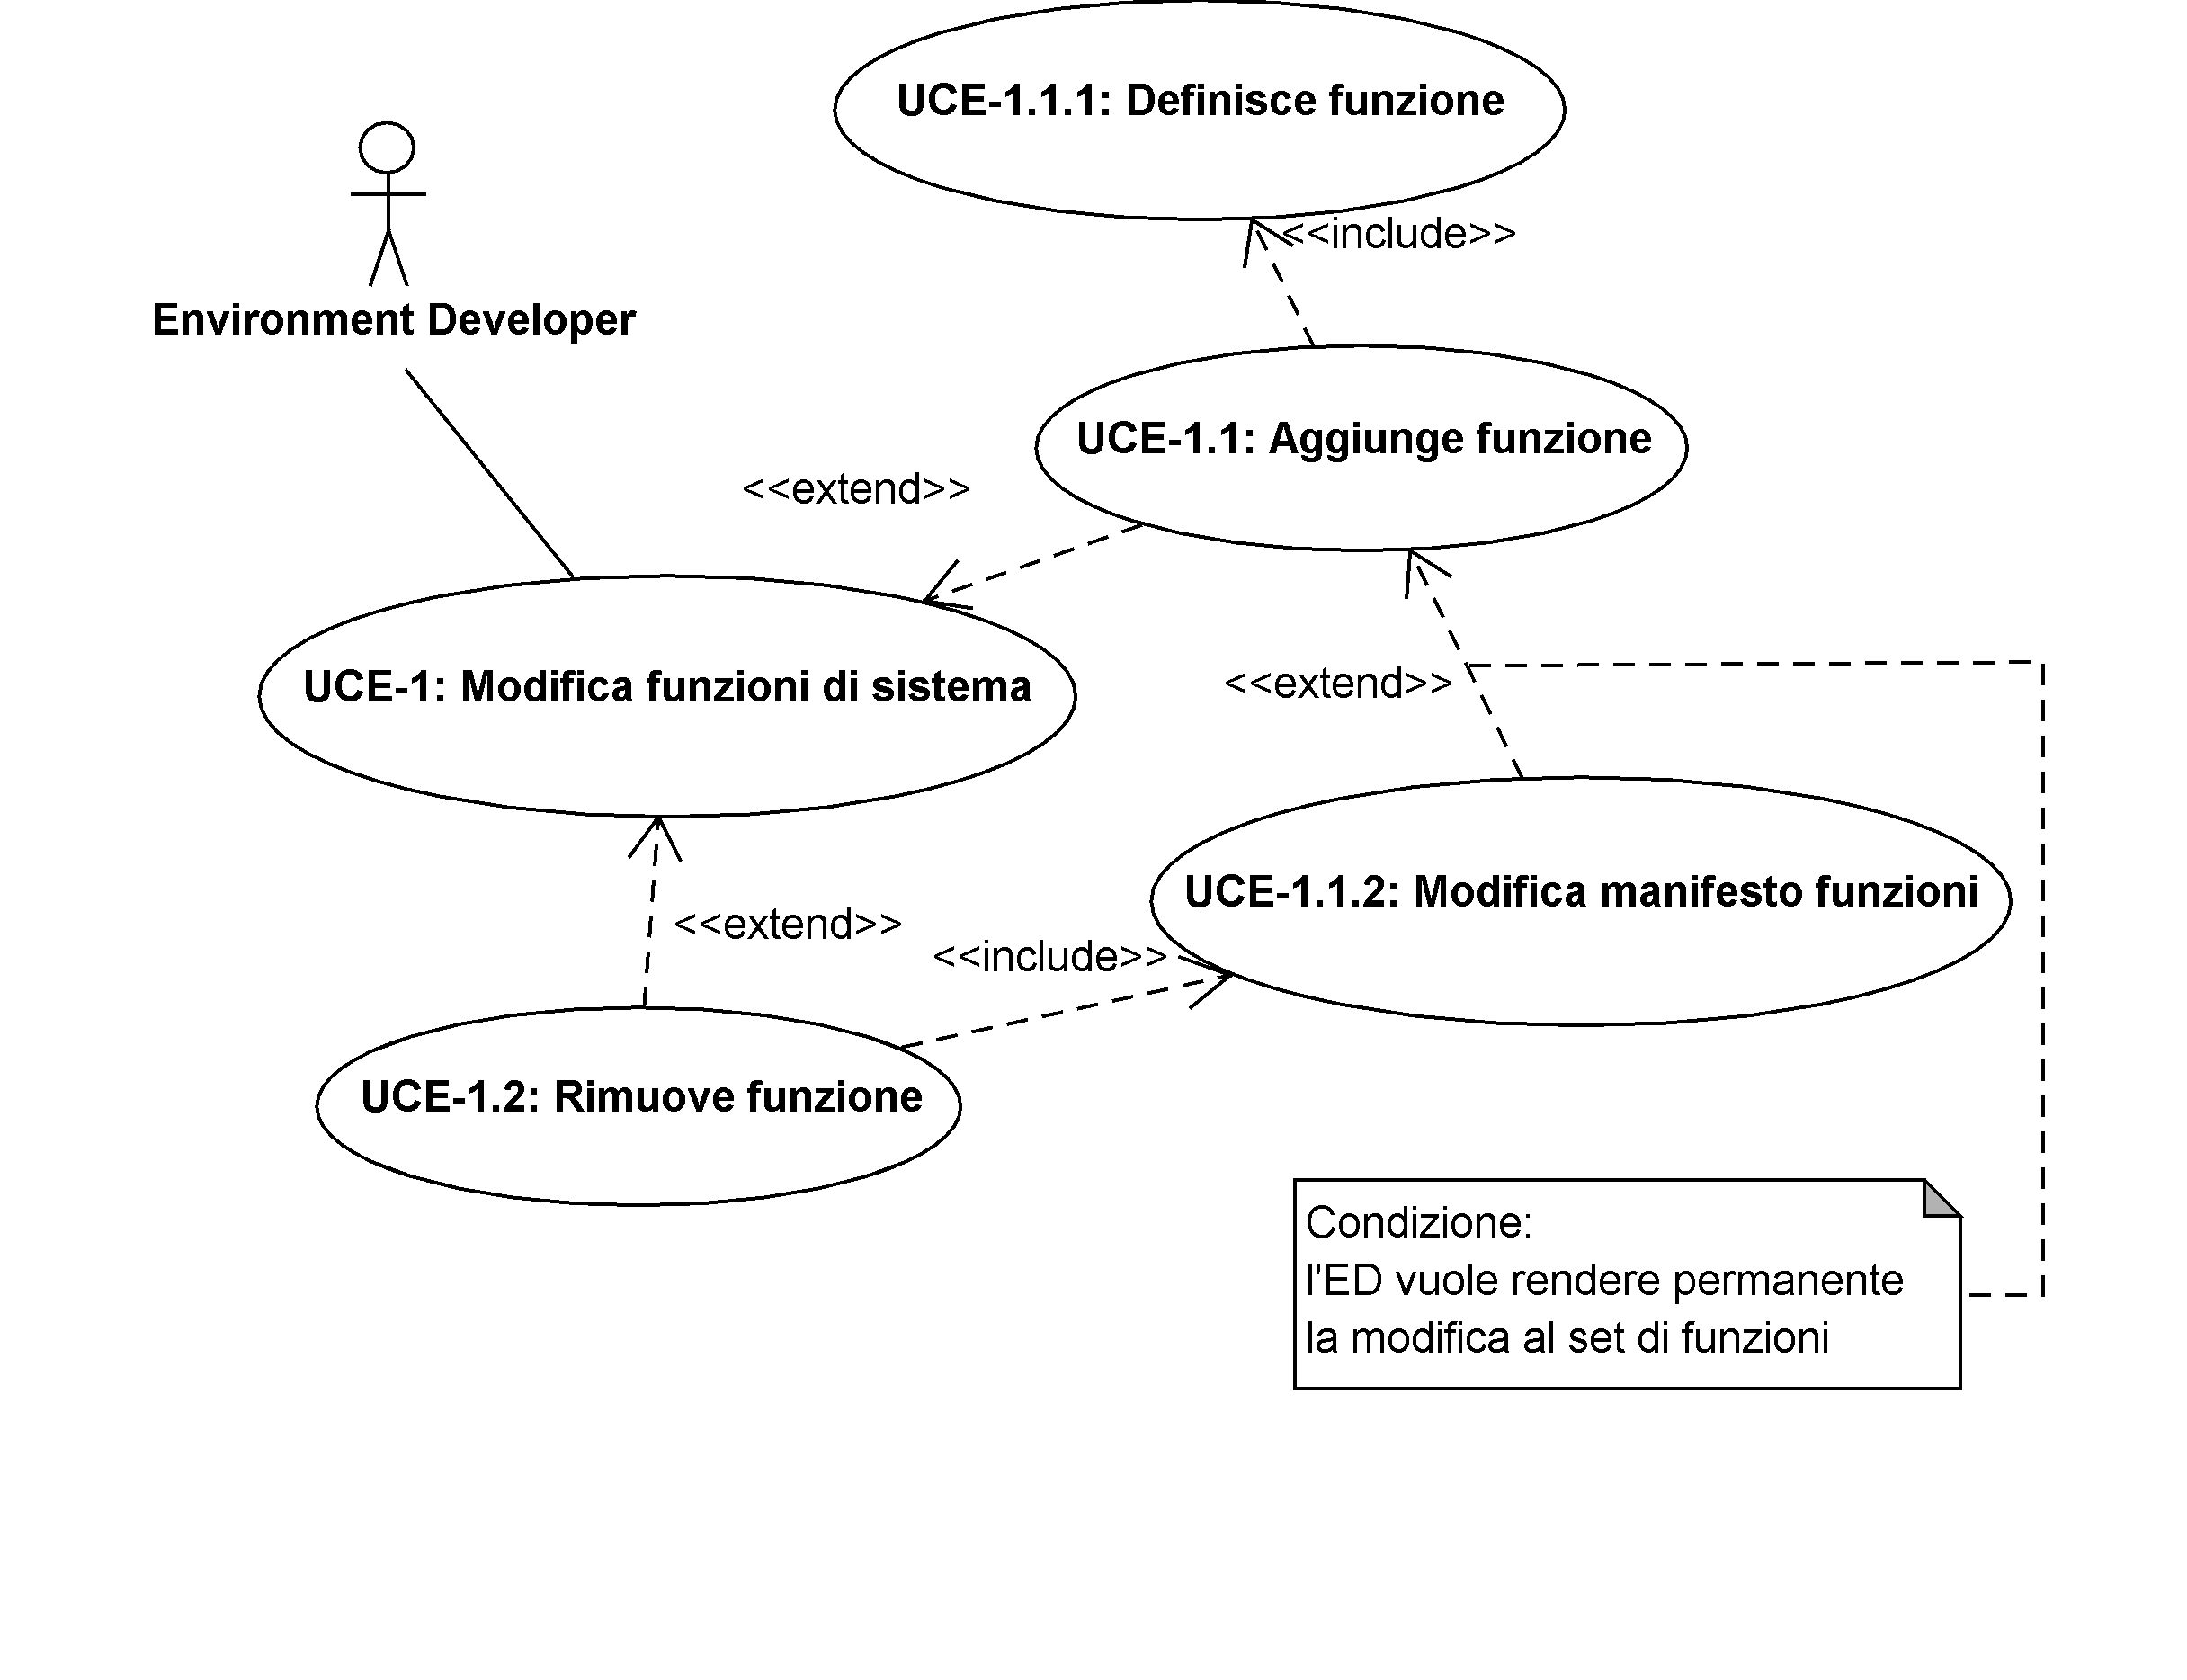
\includegraphics[width=1.1\textwidth]{Immagini/Capitolo2/UseCases/UCE-1.png}
\caption{Diagramma dei casi d'uso UCE-1}\label{fig:uc-uce-1}
\end{figure}


\begin{itemize}
	\item \textbf{Attori:} Environment Developer (\emph{ED})
	\item \textbf{Scopo e descrizione:} l'ED deve essere in grado di modificare il set di funzioni di sistema incluse nel software
	\item \textbf{Pre-condizioni:} il software fornisce meccanismi per estendere il set di funzioni di sistema
	\item \textbf{Post-condizioni:} il set di funzioni di sistema risulta modificato
	\item \textbf{Flusso principale degli eventi:}
		\begin{enumerate}
			\item l'ED esegue una modifica al set di funzioni di sistema.
			\begin{itemize}
				\item l'ED può rimuovere la definizione di una funzione esistente (si veda caso d'uso \emph{UCE-1.2})
				\item l'ED può aggiungere una nuova definizione di funzione di sistema (si veda caso d'uso \emph{UCE-1.1}).
			\end{itemize}
			\item il sistema carica il set modificato di funzioni sistema.
		\end{enumerate}
\end{itemize}


\paragraph{UCE-1.1: Aggiunge funzione}

La descrizione comprende quella del caso d'uso \emph{UCE-1.1.1}

\begin{itemize}
	\item \textbf{Attori:} ED
	\item \textbf{Scopo e descrizione:} un ED deve essere in grado di aggiungere una nuova funzione al set di funzioni di sistema.
	\item \textbf{Pre-condizioni:} il sistema è stato configurato correttamente. Il sistema non è attivo
	\item \textbf{Post-condizioni:} il sistema è attivo e una nuova funzione è disponibile nel set di funzioni di sistema
	\item \textbf{Flusso principale degli eventi:}
		\begin{enumerate}
			\item l'ED definisce il corpo di una nuova funzione di sistema (\emph{UCE-1.1.1})
			\item l'ED definisce la firma di una nuova funzione di sistema
				\begin{itemize}
					\item l'ED specifica un nome di funzione
					\item l'ED specifica un numero di parametri accettati (minimi, massimi, esatti)
					\item l'ED specifica il tipo dei parametri accettati
					\item l'ED specifica il tipo dei risultati
				\end{itemize}
			\item l'ED avvia il software
			\item l'ED richiede al software il caricamento della nuova funzione
				\begin{itemize}
					\item l'ED indica il file contenente il corpo della funzione
					\item l'ED indica la posizione della firma della funzione
				\end{itemize}
			\item la richiesta è valutata dal sistema
			\item la nuova definizione viene resa disponibile
		\end{enumerate}
	\item \textbf{Flusso alternativo \#1:}
		\begin{enumerate}
			\setcounter{enumi}{4}
			\item se l'ED ha specificato un nome di funzione già utilizzato, il sistema ignora la nuova definizione, notificando l'errore
		\end{enumerate}

	\item \textbf{Flusso alternativo \#2:}
		\begin{enumerate}
			\setcounter{enumi}{1}
			\item l'ED definisce la firma della nuova funzione indicando solo il nome e il tipo dei risultati della funzione
			\item \emph{analogo al punto 3 del flusso principale}
			\item \emph{analogo al punto 4 del flusso principale}
			\item \emph{analogo al punto 5 del flusso principale}						
			\item la firma viene integrata automaticamente dal sistema in modo che la funzione accetti un numero ed un tipo arbitrario di valori
			\item lo scenario prosegue con il punto 6 del flusso principale
		\end{enumerate}

	
\end{itemize}


\subparagraph{UCE-1.1.2: Modifica manifesto funzioni} % nome del caso d'uso SottoGruppo

\begin{itemize}
	\item \textbf{Attori:} ED
	\item \textbf{Scopo e descrizione:} ED deve essere in grado di apportare una modifica permanente al set di funzioni di sistema modificando un registro contenente l'elenco di funzioni di sistema
	\item \textbf{Pre-condizioni:} l'ED vuole rendere permanente l'aggiunta o la rimozione di una funzione di sistema. Il software non è attivo.
	\item \textbf{Post-condizioni:} il software è attivo, la modifica apportata al registro viene evidenziata nel set di funzioni di sistema disponibili
	\item \textbf{Flusso principale degli eventi:}
		\begin{enumerate}
			\item l'ED modifica il registro contenente l'elenco delle funzioni di sistema
				\begin{itemize}
					\item l'ED può aggiungere una nuova funzione all'elenco specificando il file contenente il corpo e la posizione della firma della funzione
					\item l'ED può rimuovere una funzione eliminandone le informazioni dall'elenco
				\end{itemize}
			\item l'ED salva le modifiche al registro
			\item l'ED avvia il sistema
			\item le modifiche vengono valutate dal sistema
			\item il set di funzioni disponibili viene modificato
			\item l'inizializzazione del software prosegue
		\end{enumerate}
	\item \textbf{Flusso alternativo:} 
		\begin{enumerate}
			\setcounter{enumi}{4}
			\item se l'ED ha apportato modifiche non valide al registro delle funzioni di sistema, il software notifica l'errore
			\item l'inizializzazione del software viene arrestata
		\end{enumerate}
\end{itemize}


\paragraph{UCE-1.2: Rimuove funzione}

\begin{itemize}
	\item \textbf{Attori:} ED
	\item \textbf{Scopo e descrizione:} ED deve essere in grado di rimuovere una funzione di sistema da quelle disponibili.
	\item \textbf{Pre-condizioni:} il software è configurato correttamente, il software non è attivo.
	\item \textbf{Post-condizioni:} Il software è attivo, la funzione di sistema non è presente fra quelle disponibili
	\item \textbf{Flusso principale degli eventi:}
		\begin{enumerate}
			\item l'ED modifica il manifesto delle funzioni di sistema rimuovendo le informazioni riguardanti la funzione (si guardi caso il d'uso \emph{UCE-1.1.2})
		\end{enumerate}
\end{itemize}

\pagebreak

\subsubsection{UCE-2: Monitorizza evento}

%%UCE-2: Monitorizza evento

\begin{figure}
\centering
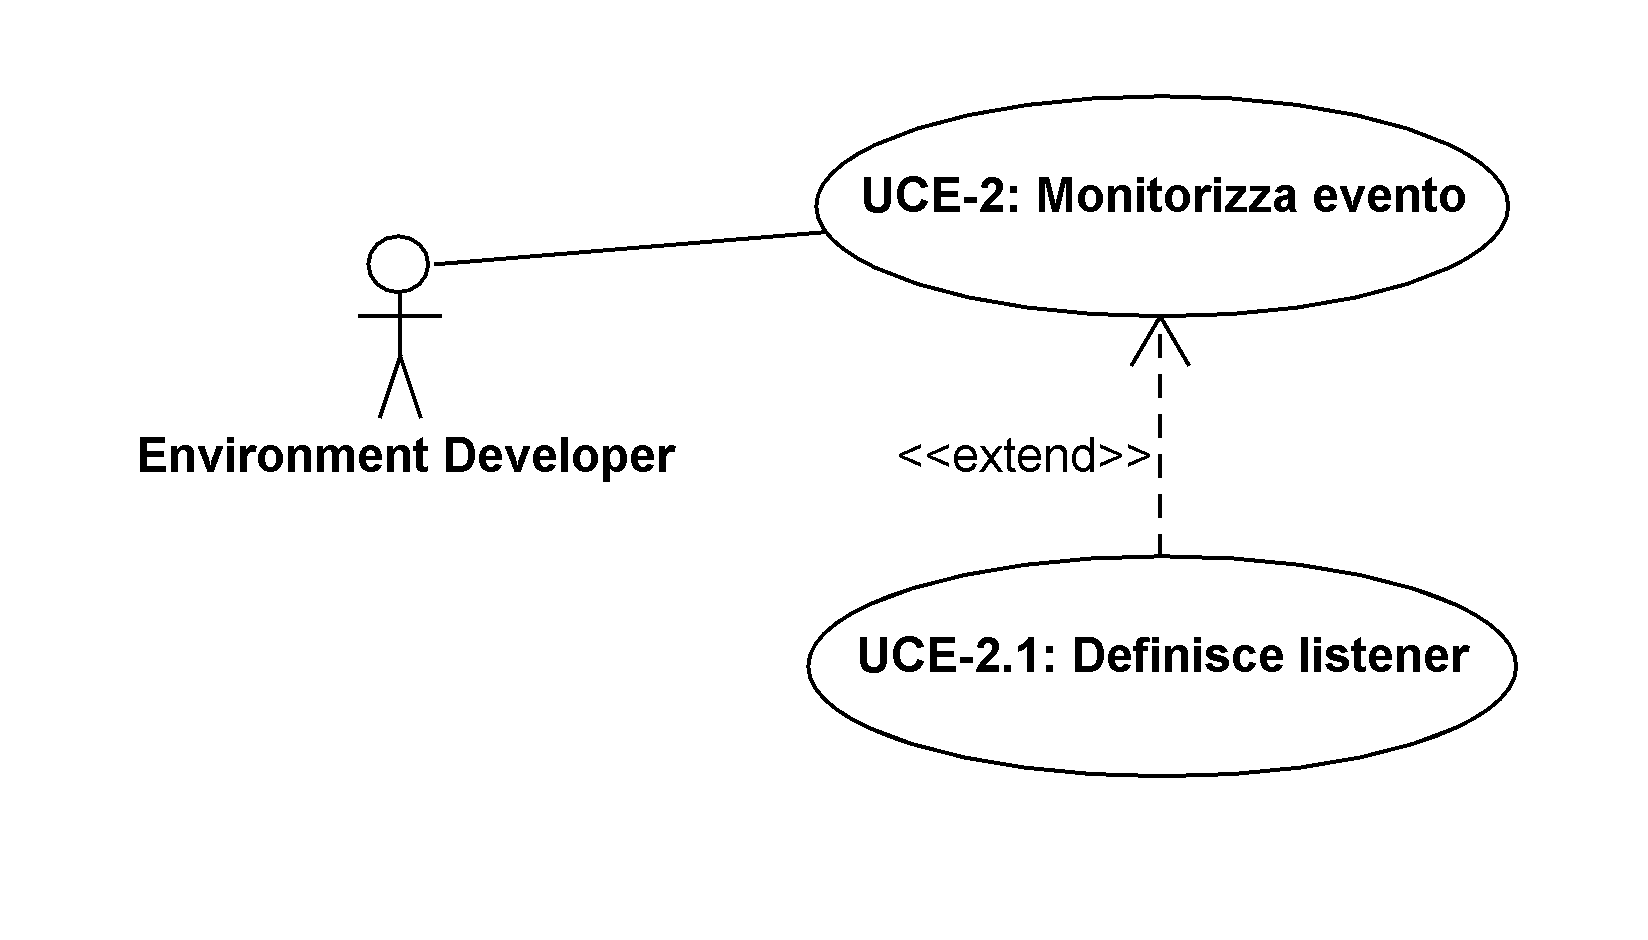
\includegraphics[width=1.1\textwidth]{Immagini/Capitolo2/UseCases/UCE-2.png}
\caption{Diagramma dei casi d'uso UCE-2}\label{fig:uc-uce-2}
\end{figure}


\begin{itemize}
	\item \textbf{Attori:} ED
	\item \textbf{Scopo e descrizione:} l'ED deve essere in grado di specificare un nuovo evento e definire un comportamento da associare al verificarsi dell'evento
	\item \textbf{Pre-condizioni:} il software fornisce meccanismi per la definizione e la notifica di un evento
	\item \textbf{Post-condizioni:} il comportamento specificato dall'ED viene eseguito al verificarsi dell'evento atteso
	\item \textbf{Flusso principale degli eventi:}
		\begin{enumerate}
			\item l'ED specifica un nuovo evento
			\item l'ED specifica un \emph{listener} che realizzi un comportamento al verificarsi di un evento (si guardi il caso d'uso \emph{UCE-2.1})
			\item l'ED avvia il sistema
			\item l'ED avvia un'elaborazione
			\item il verificarsi dell'evento provoca l'esecuzione del comportamento definito
		\end{enumerate}
\end{itemize}


\paragraph{UCE-2.1: Definisce listener}

\begin{itemize}
	\item \textbf{Attori:} ED
	\item \textbf{Scopo e descrizione:} un ED deve essere in grado di specificare un comportamento da eseguire al verificarsi di un evento
	\item \textbf{Pre-condizioni:} il sistema è stato configurato correttamente. Il sistema non è attivo
	\item \textbf{Post-condizioni:} il sistema è attivo e un comportamento è associato all'accadere di un evento
	\item \textbf{Flusso principale degli eventi:}
		\begin{enumerate}
			\item l'ED definisce un comportamento nella forma di un entità \emph{listener}
			\item l'ED registra il \emph{listener} nel sistema
		\end{enumerate}
	
\end{itemize}

\pagebreak

\subsubsection{UCE-3: Aggiunge CRS}

%%UCE-3: Aggiunge CRS

\begin{figure}
\centering
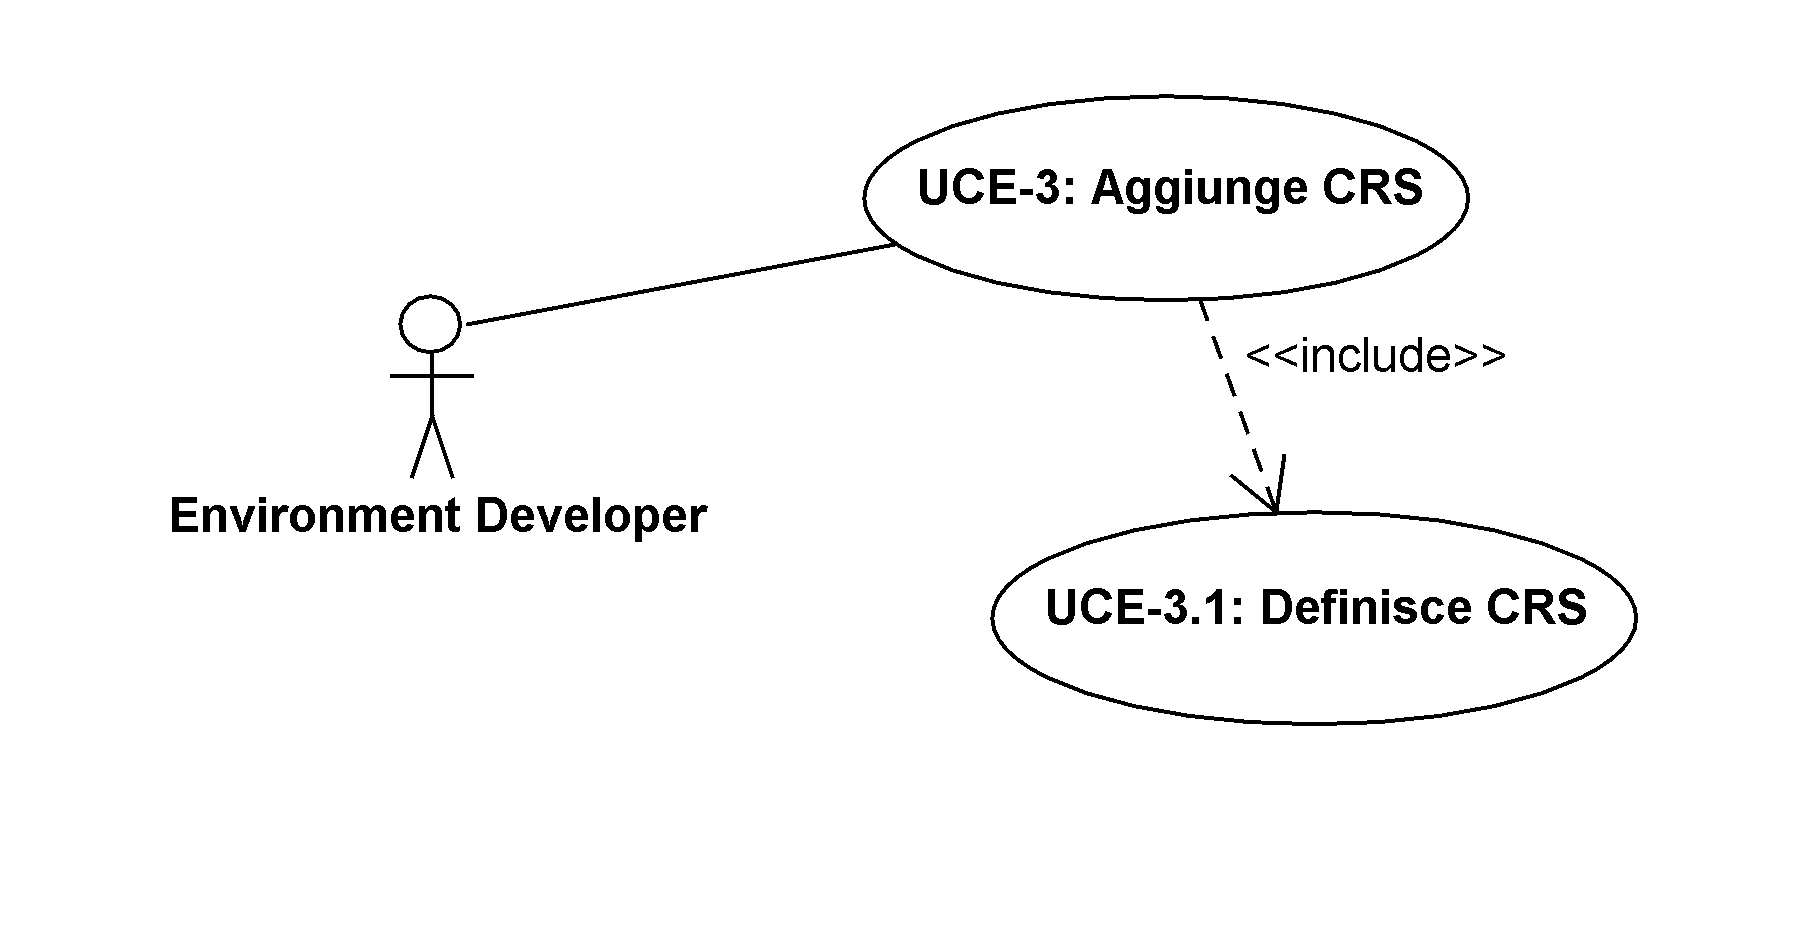
\includegraphics[width=1.1\textwidth]{Immagini/Capitolo2/UseCases/UCE-3.png}
\caption{Diagramma dei casi d'uso UCE-3}\label{fig:uc-uce-3}
\end{figure}


\begin{itemize}
	\item \textbf{Attori:} ED
	\item \textbf{Scopo e descrizione:} l'ED deve essere in grado di definire ed aggiungere una nuova \emph{strategia di risoluzione dei conflitti} (CRS)
	\item \textbf{Pre-condizioni:} il software fornisce meccanismi per la definizione e l'aggiunta di CRS, il sistema non è attivo
	\item \textbf{Post-condizioni:} il sistema è attivo e la una nuova CRS è disponibile
	\item \textbf{Flusso principale degli eventi:}
		\begin{enumerate}
			\item l'ED definisce una nuova CRS attraverso i meccanismi previsti dal sistema (si guardi il caso d'uso \emph{UCE-3.1})
			\item l'ED aggiunge la nuova CRS al sistema
			\item l'ED avvia il sistema
		\end{enumerate}
\end{itemize}


\paragraph{UCE-3.1: Definisce CRS}

\begin{itemize}
	\item \textbf{Attori:} ED
	\item \textbf{Scopo e descrizione:} l'ED deve essere in grado di definire una nuova CRS
	\item \textbf{Pre-condizioni:} il sistema è stato configurato correttamente. Il sistema non è attivo. Il sistema offre meccanismi per la definizione di una nuova CRS.
	\item \textbf{Post-condizioni:} una nuova CRS è disponibile per l'integrazione al sistema
	\item \textbf{Flusso principale degli eventi:}
		\begin{enumerate}
			\item l'ED definisce una nuova CRS
			\item l'ED realizza la CRS in una unità di elaborazione separata e raggiungibile al software
		\end{enumerate}
	
\end{itemize}

\pagebreak

\subsubsection{UCE-4: Testa environment}

%%UCE-4: Testa environment

\begin{figure}
\centering
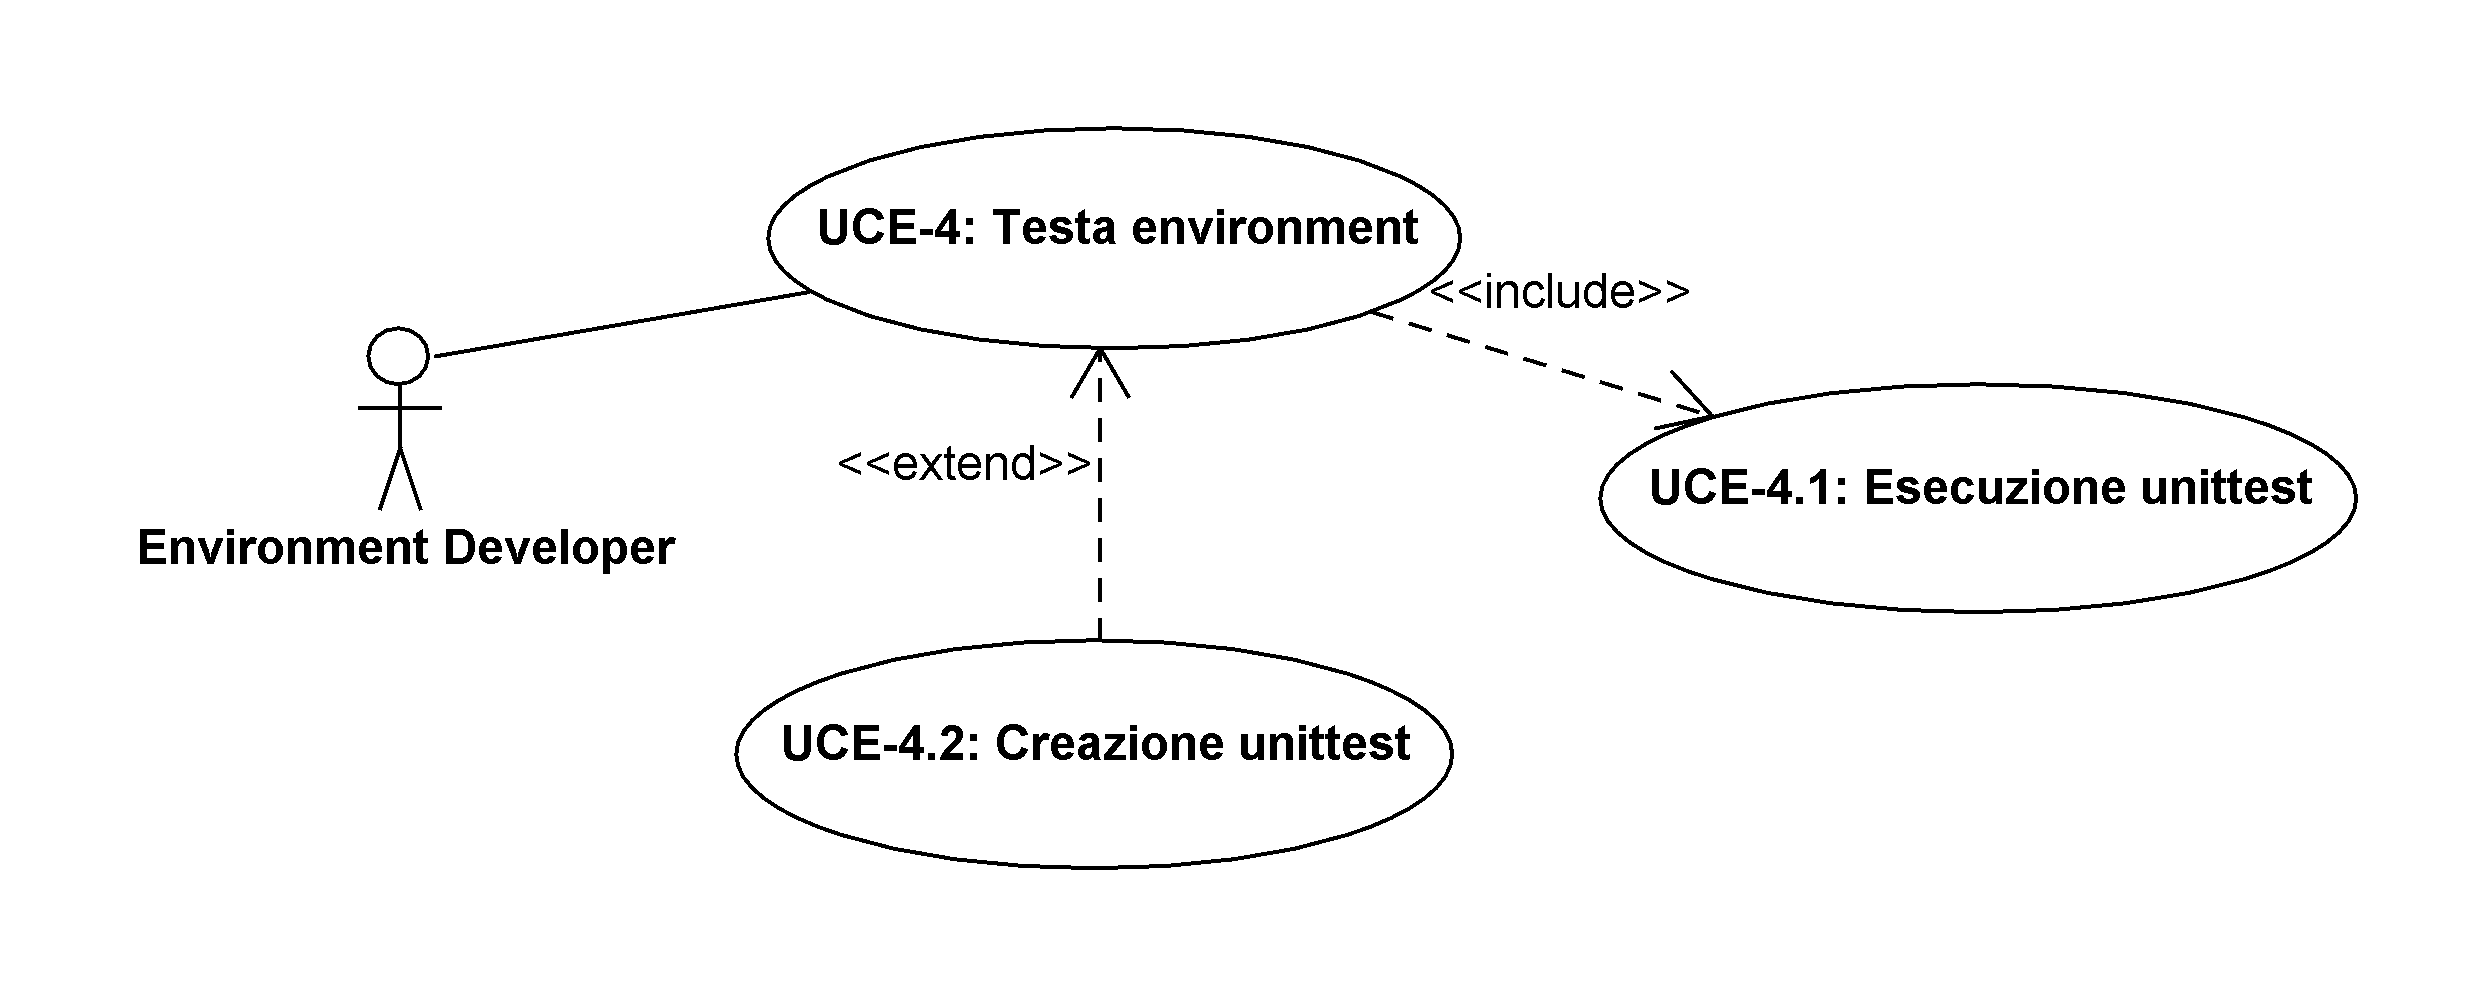
\includegraphics[width=1.1\textwidth]{Immagini/Capitolo2/UseCases/UCE-4.png}
\caption{Diagramma dei casi d'uso UCE-4}\label{fig:uc-uce-4}
\end{figure}

La descrizione comprende quella del caso d'uso \emph{UCE-4.1}.

\begin{itemize}
	\item \textbf{Attori:} ED
	\item \textbf{Scopo e descrizione:} l'ED deve essere in grado di verificare il funzionamento dell'environment utilizzando dei test d'unità. L'ED deve avere la possibilità di realizzare dei test d'unità per le funzionalità aggiunte
	\item \textbf{Pre-condizioni:} il software fornisce meccanismi per l'esecuzione di test d'unità in grado di verificare il comportamento dei componenti di sistema. Il software fornisce un framework per la definizione di nuovi test d'unità per le funzionalità introdotte
	\item \textbf{Post-condizioni:} l'ED ottiene dal software un riepilogo sul funzionamento delle componenti
	\item \textbf{Flusso principale degli eventi:}
		\begin{enumerate}
			\item l'ED avvia l'esecuzione dei test d'unità (\emph{UCE-4.1})
			\item l'ED ottiene un riepilogo dei risultati dei test
				\begin{itemize}
					\item il riepilogo indica eventuali test falliti
					\item il riepilogo indica il motivo del fallimento dei test
				\end{itemize}
		\end{enumerate}
\end{itemize}


\paragraph{UCE-4.1: Creazione unittest}

\begin{itemize}
	\item \textbf{Attori:} ED
	\item \textbf{Scopo e descrizione:} l'ED deve avere la possibilità di definire ed eseguire test d'unità in grado di verificare il corretto funzionamento delle caratteristiche aggiunte
	\item \textbf{Pre-condizioni:} il sistema è stato configurato correttamente. Il software offre meccanismi per l'integrazione di nuovi test d'unità a quelli forniti con il sistema
	\item \textbf{Post-condizioni:} un nuovo test d'unità è integrato con quelli forniti dal sistema
	\item \textbf{Flusso principale degli eventi:}
		\begin{enumerate}
			\item l'ED realizza un nuovo test d'unità
			\item l'ED registra il nuovo test d'unità insieme a quelli forniti dal software
		\end{enumerate}
\end{itemize}

\pagebreak

\subsubsection{UCA-1: Avvia Server}

%%UCA-1: Avvia server

\begin{itemize}
	\item \textbf{Attori:} Server Administrator
	\item \textbf{Scopo e descrizione:} il Server Administrator deve essere in inizializzare un'istanza server del software
	\item \textbf{Pre-condizioni:} il sistema è correttamente configurato. Il software è correttamente configurato
	\item \textbf{Post-condizioni:} un'istanza server del software è attiva e attende connessioni
	\item \textbf{Flusso principale degli eventi:}
		\begin{enumerate}
			\item il Server Administrator avvia un'istanza del software
			\item la configurazione del software viene valutata (si guardi caso d'uso \emph{UCA-3})
		\end{enumerate}
	\item \textbf{Flusso alternativo \#1:}
		\begin{enumerate}
			\setcounter{enumi}{1}
			\item se una specifica di configurazione non è disponibile, il software notifica l'errore
			\item vengono utilizzati dei parametri di default
		\end{enumerate}
	\item \textbf{Flusso alternativo \#2:}
		\begin{enumerate}
			\setcounter{enumi}{1}
			\item se la specifica di configurazione non è valida, il software notifica l'errore
			\item l'esecuzione viene terminata
		\end{enumerate}
\end{itemize}
\pagebreak

\subsubsection{UCA-2: Arresta Server}

%%UCA-2: Arresta Server

\begin{itemize}
	\item \textbf{Attori:} Server Administrator
	\item \textbf{Scopo e descrizione:} il Server Administrator deve essere in terminare l'esecuzione di un'istanza del software
	\item \textbf{Pre-condizioni:} un'istanza del software è attiva
	\item \textbf{Post-condizioni:} l'istanza del software non è più attiva
	\item \textbf{Flusso principale degli eventi:}
		\begin{enumerate}
			\item il Server Administrator richiede l'arresto del software
			\item tutte le sessioni vengono chiuse
			\item il software viene arrestato
		\end{enumerate}
	\item \textbf{Flusso alternativo:}
		\begin{enumerate}
			\setcounter{enumi}{1}
			\item se si verifica un errore durante la chiusura di una sessione (o un tempo limite per l'operazione viene superato), la sessione viene distrutta forzatamente
			\item lo scenario prosegue dal punto 3 del flusso principale
		\end{enumerate}
\end{itemize}
\pagebreak

\subsubsection{UCA-3: Configura Server}

%%UCA-3: Configura Server

\begin{figure}
\centering
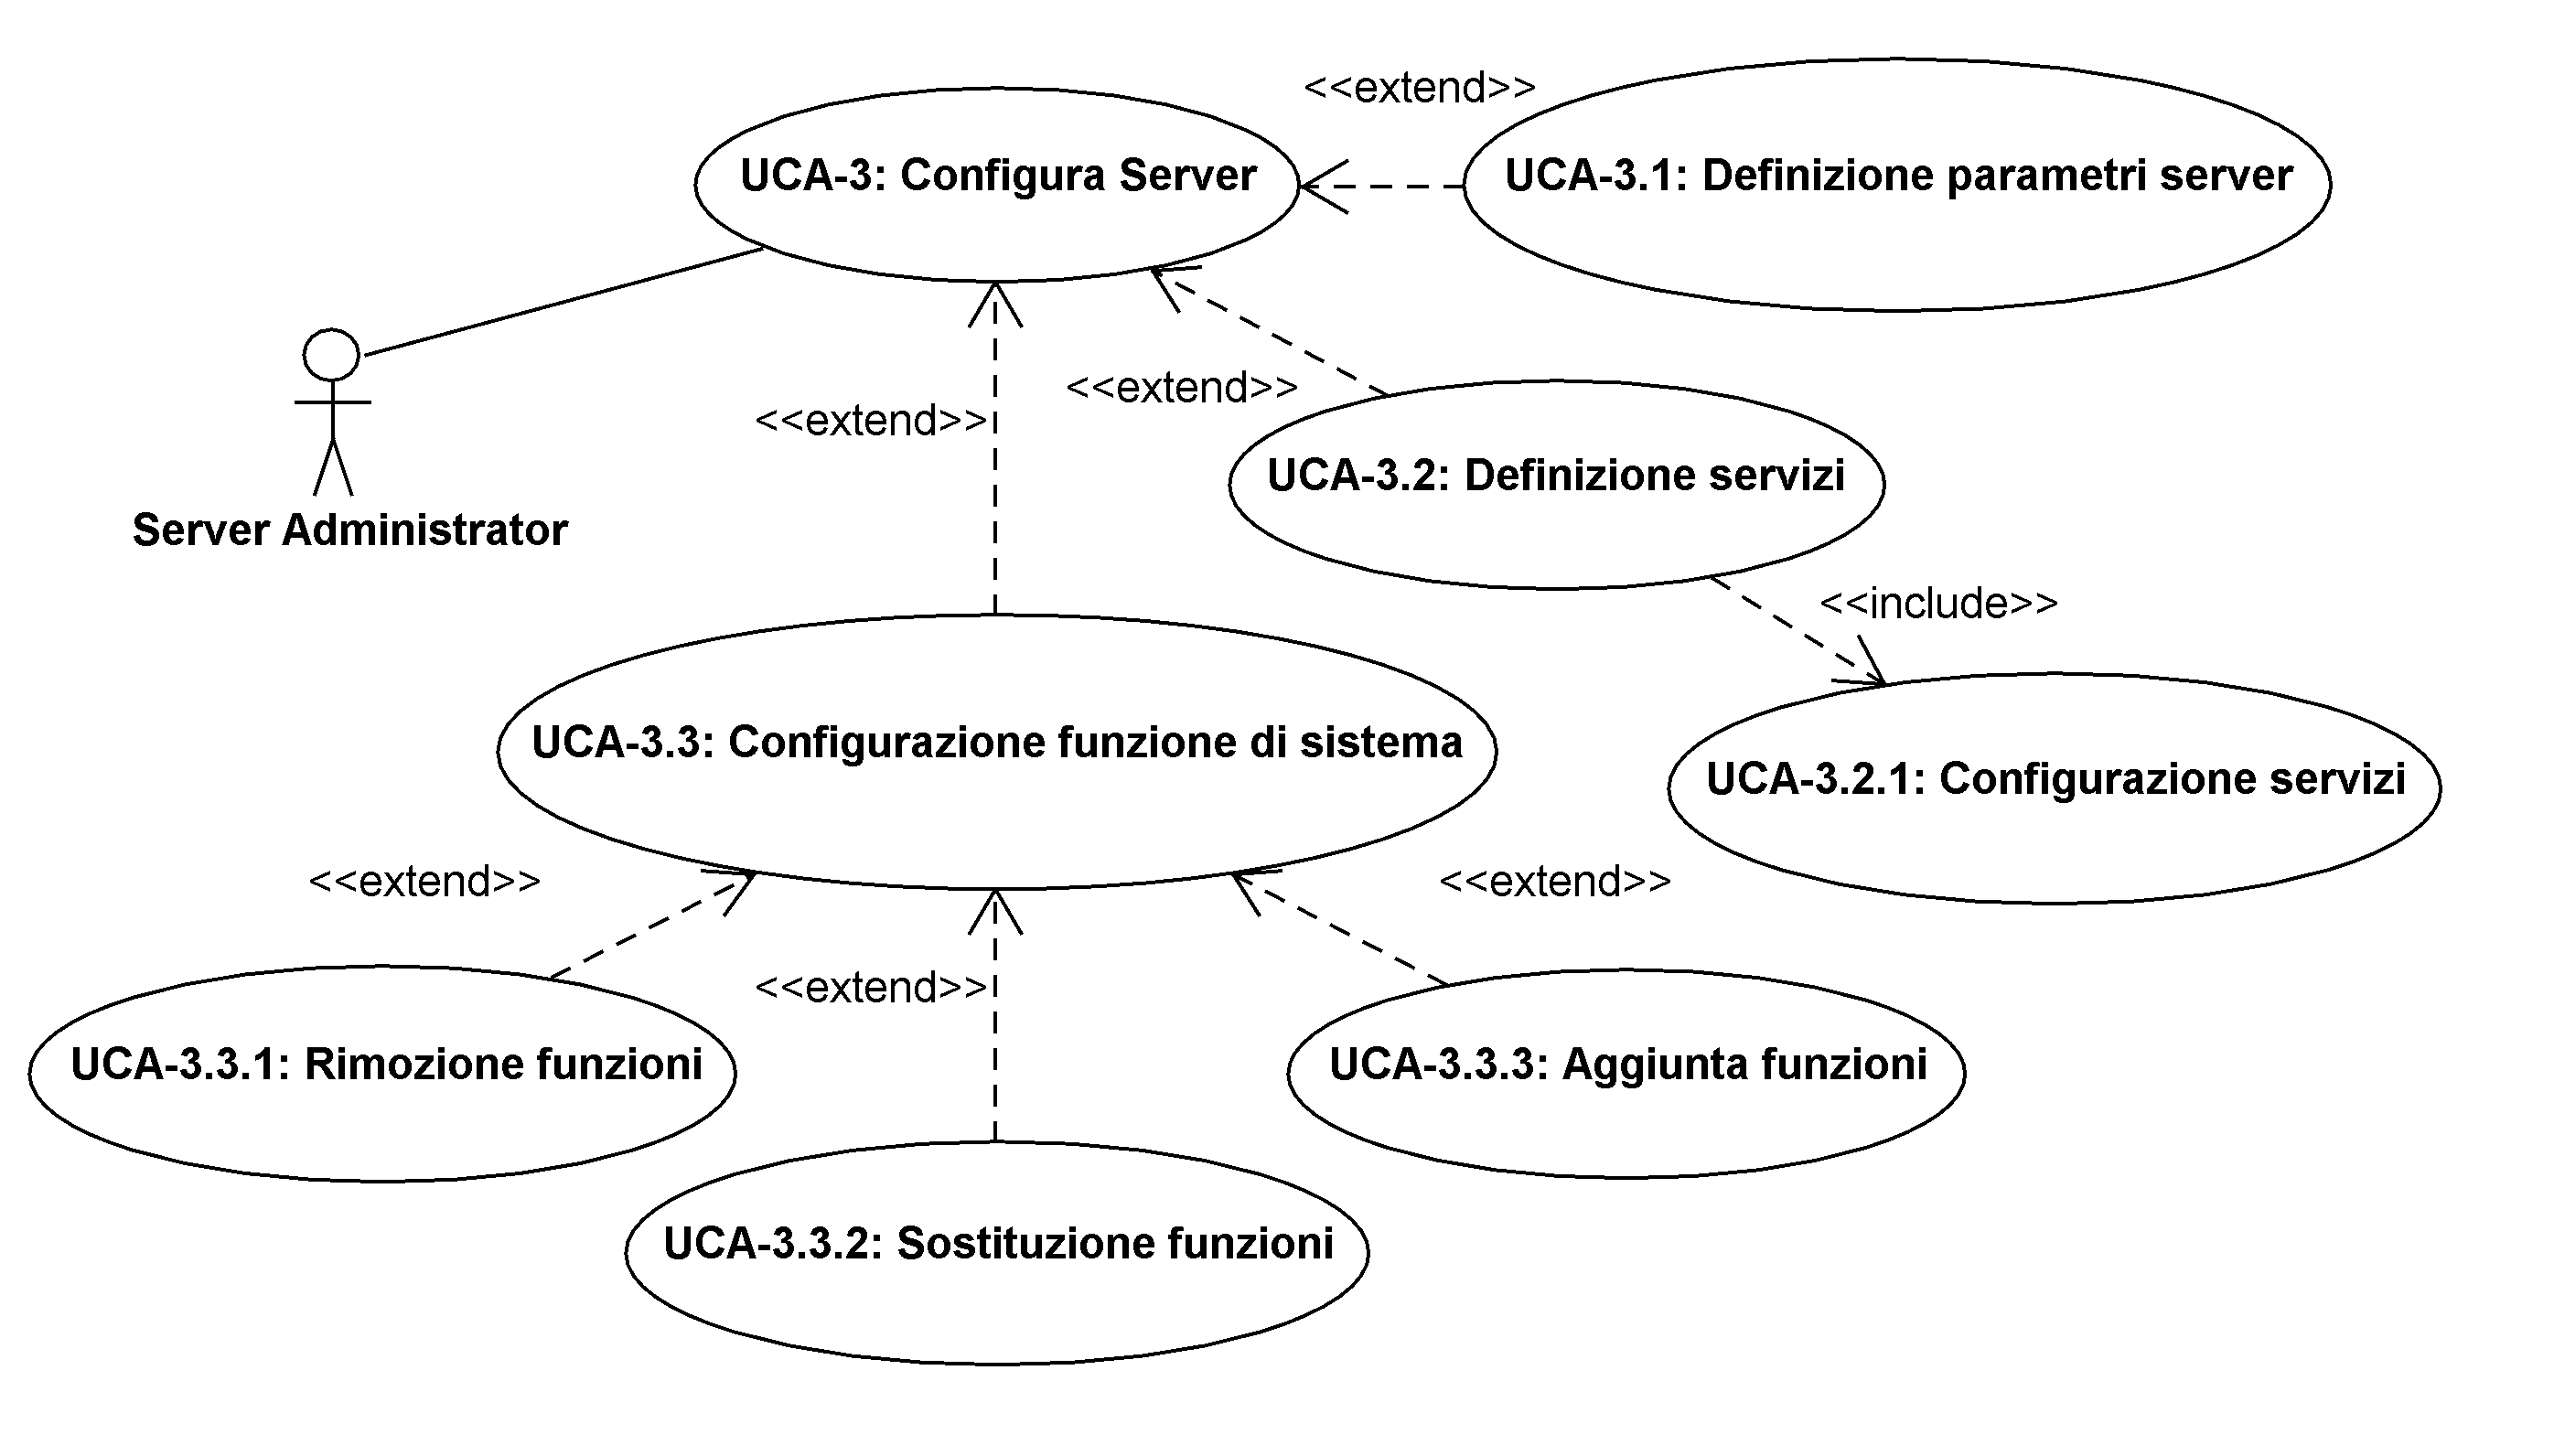
\includegraphics[width=1.1\textwidth]{Immagini/Capitolo2/UseCases/UCA-3.png}
\caption{Diagramma dei casi d'uso UCA-3}\label{fig:uc-uca-3}
\end{figure}

\begin{itemize}
	\item \textbf{Attori:} Server Administrator
	\item \textbf{Scopo e descrizione:} il Server Administrator deve avere la possibilità di configurare le funzioni del software MyCLIPS utilizzabili dai client, i servizi offerti dal server e i parametri di base del modulo server attraverso un file di configurazione
	\item \textbf{Pre-condizioni:} il sistema offre un formato di specifica delle configurazioni e un meccanismo di caricamento delle stesse
	\item \textbf{Post-condizioni:} il funzionamento del software rispecchia i parametri definiti del file di configurazione
	\item \textbf{Flusso principale degli eventi:}
		\begin{enumerate}
			\item il Server Administrator apre il file di configurazione attraverso un programma di \emph{text-editing}
			\item il Server Administrator modifica i parametri di configurazione del server
				\begin{itemize}
					\item il Server Administrator modifica le funzioni di MyCLIPS utilizzabili dai client (si guardi il caso d'uso \emph{UCA-3.3})
					\item il Server Administrator modifica i servizi attivi offerti dal server (si guardi il caso d'uso \emph{UCA-3.2})
					\item il Server Administrator modifica i parametri di base del server (si guardi il caso d'uso \emph{UCA-3.1})
				\end{itemize}
			\item il Server Administrator salva le modifiche
		\end{enumerate}
\end{itemize}


\paragraph{UCA-3.1: Configurazione parametri server}

\begin{itemize}
	\item \textbf{Attori:} Server Administrator
	\item \textbf{Scopo e descrizione:} il Server Administrator deve avere la possibilità di modificare i parametri di configurazione di base del server
	\item \textbf{Pre-condizioni:} \emph{nessuna}
	\item \textbf{Post-condizioni:} i parametri di configurazione risultano modificati secondo le aspettative del Server Administrator
	\item \textbf{Flusso principale degli eventi:}
		\begin{enumerate}
			\item il Server Administrator modifica i parametri di base del server. Può configurare:
				\begin{itemize}
					\item l'indirizzo di ascolto (\emph{bind-address})
					\item la porta di ascolto (\emph{bind-port})
					\item la creazione di un registro delle richieste (\emph{log-requests})
					\item il livello di dettaglio del registro delle richieste (\emph{log-level})
				\end{itemize}
		\end{enumerate}
\end{itemize}


\paragraph{UCA-3.2: Definizione servizi}

La descrizione comprende anche quella del caso d'uso \emph{UCA-3.2.1}.

\begin{itemize}
	\item \textbf{Attori:} Server Administrator
	\item \textbf{Scopo e descrizione:} il Server Administrator deve avere la possibilità di definire i servizi attivi offerti dal server e configurare i parametri di funzionamento dei servizi
	\item \textbf{Pre-condizioni:} \emph{nessuna}
	\item \textbf{Post-condizioni:} i parametri di configurazione risultano modificati secondo le aspettative del Server Administrator
	\item \textbf{Flusso principale degli eventi:}
		\begin{enumerate}
			\item il Server Administrator modifica i servizi attivi offerti dal server specificando:
				\begin{itemize}
					\item l'interfaccia offerta dal servizio
					\item un'implementazione del servizio
				\end{itemize}
			\item il Server Administrator specifica i parametri relativi ai servizi attivi (\emph{UCA-3.2.1)}: il formato, il tipo e i valori delle configurazioni sono definite dalla specifica implementazione del servizio
		\end{enumerate}
\end{itemize}





\pagebreak

\subsubsection{UCS-1: Analisi dei risultati}

%%UCS-1: Analisi dei risultati

\begin{figure}
\centering
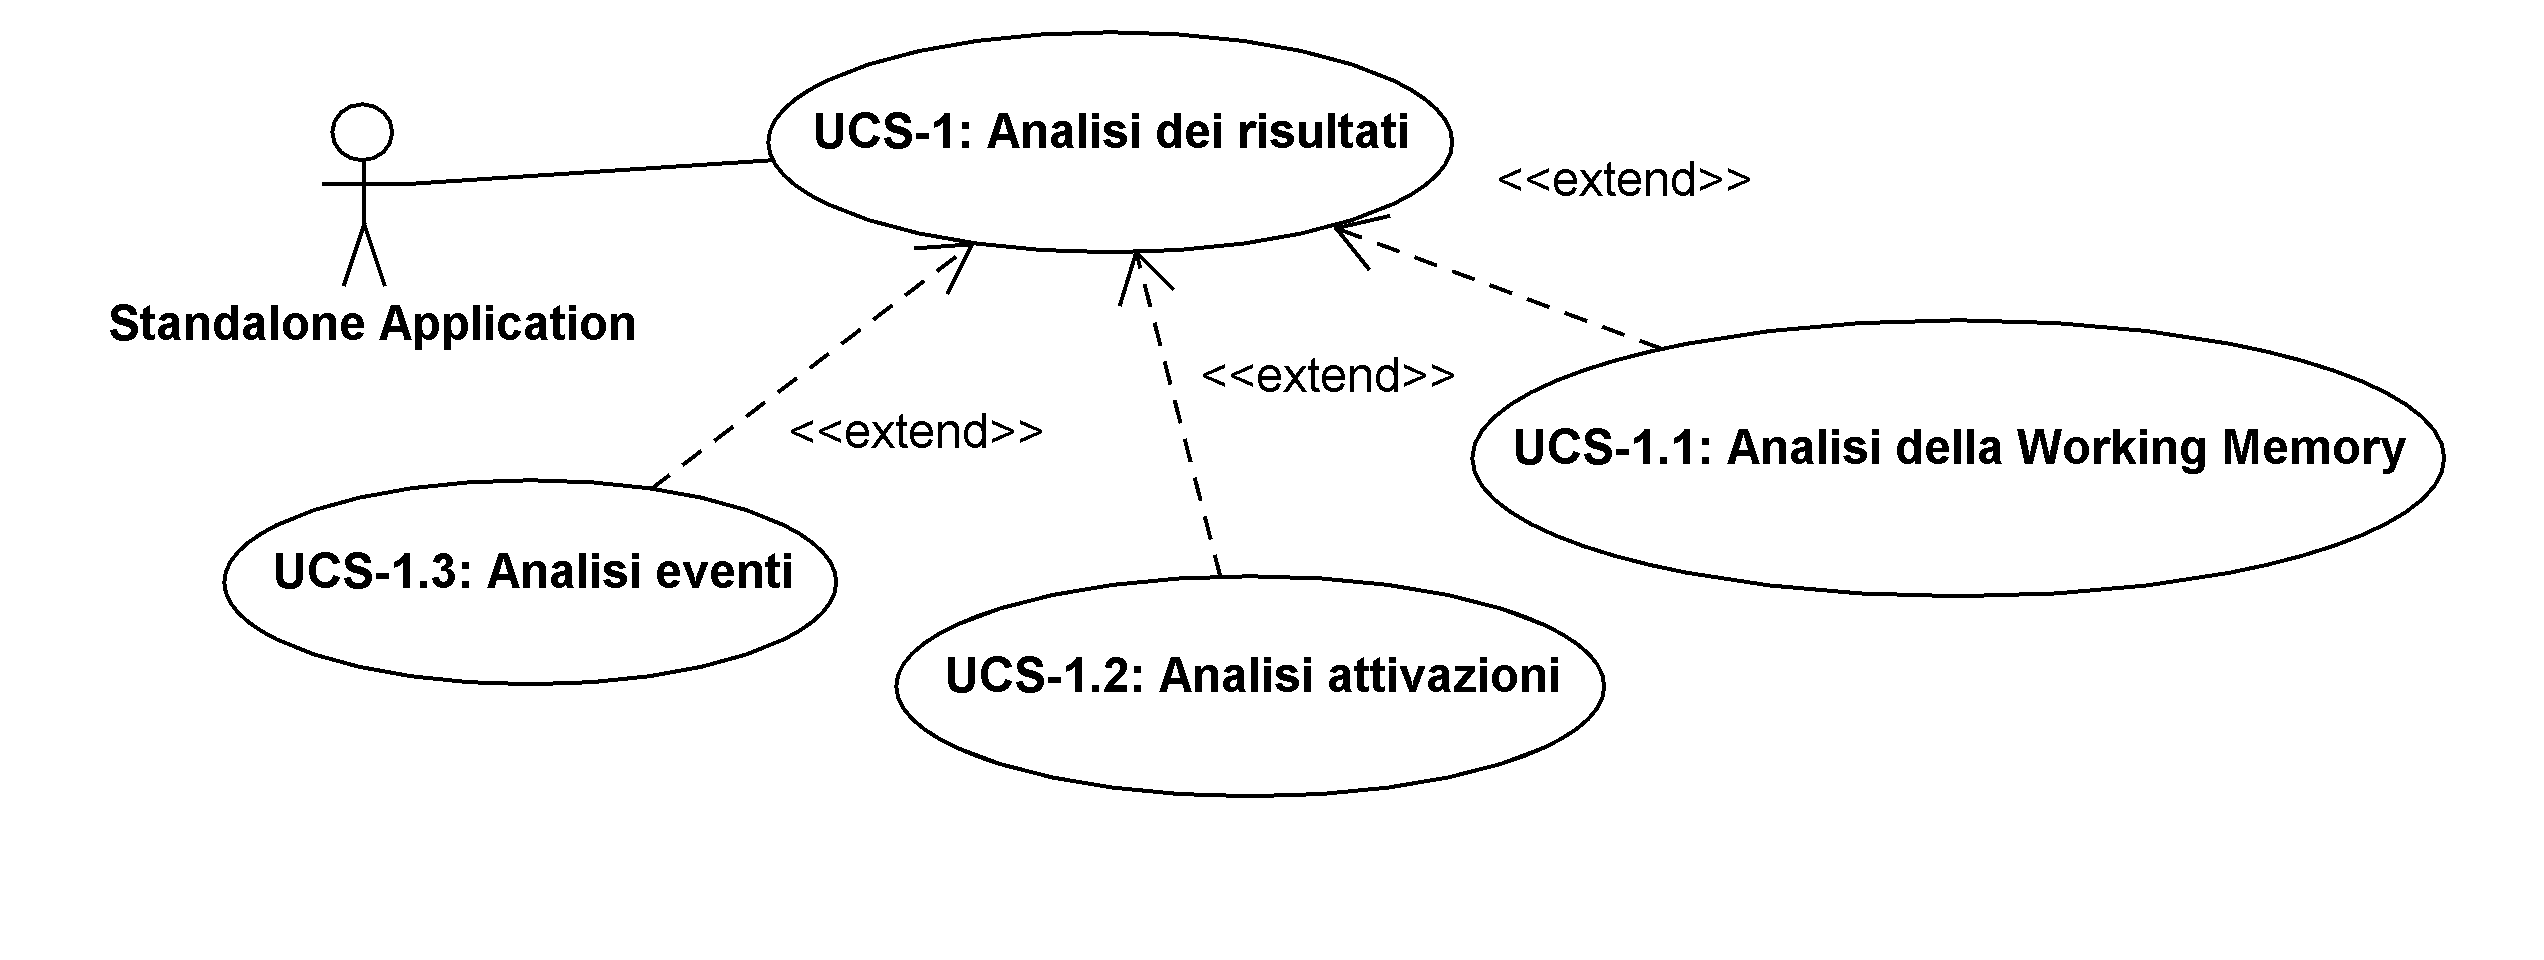
\includegraphics[width=1.1\textwidth]{Immagini/Capitolo2/UseCases/UCS-1.png}
\caption{Diagramma dei casi d'uso UCS-1}\label{fig:uc-ucs-1}
\end{figure}

\begin{itemize}
	\item \textbf{Attori:} Standalone Application
	\item \textbf{Scopo e descrizione:} la Standalone Application deve avere la possibilità di accedere alle informazioni riguardanti lo stato finale di un'elaborazione eseguita dal software e ricevere notifica del verificarsi di eventi durante l'elaborazione
	\item \textbf{Pre-condizioni:} la Standalone Application ha eseguito con successo il caso d'uso \emph{UCC-1.2}
	\item \textbf{Post-condizioni:} la Standalone Application ha ottenuto le informazioni necessarie
	\item \textbf{Flusso principale degli eventi:}
		\begin{enumerate}
			\item la Standalone Application richiede informazioni sullo stato terminale di elaborazione del software
				\begin{itemize}
					\item la Standalone Application richiede informazioni sullo stato della \emph{working-memory} (si guardi il caso d'uso \emph{UCS-1.1})
					\item la Standalone Application richiede informazioni sullo stato delle attivazioni ancora presenti (si guardi il caso d'uso \emph{UCS-1.2})
					\item la Standalone Application valuta il verificarsi di un evento (si guardi il caso d'uso \emph{UCS-1.3})
				\end{itemize}
			\item la Standalone Application ottiene le informazioni richieste
		\end{enumerate}
\end{itemize}


\paragraph{UCS-1.1: Analisi della Working-Memory}

\begin{itemize}
	\item \textbf{Attori:} Standalone Application
	\item \textbf{Scopo e descrizione:} la Standalone Application deve avere accesso alle informazioni presenti nella \emph{Working Memory}
	\item \textbf{Pre-condizioni:} la Standalone Application ha eseguito con successo il caso d'uso \emph{UCC-1.2}
	\item \textbf{Post-condizioni:} la Standalone Application ottiene le informazioni sui fatti presenti nella \emph{Working Memory}
	\item \textbf{Flusso principale degli eventi:}
		\begin{enumerate}
			\item la Standalone Application richiede una vista dei dati presenti nella \emph{Working Memory}
				\begin{itemize}
					\item la Standalone Application può limitare la ricerca solo ai fatti relativi ad un sottogruppo dei moduli specificati
					\item la Standalone Application può richiedere tutti i fatti presenti nella \emph{Working Memory}
				\end{itemize}
			\item la Standalone Application ottiene l'elenco dei fatti richiesti
		\end{enumerate}
\end{itemize}


\paragraph{UCS-1.2: Analisi attivazioni}

\begin{itemize}
	\item \textbf{Attori:} Standalone Application
	\item \textbf{Scopo e descrizione:} la Standalone Application deve avere accesso alle informazioni presenti nell'agenda delle attivazioni
	\item \textbf{Pre-condizioni:} la Standalone Application ha eseguito con successo il caso d'uso \emph{UCC-1.1}
	\item \textbf{Post-condizioni:} la Standalone Application ottiene l'elenco di attivazioni disponibili nell'agenda delle attivazioni nelle modalità che ha indicato
	\item \textbf{Flusso principale degli eventi:}
		\begin{enumerate}
			\item la Standalone Application richiede una vista sulle attivazioni presenti nell'agenda delle attivazioni.
				\begin{itemize}
					\item la Standalone Application può limitare la ricerca solo alle attivazioni relative ad un sottogruppo dei moduli specificati
					\item la Standalone Application può richiedere l'intera lista delle attivazioni presenti in agenda
				\end{itemize}
			\item la Standalone Application ottiene l'elenco delle attivazioni richieste
		\end{enumerate}
\end{itemize}


\paragraph{UCS-1.3: Analisi eventi}

\begin{itemize}
	\item \textbf{Attori:} Standalone Application
	\item \textbf{Scopo e descrizione:} la Standalone Application deve ricevere notifica del verificarsi di un evento per il quale ha espresso interesse nelle modalità previste dal software
	\item \textbf{Pre-condizioni:} la Standalone Application ha eseguito con successo il caso d'uso \emph{UCC-1.2.3}
	\item \textbf{Post-condizioni:} la Standalone Application ha eseguito il comportamento associato ad un determinato evento
	\item \textbf{Flusso principale degli eventi:}
		\begin{enumerate}
			\item la Standalone Application esprime interesse relativamente al verificarsi di un evento (si guardi caso d'uso \emph{UCC-1.2.3})
			\item la Standalone Application osserva la notifica del verificarsi di un evento
			\item la Standalone Application analizza i parametri relativi all'evento
			\item la Standalone Application esegue il comportamento associato all'evento con i parametri forniti
		\end{enumerate}
\end{itemize}





\pagebreak

\subsubsection{UCR-1: Inizializza sessione}

%%UCR-1: Inizializza sessione

\begin{figure}
\centering
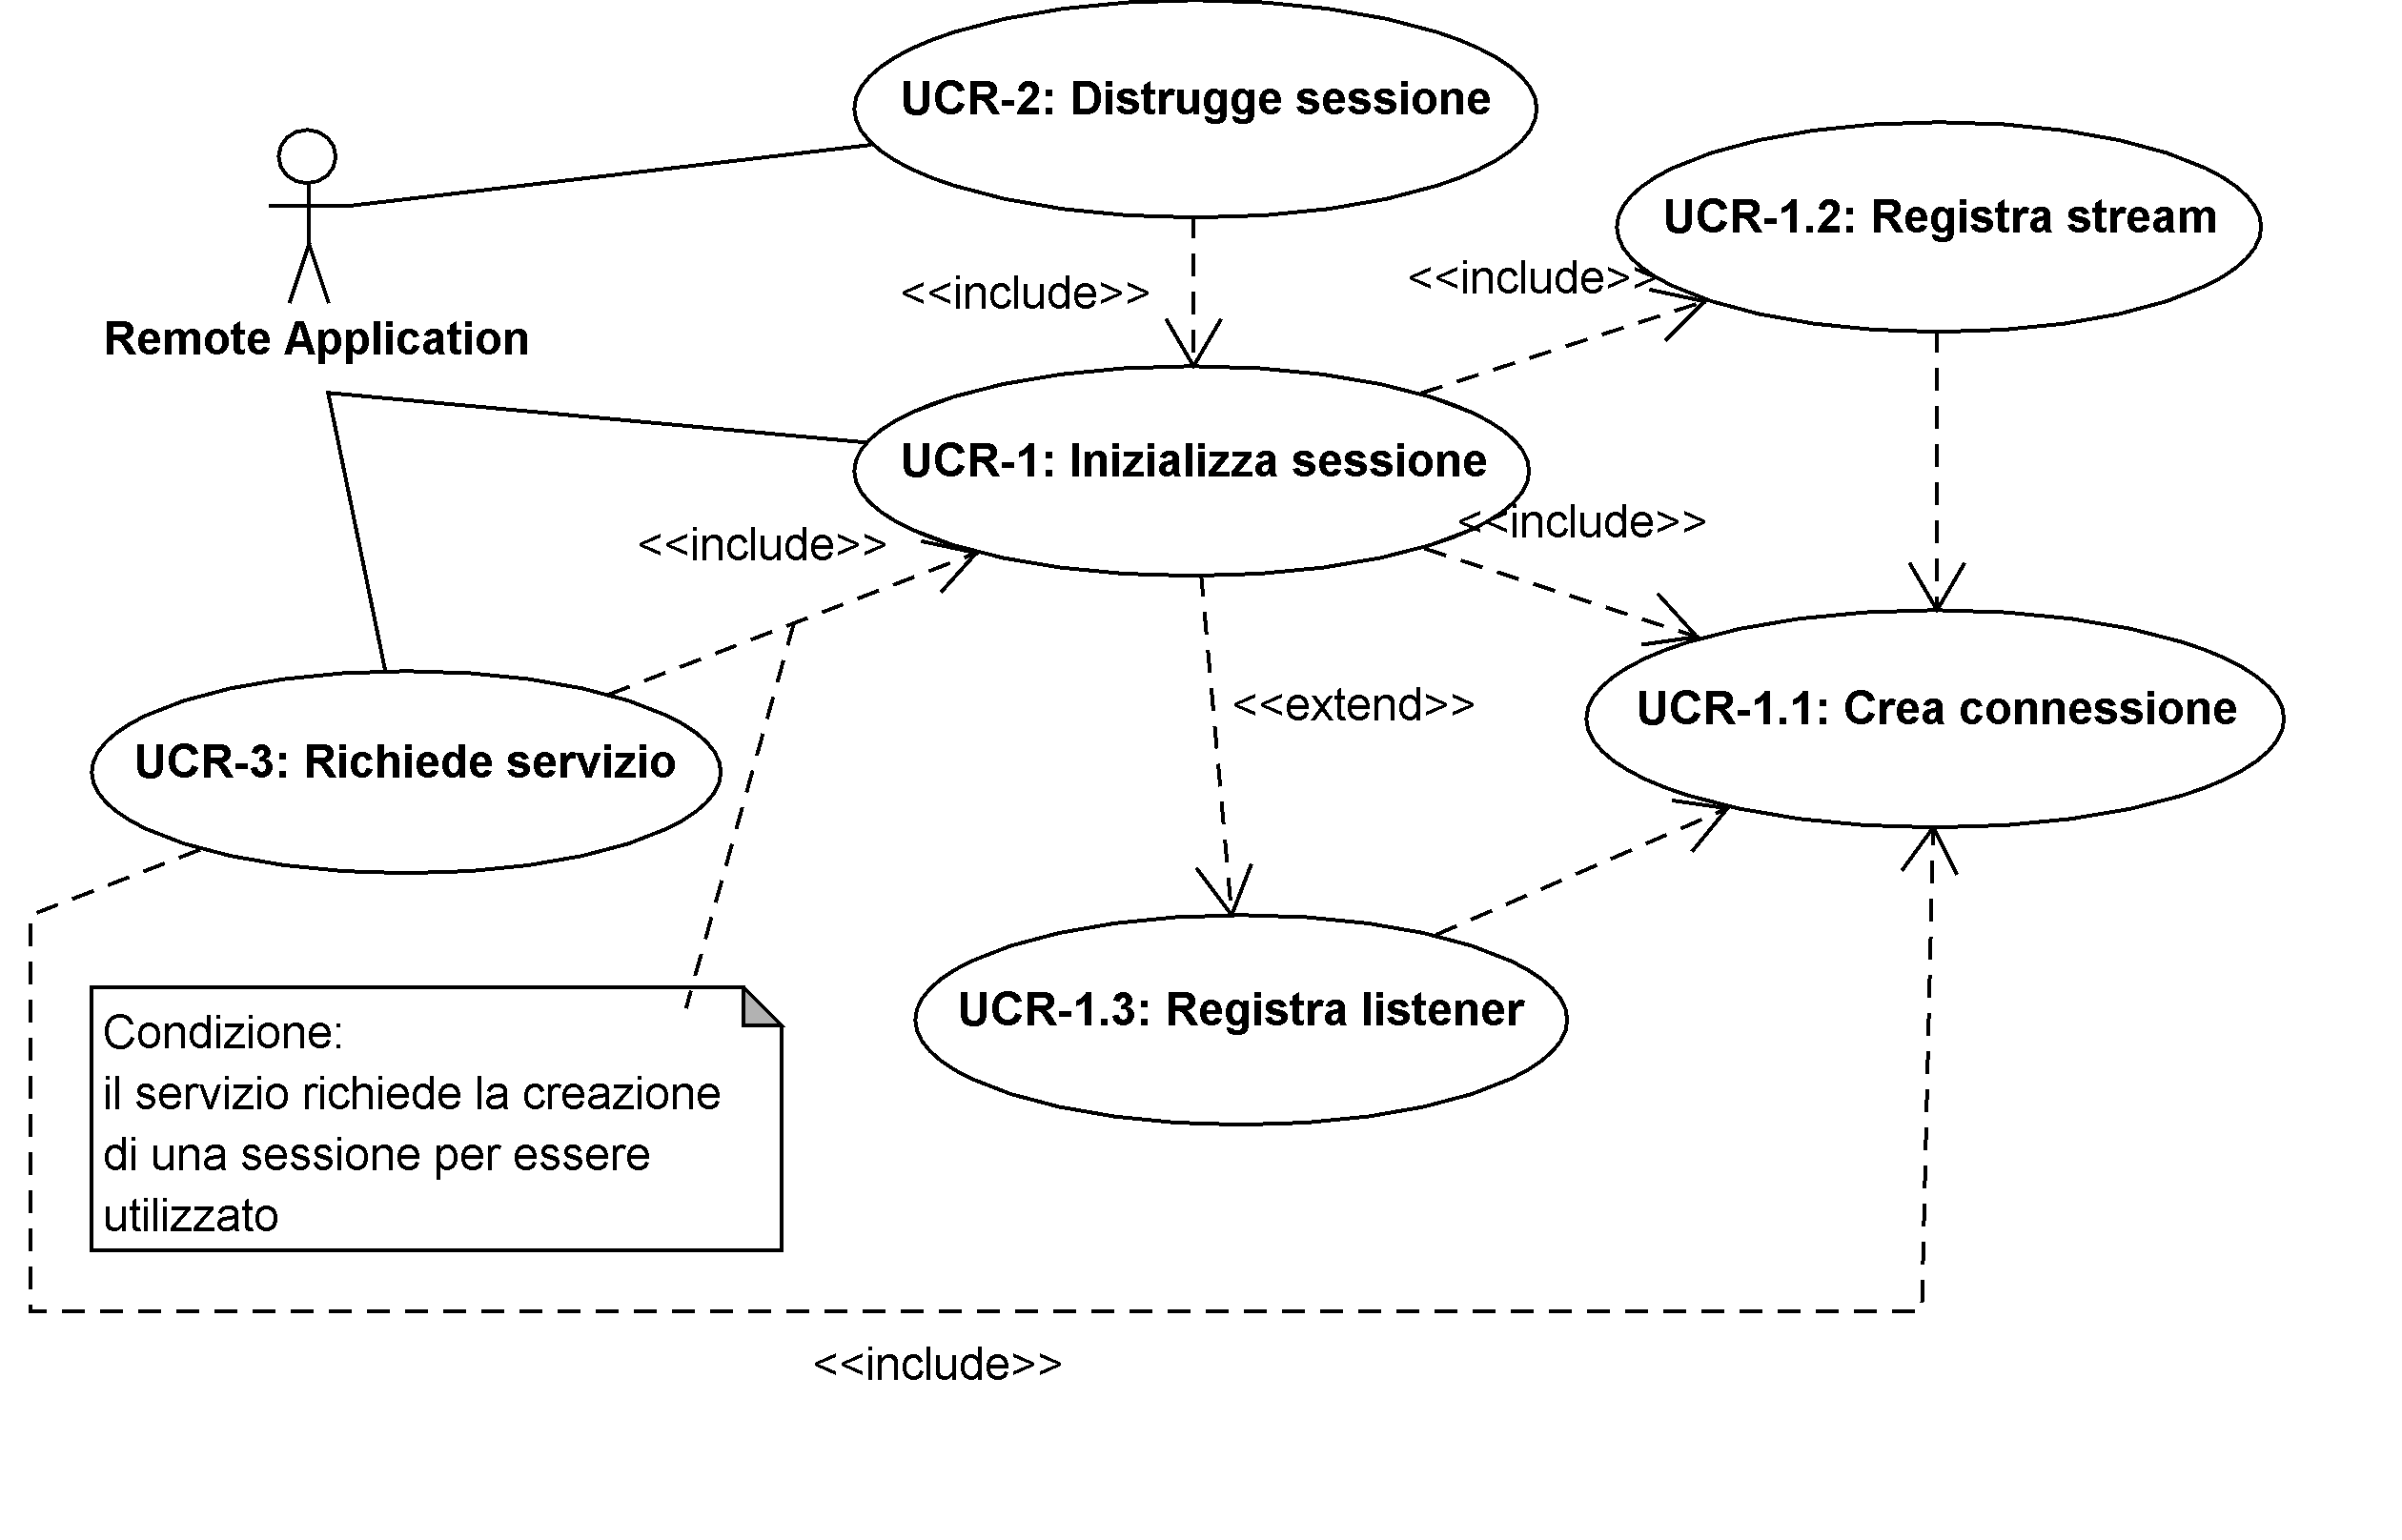
\includegraphics[width=1.1\textwidth]{Immagini/Capitolo2/UseCases/UCR-generale.png}
\caption{Diagramma dei casi d'uso UCR-1, UCR-2, UCR-3}\label{fig:uc-ucr-generale}
\end{figure}

Nel proseguo dei paragrafi relativi ai casi d'uso \emph{UCR}, il nome dell'attore \emph{Remote Application} verrà abbreviato con la sigla \emph{RA}.

\begin{itemize}
	\item \textbf{Attori:} Remote Application (\emph{RA})
	\item \textbf{Scopo e descrizione:} la RA deve avere la possibilità di inizializzare una sessione persistente con il software server che memorizzi le informazioni i dati che devono essere conservati fra richieste differenti
	\item \textbf{Pre-condizioni:} la RA ha conoscenza dei parametri di connessione relativi ad una istanza del software server
	\item \textbf{Post-condizioni:} la RA ottiene un codice univoco che identifica la sessione creata
	\item \textbf{Flusso principale degli eventi:}
		\begin{enumerate}
			\item la RA esegue una connessione con il server (si guardi il caso d'uso \emph{UCR-1.1})
			\item la RA richiede l'inizializzazione di una sessione
				\begin{itemize}
					\item la RA può fornire al server i parametri di connessione di uno stream (si guardi il caso d'uso \emph{UCR-1.2})
					\item la RA può fornire al server i parametri di connessione di un listener (si guardi il caso d'uso \emph{UCR-1.3})
				\end{itemize}
			\item la RA memorizza l'identificativo di sessione
		\end{enumerate}
	\item \textbf{Flusso alternativo:}
		\begin{enumerate}
			\setcounter{enumi}{1}
			\item se la RA non ottiene l'identificativo di sessione, lo scenario prosegue dal punto 1 del flusso principale
		\end{enumerate}
\end{itemize}


\paragraph{UCR-1.1: Crea connessione}

\begin{itemize}
	\item \textbf{Attori:} RA
	\item \textbf{Scopo e descrizione:} la RA deve avere la possibilità di stabilire una connessione con il server tramite protocollo XML-RPC
	\item \textbf{Pre-condizioni:} la RA ha conoscenza dei parametri di connessione relativi ad una istanza del software server
	\item \textbf{Post-condizioni:} la RA ha stabilito una connessione. Permette l'esecuzione dei casi d'uso \emph{UCR-1}, \emph{UCR-1.2}, \emph{UCR-1.3}, \emph{UCR-3}
	\item \textbf{Flusso principale degli eventi:}
		\begin{enumerate}
			\item la RA stabilisce una connessione seguendo le specifiche del protocollo XML-RPC
		\end{enumerate}
	\item \textbf{Flusso alternativo:}
		\begin{enumerate}
			\item se la connessione fallisce, la RA attiva un protocollo di gestione dell'errore (la definizione del protocollo è materia della RA)
		\end{enumerate}
\end{itemize}


\paragraph{UCR-1.2: Registra stream}

\begin{itemize}
	\item \textbf{Attori:} RA
	\item \textbf{Scopo e descrizione:} la RA deve essere in grado di registrare uno stream remoto utilizzabile dal software server 
	\item \textbf{Pre-condizioni:} la RA ha eseguito con successo il caso d'uso \emph{UCR-1.1}
	\item \textbf{Post-condizioni:} il software server può utilizzare lo stream remoto come sostituto di uno locale. Permette l'esecuzione dei casi d'uso \emph{UCC-1.2.1} e \emph{UCC-1.2.2} anche per l'attore RA
	\item \textbf{Flusso principale degli eventi:}
		\begin{enumerate}
			\item la RA fornisce al software server i parametri di connessione di uno stream remoto
			\item la RA indica:
				\begin{enumerate}
					\item indirizzo e porta di connessione dello stream
					\item nome dello stream remoto
					\item nome dello stream per il software server
					\item un codice di controllo
				\end{enumerate}
			\item la RA riceve un segnale di conferma all'indirizzo indicato usando i parametri forniti
			\item lo stream remoto è indicato come sostituto di uno stream locale
		\end{enumerate}
	\item \textbf{Flusso alternativo:}
		\begin{enumerate}
			\setcounter{enumi}{2}
			\item se la RA non ottiene un segnale di conferma dopo un tempo massimo stabilito, la RA attiva un protocollo di gestione dell'errore (la definizione del protocollo è materia della RA)
			\item lo stream remoto viene ignorato
		\end{enumerate}
\end{itemize}


\paragraph{UCR-1.3: Registra listener}

\begin{itemize}
	\item \textbf{Attori:} RA
	\item \textbf{Scopo e descrizione:} la RA deve essere in grado di registrare un listener remoto utilizzabile dal software server 
	\item \textbf{Pre-condizioni:} la RA ha eseguito con successo il caso d'uso \emph{UCR-1.1}
	\item \textbf{Post-condizioni:} il software server può utilizzare il listener remoto come sostituto di uno locale. Permette l'esecuzione del caso d'uso \emph{UCC-1.2.3} anche per l'attore RA
	\item \textbf{Flusso principale degli eventi:}
		\begin{enumerate}
			\item la RA fornisce al software server i parametri di connessione di un listener remoto
			\item la RA indica:
				\begin{enumerate}
					\item indirizzo e porta di connessione del listener
					\item nome del listener remoto
					\item nome del listener per il software server
					\item il nome degli eventi per i quali registrare il listener
					\item un codice di controllo
				\end{enumerate}
			\item la RA riceve un segnale di conferma all'indirizzo indicato usando i parametri forniti
			\item il listener remoto è indicato come sostituto di uno locale
		\end{enumerate}
	\item \textbf{Flusso alternativo:}
		\begin{enumerate}
			\setcounter{enumi}{2}
			\item se la RA non ottiene un segnale di conferma dopo un tempo massimo stabilito, la RA attiva un protocollo di gestione dell'errore (la definizione del protocollo è materia della RA)
			\item il listener remoto viene ignorato
		\end{enumerate}
\end{itemize}



\pagebreak

\subsubsection{UCR-2: Distrugge sessione}

%%UCR-2: Distrugge sessione

Il diagramma relativo al caso d'uso \emph{UCR-2}, data la natura complessa dello stesso, è accorpato a quello del caso d'uso \emph{UCR-1} fornito in \figurename~\ref{fig:uc-ucr-generale}.

\begin{itemize}
	\item \textbf{Attori:} RA
	\item \textbf{Scopo e descrizione:} la RA deve avere la possibilità di terminare e distruggere una sessione precedentemente inizializzata
	\item \textbf{Pre-condizioni:} la RA ha eseguito il caso d'uso \emph{UCR-1}
	\item \textbf{Post-condizioni:} il codice univoco ottenuto dall'esecuzione del caso d'uso \emph{UCR-1} non è più valido
	\item \textbf{Flusso principale degli eventi:}
		\begin{enumerate}
			\item la RA notifica la volontà di terminare la sessione al software server
			\item la RA riceve notifica di avvenuta chiusura della sessione
			\item la RA cancella dalla propria memoria il codice univoco di sessione
		\end{enumerate}
	\item \textbf{Flusso alternativo:}
		\begin{enumerate}
			\setcounter{enumi}{1}
			\item se la RA non riceve notifica di avvenuta chiusura della sessione dopo un tempo stabilito, notifica un avviso non invasivo
			\item lo scenario prosegue dal punto 3 del flusso principale
		\end{enumerate}
\end{itemize}
\pagebreak

\subsubsection{UCR-3: Richiede servizio}

%%UCR-3: Richiede servizio

Il diagramma relativo al caso d'uso \emph{UCR-3}, data la natura complessa dello stesso, è accorpato a quello del caso d'uso \emph{UCR-1} fornito in \figurename~\ref{fig:uc-ucr-generale}.

\begin{itemize}
	\item \textbf{Attori:} RA
	\item \textbf{Scopo e descrizione:} la RA deve avere la possibilità di richiedere un servizio al software server
	\item \textbf{Pre-condizioni:} la RA ha eseguito il caso d'uso \emph{UCR-1.1}. La RA ha eseguito il caso d'uso \emph{UCR-1} se il servizio richiesto richiede l'inizializzazione di una sessione
	\item \textbf{Post-condizioni:} la RA ha ottenuto il risultato dell'elaborazione effettuata da un servizio
	\item \textbf{Flusso principale degli eventi:}
		\begin{enumerate}
			\item la RA richiede un servizio al software server
				\begin{itemize}
					\item la RA indica il nome del servizio richiesto
					\item la RA indica i parametri di esecuzione del servizio
					\item la RA può indicare il codice univoco di una sessione precedentemente inizializzata, se necessario
				\end{itemize}
			\item la RA attende il completamento dell'elaborazione
		\end{enumerate}
	\item \textbf{Flusso alternativo \#1:}
		\begin{enumerate}
			\item se la RA richiede un servizio non disponibile, la RA riceve un messaggio d'errore
			\item la RA attiva un protocollo di gestione dell'errore (la definizione del protocollo è materia della RA)
		\end{enumerate}

	\item \textbf{Flusso alternativo \#2:}
		\begin{enumerate}
			\item se la RA richiede un servizio disponibile, ma il codice di sessione è scaduto
			\item la RA esegue il caso d'uso \emph{UCR-1}
			\item lo scenario prosegue dal punto 1 del flusso principale
		\end{enumerate}

		
	\item \textbf{Flusso alternativo \#3:}
		\begin{enumerate}
			\setcounter{enumi}{1}
			\item se la RA non riceve risposta entro un tempo limite, la RA attiva un protocollo di gestione dell'errore (la definizione del protocollo è materia della RA)
		\end{enumerate}
\end{itemize}
\pagebreak


\section{Requisiti}

\subsection{Generale}


\chapter{Progettazione}



\chapter*{Conclusioni}
\addcontentsline{toc}{chapter}{Conclusioni e sviluppi futuri}
\chaptermark{Conclusioni}
\rhead{}

%\section{Conclusioni}


L'integrazione degli strumenti di sviluppo per sistemi esperti con tecnologie orientate alla distribuzione degli stessi in ambito \emph{web} ha offerto lo spunto per questo lavoro di tesi. Prendendo come riferimento le funzionalità offerte da un \emph{environment} di grande adozione come CLIPS, è stata progettata e quindi realizzata una soluzione compatibile che enfatizzasse le capacità di estensibilità e integrazione offerte dal linguaggio di programmazione scelto per la realizzazione del prototipo: Python. Al fine di saggiare la flessibilità della soluzione proposta è stata eseguita l'integrazione della soluzione in un modello d'architettura \emph{client-server} e quindi valutato l'impatto che l'adozione di questa tecnologia ha avuto sulle prestazioni complessive del sistema.

Durante questa trattazione è stata fornita una definizione di sistemi esperti, approfondendo le tematiche relative al loro processo di sviluppo e all'ambito di utilizzo degli stessi. L'attenzione è stata quindi focalizzata verso le tecniche utilizzate per la formalizzazione della conoscenza in strutture adeguate alla computazione e quindi offerta una classificazione generale degli strumenti di sviluppo per sistemi esperti.
Nella seconda e terza parte sono state approfondite le problematiche relative alla progettazione e alla realizzazione di un prototipo funzionante di \emph{environment} multi-paradigmatico, successivamente sottoposto ad una valutazione per testarne la correttezza e le prestazioni.

Da quanto osservato durante la sperimentazione si può affermare che i risultati ottenuti sono in linea con le attese. Il livello di compatibilità con il sistema di riferimento risulta soddisfacente, i costrutti più utilizzati e considerati indispensabili vengono resi disponibili dal prototipo e i comportamenti riscontrati risultano trovano corrispondenza fra i due sistemi. L'analisi della prestazione ha mostrato un \emph{gap} abbastanza evidente, ma il degrado delle prestazioni, superato un valore di soglia, replica esattamente il comportamento riscontrato nella soluzione di riferimento. Una delle cause alla base delle minori prestazioni è il linguaggio utilizzato per l'implementazione del prototipo, ma non è l'unica. L'analisi del grafico delle chiamate (\figurename~\ref{fig:profile-sudoku}) generato durante la profilazione del benchmark \emph{Sudoku} ha messo in luce due criticità, sicuramente concause delle scarse prestazioni ottenute nello specifico test:
\begin{enumerate}
	\item la realizzazione scelta per la rappresentazione dei Token nel sistema utilizza una struttura ad albero per ridurre il consumo di memoria e permettere una condivisione delle informazioni~\cite{Doorenbos95productionmatching}. Questo approccio ha comportato un maggior dispendio di tempo per l'esecuzione delle procedure di \emph{matching} a causa della forma utilizzata per serializzazione delle regole nello specifico test.
	
	\item l'implementazione dei pattern \emph{Test-CE} prevede l'esecuzione di chiamate a funzione senza prevedere alcun sistema di \emph{caching} dei risultati. Verifiche successive richiedono una nuova esecuzione della funzione anche nei casi in cui gli input siano identici a quelli di valutazioni precedenti.
\end{enumerate}



%Il risultato di questo lavoro è un sistema che può rappresentare una buona base di partenza per ulteriori evoluzioni del sistema. 
%Le capacità realizzate rappresentano una porzione delle funzionalità che vengono richieste ad un \emph{environment per sistemi esperti} della corrente generazione. Le scelte effettuate durante la progettazione e la realizzazione del sistema hanno avuto come priorità quella di rendere il sistema modificabile, analizzabile ed estendibile con facilità. Lo sviluppo della componente server è stato un modo per saggiarne la flessibilità trasferendo il normale modello di interazione anche attraverso un'architettura tanto differente quanto quella \emph{client-server}.


\section*{Sviluppi futuri}

L'approfondimento di alcune delle mancanze del prototipo o l'aggiunta di ulteriori funzionalità potrebbe offrire lo spunto per ulteriori evoluzioni del sistema e nuovi ambiti di ricerca:
\begin{itemize}
	\item l'integrazione di un \emph{regime di controllo} alternativo basato sul \emph{backward-chaining} o su approcci ibridi, garantendo agli ingegneri della conoscenza maggiore flessibilità durante le fasi di progettazione.
	
	\item l'integrazione del paradigma di programmazione basato su oggetti nel linguaggio di specifica.
	
	\item la valutazione delle prestazioni offerte dal sistema utilizzando algoritmi di matching differenti come ad esempio TREAT~\cite{Miranker:1987:TBM:899610}~\cite{Miranker:1987:TBM:1856670.1856678} o LEAPS~\cite{Batory:1994:LA:899216}.	
	
	\item approfondimento delle problematiche relative alle prestazioni generali del sistema, eseguendo una nuova valutazione sulle tecnologie impiegate per la realizzazione dell'artefatto.
	
	\item l'integrazione di funzionalità che agevolino lo svolgimento di attività comuni  dei sistemi esperti come la spiegazione dell'inferenza.
	
	\item la fusione nel motore inferenziale di strumenti per la gestione dell'incertezza e della logica \emph{Fuzzy}.
\end{itemize}

\pagebreak
\lhead{\emph{BIBLIOGRAFIA}}
\rhead{}
\appendix
\addcontentsline{toc}{chapter}{\bibname}
\onehalfspacing
\printbibliography
\setcounter{chapter}{1}
\setcounter{program}{0}

\chapter*{Appendici}
\addcontentsline{toc}{chapter}{Appendici}
\section*{Artefatti per la valutazione del sistema}
\addcontentsline{toc}{section}{Artefatti per la valutazione del sistema}
\subsection*{Problema dell'agricoltore, variante 1}
\begin{program}
\verbatimtabinput[2]{Artefatti/Agricoltore-1-a.txt}
%\lstinputlisting[breaklines]{Artefatti/Agricoltore-1.txt}
\caption{Problema dell'agricoltore: formulazione 1}\label{code:agricoltore-1}
\end{program}
\begin{program}
\verbatimtabinput[2]{Artefatti/Agricoltore-1-b.txt}
\end{program}
\begin{program}
\verbatimtabinput[2]{Artefatti/Agricoltore-1-c.txt}
\end{program}
\begin{program}
\verbatimtabinput[2]{Artefatti/Agricoltore-1-d.txt}
\end{program}
\begin{program}
\verbatimtabinput[2]{Artefatti/Agricoltore-1-e.txt}
\end{program}

\subsection*{Problema dell'agricoltore, variante 2}
\begin{program}
\verbatimtabinput{Artefatti/Agricoltore-2.txt}
%\lstinputlisting[breaklines]{Artefatti/Agricoltore-2.txt}
\caption{Problema dell'agricoltore: formulazione 2}\label{code:agricoltore-2}
\end{program}
\subsection*{Sistema per la diagnosi}
\begin{program}
\verbatimtabinput{Artefatti/Diagnosi.txt}
%\lstinputlisting[breaklines]{Artefatti/Diagnosi.txt}
\caption{Sistema per la diagnosi}\label{code:diagnosi}
\end{program}

\pagebreak

\addcontentsline{toc}{section}{Specifica BNF della linguaggio accettato}
\section*{Specifica BNF del linguaggio accettato}

\begin{program}
\verbatimtabinput{Artefatti/BNF-linguaggio.txt}
\caption{Specifica BNF del linguaggio accettato}\label{code:bnf}
\end{program}


\end{document}
